%% Преамбула TeX-файла

% 1. Стиль и язык
\documentclass[utf8x, 12pt]{G7-32} % Стиль (по умолчанию будет 14pt)

\usepackage{gensymb}
\usepackage{multirow}
\usepackage{makecell}

% Остальные стандартные настройки убраны в preamble.inc.tex.
\sloppy

% Настройки стиля ГОСТ 7-32
% Для начала определяем, хотим мы или нет, чтобы рисунки и таблицы нумеровались в пределах раздела, или нам нужна сквозная нумерация.
\EqInChapter % формулы будут нумероваться в пределах раздела
\TableInChapter % таблицы будут нумероваться в пределах раздела
\PicInChapter % рисунки будут нумероваться в пределах раздела

% Добавляем гипертекстовое оглавление в PDF
\usepackage[
bookmarks=true, colorlinks=true, unicode=true,
urlcolor=black,linkcolor=black, anchorcolor=black,
citecolor=black, menucolor=black, filecolor=black,
]{hyperref}

% Изменение начертания шрифта --- после чего выглядит таймсоподобно.
% apt-get install scalable-cyrfonts-tex

\IfFileExists{cyrtimes.sty}
    {
        %\usepackage{cyrtimespatched}
    }
    {
        % А если Times нету, то будет CM...
    }

\usepackage{graphicx}   % Пакет для включения рисунков

% С такими оно полями оно работает по-умолчанию:
% \RequirePackage[left=20mm,right=10mm,top=20mm,bottom=20mm,headsep=0pt]{geometry}
% Если вас тошнит от поля в 10мм --- увеличивайте до 20-ти, ну и про переплёт не забывайте:
\geometry{right=20mm}
\geometry{left=30mm}


% Пакет Tikz
\usepackage{tikz}
\usetikzlibrary{arrows,positioning,shadows}

% Произвольная нумерация списков.
\usepackage{enumerate}


% Настройки листингов.
% 8 Листинги

\usepackage{listings}

% Значения по умолчанию
\lstset{
  basicstyle= \footnotesize,
  breakatwhitespace=true,% разрыв строк только на whitespacce
  breaklines=true,       % переносить длинные строки
%   captionpos=b,          % подписи снизу -- вроде не надо
  inputencoding=koi8-r,
  numbers=left,          % нумерация слева
  numberstyle=\footnotesize,
  showspaces=false,      % показывать пробелы подчеркиваниями -- идиотизм 70-х годов
  showstringspaces=false,
  showtabs=false,        % и табы тоже
  stepnumber=1,
  tabsize=4,              % кому нужны табы по 8 символов?
  frame=single
}

% Стиль для псевдокода: строчки обычно короткие, поэтому размер шрифта побольше
\lstdefinestyle{pseudocode}{
  basicstyle=\small,
  keywordstyle=\color{black}\bfseries\underbar,
  language=Pseudocode,
  numberstyle=\footnotesize,
  commentstyle=\footnotesize\it
}

% Стиль для обычного кода: маленький шрифт
\lstdefinestyle{realcode}{
  basicstyle=\scriptsize,
  numberstyle=\footnotesize
}

% Стиль для коротких кусков обычного кода: средний шрифт
\lstdefinestyle{simplecode}{
  basicstyle=\footnotesize,
  numberstyle=\footnotesize
}

% Стиль для BNF
\lstdefinestyle{grammar}{
  basicstyle=\footnotesize,
  numberstyle=\footnotesize,
  stringstyle=\bfseries\ttfamily,
  language=BNF
}

% Определим свой язык для написания псевдокодов на основе Python
\lstdefinelanguage[]{Pseudocode}[]{Python}{
  morekeywords={each,empty,wait,do},% ключевые слова добавлять сюда
  morecomment=[s]{\{}{\}},% комменты {а-ля Pascal} смотрятся нагляднее
  literate=% а сюда добавлять операторы, которые хотите отображать как мат. символы
    {->}{\ensuremath{$\rightarrow$}~}2%
    {<-}{\ensuremath{$\leftarrow$}~}2%
    {:=}{\ensuremath{$\leftarrow$}~}2%
    {<--}{\ensuremath{$\Longleftarrow$}~}2%
}[keywords,comments]

% Свой язык для задания грамматик в BNF
\lstdefinelanguage[]{BNF}[]{}{
  morekeywords={},
  morecomment=[s]{@}{@},
  morestring=[b]",%
  literate=%
    {->}{\ensuremath{$\rightarrow$}~}2%
    {*}{\ensuremath{$^*$}~}2%
    {+}{\ensuremath{$^+$}~}2%
    {|}{\ensuremath{$|$}~}2%
}[keywords,comments,strings]

% Подписи к листингам на русском языке.
\renewcommand\lstlistingname{\cyr\CYRL\cyri\cyrs\cyrt\cyri\cyrn\cyrg}
\renewcommand\lstlistlistingname{\cyr\CYRL\cyri\cyrs\cyrt\cyri\cyrn\cyrg\cyri}


% Полезные макросы листингов.
% Любимые команды
\newcommand{\Code}[1]{\textbf{#1}}


\begin{document}

\frontmatter % выключает нумерацию ВСЕГО; здесь начинаются ненумерованные главы: реферат, введение, глоссарий, сокращения и прочее.

% Команды \breakingbeforechapters и \nonbreakingbeforechapters
% управляют разрывом страницы перед главами.
% По-умолчанию страница разрывается.

% \nobreakingbeforechapters
% \breakingbeforechapters

% Также можно использовать \Referat, как в оригинале
\begin{abstract}

В данной дипломной работе рассмотрены вопросы разработки учебной
операционной системы.

В аналитическом разделе рассмотреты основы теории операционных систем. Рассмотрены
существующие операционные учебные системы. Рассмотрены сущесвтующие форматы исполняемых
файлов и средства виртуализации.

В конструкторском разделе описаны режимы работы процессора,
механизмы работы сегментного преобразования, страничного преобразования,
обработки прерываний, процесс перехода в длинный режим.

В технологическом разделе рассмотрены средства разработки и отладки, загрузка ОС,
организация памяти ОС. Описана реализация системных вызовов, многозадачности и
потоков ядра.

В организационно-экономическом разделе выполнено определение этапов работ.
Проведен рассчет трудоемкости выполняемых работ, определно количество исполнителей.
Проведены рассчеты по определению структуры затрат на разработку проекта, а также
произведено планирование цены ПО и прогнозирование прибыли.

В разделе охраны труда и экологии рассмотрены вредные факторы, влияющие на
пользователей при использовании ПО. Приведен рассчет воздухообмена в
компьютерном классе. Рассмотрен процесс утилизации пластмасс,
являющихся частью жидко-кристаллического монитора.

В заключении делаются выводы о результатах, достигнутых в ходе выполнения
данной работы.

\end{abstract}


\tableofcontents

\Defines
\begin{description}
\item[Байт] 8 бит.
\item[Слово] 2 байта.
\item[Двойное слово] 4 байта.
\item[16-битный режим] унаследованный режим или режим совместимости, в котором размер адреса по умолчанию составляет 16~бит.
\item[32-битный режим] унаследованный режим или режим совместимости, в котором размер адреса по умолчанию составляет 32~бита.
\item[64-битный режим] подрежим длинного режима. В данном режиме размер адреса по умолчанию составляет 64~бита и доступны
новые возможности, такие как расширенный набор регистров.
\item[Режим совместимости] подрежим длинного режима. В данном режиме размер адреса по умолчанию составляет 32 бита, он
позволяет запускать существующее 16 и 32-битное прикладное ПО без перекомпиляции.
\item[Унаследованный режим] режим работы процессора в котором существующее 16 и 32-битное ПО можно запустить без модификаций.
Включает 3 подрежима: реальный режим, защищенный режим, режим виртуального 8086.
\item[Длинный режим] режим работы процессора уникальный для архитектуры AMD64. Имеет 2 подрежима: 64-битный режим и
режим совместимости.
\item[Системное ПО] привилегированное ПО, которое управляет аппаратными ресурсами системы и контролирует доступ к этим ресурсам.
\item[Логический адрес] адрес до сегментного преобразования, включающий в себя сегментный регистр (селектор) и смещение.
\item[Эффективный адрес] смещение в сегменте.
\item[Линейный (виртуальный) адрес] адрес полученный в результате сегментного преобразования.
\item[Физический адрес] адрес в физическом адресном пространстве.
\item[Каноническая форма адреса] форма адреса, в которой все биты начиная с наиболее значимого (в данной реализации) и до 63го совпадают.
\item[Процесс] исполняющаяся программа, имеющая своё собственное
	виртуальное адресное пространство и свой контекст выполнения, включающий значения регистров ЦП.
\end{description}

\Abbreviations
\begin{description}
\item[ПО] программное обеспечение.
\item[SMM] System Management Mode, режим работы процессора, используемый, как правило
для настройки аппаратного обеспечения.
\item[SMI] System Management Interrupt, прерывание, при возникновении которого, процессор
переходит в SMM.
\item[CPL] текущий уровень привилегий процессора.
\item[DPL] уровень привилегий дескриптора.
\item[GDT] глобальная таблица дескрипторов.
\item[IDT] таблица дескрипторов прерываний.
\item[IST] таблица указателей стека в длинном режиме.
\item[LDT] локальная таблица дескрипторов.
\item[TSS] сегмент состояния задачи.
\item[PAE] механизм расширения физических адресов, позволяет использовать физические адреса длинной
до 52 бит.
\item[EFER] моделезависимый регистр включения расширенных возможностей.
\item[FLAGS] 16-битный регистр флагов.
\item[eFLAGS] 16 или 32-битный регистр флагов.
\item[EFLAGS] 32-битный регистр флагов.
\item[rFLAGS] 16, 32 или 64-битный регистр флагов.
\item[RFLAGS] 64-битный регистр флагов.
\item[IP] 16-битный счетчик команд.
\item[eIP] 16 или 32-битный счетчик команд.
\item[EIP] 32-битный счетчик команд.
\item[rIP] 16, 32 или 64-битный счетчик команд.
\item[RIP] 64-битный счетчик команд.
\item[CS] регистр сегмента кода.
\item[CR0,CR2-CR4,CR8] управляющие регистры процессора.
\item[MSR] моделезависимый регистр.
\item[CPU] % FIXME
\item[APIC] % FIXME
\item[IOAPIC] % FIXME
\end{description}




\Introduction

Для изучения основ функционирования операционных систем недостаточно
изучения одного теоретического материала: для понимания работы ядра
ОС нужно изучить и его исходные коды.

Хотя в настоящее время ядра многих эксплуатируемых ОС доступны для
такого изучения, все они как возможный методический материал для
учебного процесса обладают двумя недостатками: высокой сложностью
и большим объемом исходных текстов. По этой причине коллективом
сотрудников университета MIT была разработана учебная операционная
система, позже названная JOS, предназначенная для практической
части курса разработки операционных систем.

Помимо своей компактности, JOS как учебная система обладает ещё одним
достоинством: студент работает со все более усложняющимися вариантами
системы, постепенно знакомясь с теми или иными функциями ядра ОС.
Исходные тексты JOS имеют лицензию MIT или BSD, т.е. она является
свободным программным обеспечением и может использоваться с минимальными
ограничениями.

Однако JOS имеет один существенный недостаток: она разработана для
устаревшей архитектуры x86.

Таким образом разработка учебной операционной системы для более современной
архитекруты AMD64 является актуальной задачей.


\mainmatter % это включает нумерацию глав и секций в документе ниже

\chapter{Аналитический раздел}
\label{cha:analysis}

\section{История процессоров x86}
Первым процессором из линейки x86 был процессор Intel 8086 -- 16-разрядный процессор с адресным пространством
равным 1~Мб. За ним последовали 80186 и 80286 (i286), в последнем появился защищенный режим, в котором можно
было адресовать до 1~Гб памяти. Следующим был процессор 80386 (i386), который позволял адресовать 4~Гб физической
памяти и имел страничное преобразование (для реализации виртуального адресного пространства). Последующие
поколения добавляли новые возможности: встроенный сопроцессор, кэш-память, PAE, MMX, SSE, SSE2 и т.д.

В начале 2000-х годов стало очевидно, что 32-битного адресного пространства недостаточно для приложений,
работающих с большими объемами данных (например с видео и базами данных), т.к. в этом случае процессор
может использовать только 4~гигабайта виртуального адресного пространства.

Для решения этой проблемы компания Intel разработала спецификацию IA-64 (исользуется в процессорах семейства
Itanium). Для сохранения обработной совместимости с унаследованным 32-битным ПО, в данной архитектуре использовался
режим эмуляции, который уступал по производительности оригинальным процессорам x86.

Компания AMD предложила другое решение: она добавила 64-битное расширение к существующей 32-разрядной архитектуре x86.
Это позволило использовать физические адреса длинной до 52~бит (архитектурный предел). Данная архитектура была
названа x86-64, а затем переименована в AMD64.

Успех процессоров на базе AMD64 привел к тому, что Intel лицензировала набор инструкций AMD64. Новая версия архитектуры
получила название EM64T (IA-32e), позже была переименована в Intel 64.


\section{Режимы работы процессора}
Унаследованная (legacy) архитектура x86 предусматривает четыре режима работы процессора:
\begin{enumerate}[1.]
	\item Реальный режим (англ. Real Mode)
	\item Защищенный режим (англ. Protected Mode)
	\item Режим виртуального 8086 (англ. Virtual-8086 Mode)
	\item Режим системного управления (англ. System Management Mode)
\end{enumerate}

Архитектура AMD64 поддерживает все эти режимы и добавляет новый режим,
названный <<длинный>> режим (англ. Long Mode).


\subsection{Унаследованный режим}
Унаследованный режим состоит из трех подрежимов: реальный режим, защищенный режим и режим виртуального 8086.
Страничное преобразование в защищенном режиме не является обязательным. Унаследованный режим сохраняет
бинарную совместимость не только с существующим 16-битным и 32-битным прикладным ПО, но и с существующим
16-битным и 32-битным системым ПО.

\paragraph{Реальный режим.}
В данном режиме, также называемом режимом реальных адресов, процессору доступен 1~мегабайт физической памяти.
Обработка прерываний и формирование адреса выполняется так же, как и реальном режиме процессора 80286.
Страничное преобразование адреса не поддерживается. Все ПО выполняется на нулевом уровне привилегий.

Процессор начинает работу в реальном режиме.

\paragraph{Защищенный режим.}
В данном режиме процессору доступно 4~гигабайта физической и виртуальной памяти. Доступны все возможности
сегментного преобразования и аппаратного переключения задач. Если страничное преобразование не используется --
виртуальные адреса совпадают с физическими.

В защищенном режиме ПО выполняется на уровнях привилегий 0-3. Как правило, прикладное ПО выполняется на третьем
уровне привилегий, а системное - на 0, 1 и 2.


\subsection{Длинный режим}
Длинный режим включает в себя 2 подрежима: 64-битный режим и режим совместимости.
64-битный режим поддерживает несколько новых возможностей, включая возможность
использовать 64-битное адресное пространство. Режим совместимости обеспечивает
бинарную совместимость с существующим 16-битным и 32-битным прикладным ПО при работе
в 64-битном окружении.

Перед активацией и переходом в длинный режим, операционная система должна перейти в
защищенный режим. Процесс перехода в длинный режим описан в главе~\ref{sec:long_mode_activation}.

\subsection{64-битный режим}
64-битный режим -- подрежим длинного режима, предусматривает поддержку 64-разрядного
ПО. Режим имеет следующие особенности:
\begin{enumerate}[1.]
\item 64-битные виртуальные адреса.
\item Доступ к битам 63:32 регистров общего назначения.
\item Дополнительные 8 регистров общего назначения (R8-R15).
\item 64-битный счетчик команд (RIP).
\item Плоская модель памяти с одним сегментом кода, данных и стека.
\end{enumerate}

Данный режим может быть активирован системным ПО для различных сегментов кода. В данном режиме
механизм сегментного преобразования адреса отключен. Для управления памятью используется
механизм страничного преобразования.

Следует обратить внимание на то, что В 64-битном режиме процессор может использовать
52-битные физические адреса (архитектурный предел) и 64-битные виртуальные адреса (из них
только первые 48 бит используются механизмом страничного преобразования).

\subsection{Режим совместимости}
Режим совместимости -- подрежим длинного режима, позволяет системному ПО обеспечивать
бинарную совместимость с существущим 16-битным и 32-битным прикладным ПО,
т.е. запускать данное ПО без перекомпиляции в 64-битной ОС в длинном режим.

В режиме совместимости, приложениям доступны только первые 4 гигабайта виртуального адресного пространства.

В данном режиме сегментное преобразование адреса работает так же, как и в унаследованной
архитектуре x86. С точки зрения прикладного ПО, режим совместимости не отличается от унаследованного
защищенного режима. С точки зрения системного ПО -- необходимо использовать механизмы длинного режима для
преобразования адресов и обработки исключений и прерываний.

В данной работе режим совместимости будет использоваться только для перехода
в 64-битный режим.


\section{Системные ресурсы}
Операционная система выполняет системные операции (управление памятью, изменение режима работы процессора и др.)
используя системные ресурсы. Эти ресурсы состоят из системных регистров (управляющих и моделезависимых)
и системных структур данных (различные таблицы).

Для доступа к моделезависимым регистрам (англ. MSR) используются команды RDMSR и WRMSR.
Данные команды предполагают что в регистре ECX находится номер регистра. Команда RDMSR
сохраняет значение MSR в регистры EDX:EAX (все MSR имеют размер 64 бита). Команда WRMSR
записывает в регистр MSR значение, содержащееся в EDX:EAX.

\subsection*{Управляющие регистры}
Регистры, управляющие работой процессора в архитектуре AMD64, включают:
\begin{description}
	\item[CR0] Позволяет изменять ражим работы процессора и управляет некоторыми возможностями процессора.
	\item[CR2] Используется механизмом страничного преобразования. При возникновении страничного исключения, содержит
		виртуальный адрес по которому произошло исключение.
	\item[CR3] Используется механизмом страничного преобразования. Содержит базовый адрес таблицы страниц верхнего
		уровня, управляет кешированием данной таблицы.
	\item[CR4] Содержит дополнительные флаги для различных возможностей процессора.
	\item[CR8] Используется для управления приоритетами внешних прерываний.
	\item[RFLAGS] Хранит состояние процессора и некоторые управляющие флаги. В основном, используется для
		управления аппаратным переключением задач, прерываниями и режимом виртуального 8086.
	\item[EFER] моделезависимый регистр, содержащий состояние процессора и управляющие флаги, для
		возможностей, которые не управляются регистрами CR0 и CR4. Для доступа к данному MSR в регистр
		ECX нужно занести значение \textbf{0xC000\,0080}.
\end{description}

В унаследованном режиме все управляющие регистры, в т.ч. RFLAGS -- 32-битные. EFER -- 64-битный во всех режимах.
Архитектура AMD64 расширяет все 32-битные управляющие регистры до 64 бит.

Далее в работе под обозначением \textbf{rFLAGS} будет иметься в виду 16-битный, 32-битный или
64-битный регистр флагов. Аналогично, \textbf{rIP} -- 16-битный, 32-битный или 64-битный счетчик комманд.


\section{Сегментное преобразование адреса}
Унаследованная архитектура x86 поддерживает механизм сегментного преобразования адреса, который
позволяет системному ПО создавать отдельное виртуальное адресное пространство для каждого процесса.
Размер и расположение сегмента в виртуальном адресном пространстве произвольны. Инструкции и данные
могут располагаться как в одном, так и в нескольких сегментах, каждому из которых будут назначены
отдельные атрибуты доступа.

Механизм сегментного преобразования использует 10 сегментных регистров, каждый из которых
определяет один сегмент. 6 из этих регистров (CS, DS, ES, FS, GS и SS) определяют пользовательские сегменты.
Пользовательские сегменты содержат команды, данные и стек. Они доступны как для системного, так и для прикладного ПО.
Оставшиеся 4 регистра (GDTR, LDTR, IDTR и TR) определяют системные сегменты. Системные сегменты содержат структуры
данных инициализируемые и используемые только системным ПО. Сегментные регистры содержат (в теневой части)
базовый адрес, указывающий на начало сегмента, лимит сегмента и атрибуты доступа.

Несмотря на то, что сегментное преобразование обеспечивает высокую гибкость в изоляции и защите данных,
обычно, эти задачи решаются эффективнее с использованием программной и аппаратной
поддержки страничного преобразования. По этой причине большинство современных систем не используют
сегментное преобразование.

В длинном режиме, работа сегментного преобразования зависит от того, в каком из подрежимов находится процессор:
\begin{itemize}
\item В режиме совместимости сегментное преобразование работает так же, как и в унаследованном режиме.
\item В 64-битном режиме сегментное преобразование отключено, задавая плоское 64-битное адресное пространство.
	Однако некоторые функции сегментых регистров (в частности системных сегментных регистров) продолжают использоваться.
\end{itemize}

Системное ПО может использовать механизм сегментного преобразования для реализации одной из двух основных
моделей: плоская модель памяти (используется один сегмент) и мульти-сегментная модель памяти
(используется несколько сегментов).

\subsubsection*{Плоская модель памяти}
Плоская модель памяти -- это простейшая форма сегментного преобразования. Плоская модель памяти позволяет
системному ПО обойти часть механизмов сегментного преобразования. В плоской модели памяти все базовые адреса
сегментов равны 0, а лимиты сегментов равны 4 гигабайтам. Установка базового адреса сегмента в 0 фактически
отключает сегментное преобразование (сегмент:смещение = смещение).

\subsubsection*{Сегментное преобразование в 64-битном режиме}
В 64-битном режиме сегментное преобразование отключено. Аппаратное обеспечение игнорирует значение
базового адреса сегмента и обрабатывает его как 0. Игнорируются размер и большинство атрибутов.
Системные сегментные регистры всегда используются в 64-битном режиме.

\subsection{Структуры данных сегментного преобразования}
Механизм сегментного преобразования использует следующие структуры данных:
\begin{itemize}
\item Дескрипторы сегментов. Описывают сегменты (базовый адрес сегмента в виртуальном
	адресном пространстве, его лимит, атрибуты доступа и некоторые другие характеристики).
\item Таблицы дескрипторов. Сегментные дескрипторы хранятся в памяти в одной из трех таблиц: GDT, LDT, IDT.
\item Сегмент состояния задачи (TSS). Cпециальный тип системного сегмента, который содержит
	информацию о состоянии процесса (задачи), в т.ч. ссылки на необходимые процессу структуры данных.
\item Сегментные селекторы. Используются для выбора дескрипторов из таблиц дескрипторов.
\end{itemize}

Механизм сегментного преобразования использует следующие регистры: CS, DS, ES, SS, GS, FS, GDTR, IDTR, LDTR, TR.
Структуры данных связаны с регистрами следующим образом:
\begin{itemize}
	\item Сегментные регистры (CS, DS, ES, FS, GS, SS). Используются чтобы ссылаться
		на пользовательские сегменты. При загрузке селектора сегмента в сегментный регистр процессор
		автоматически загружает выбранный дескриптор в теневую часть сегментного регистра.
	\item Регистры таблиц дескрипторов (GDTR, LDTR, IDTR). Задают виртуальный базовый адрес и лимит таблиц дескрипторов.
	\item Регистр задачи (TR). Задает положение и размер текущего сегмента состояния задачи (TSS).
\end{itemize}

\subsubsection*{Сегментные селекторы}
Селекторы сегментов указывают на дескрипторы в GDT и LDT.
Формат селектора сегмента показан на рис.~\ref{fig:segment-selector}.

\begin{figure}[ht!]
  \centering
  \includegraphics[width=0.4\textwidth]{inc/dia/segment-selector}
  \caption{Формат селектора сегмента}
  \label{fig:segment-selector}
\end{figure}

Селектор состоит из следующих полей:
\begin{enumerate}[1.]
\item Индекс. Биты 15:3. Указывает на элемент в таблице дескрипторов.
	Дескрипторы имеют размер 8~байт, поэтому индекс умножается на 8
	чтобы получить смещение в таблице дескрипторов. Смещение прибавляется
	к базовому адресу GDT или LDT (в зависимости от значения TI), чтобы получить
	виртуальный адрес дескриптора.

	Некоторые элементы таблицы дескрипторов имееют размер 16~байт, вместо 8.
	Они занимают 2 элемента в таблице. Однако в длинном режиме смещение по
	прежнему вычисляется путем умножения индекса на 8. Системное ПО должно
	назначать селекторы так, чтобы они указывали на начало расширенных элементов.
\item Индикатор таблицы (TI). Бит 2. Указывает в какой таблице хранится дескриптор.
	Если бит сброшен в 0, это означает что селектор ссылается на запись в GDT.
	Иначе - селектор ссылается на запись в LDT.
\item Уровень привилегий (RPL). Биты 1:0. Равен уровню привилегий на котором
	находился процессор (CPL) при создании селектора. Используется для проверки прав доступа.
\end{enumerate}

Нулевые селекторы (индекс 0 и TI=0) используются чтобы сделать сегментные
регистры недействительными (аналог нулевых указателей).
При использовании сегментного регистра (не в 64-битном режиме),
содержащего нулевой селектор произойдет исключение \#GP.

\subsubsection*{Сегментные регистры}
Для улучшения производительности, при загрузке нового значения в сегментный регистр,
процессор загружает дескриптор, соответсвующий селектору, в теневую часть сегментного регистра.
Благодаря этому снижается число обращений к памяти.

На рис.~\ref{fig:segment-register-format-x86} показаны видимая и теневая части сегментного регистра.
ПО не имеет прямого доступа к теневой части сегментных регистров (кроме GS и FS).

\begin{figure}[ht!]
  \centering
  \includegraphics[width=0.4\textwidth]{inc/dia/segment-register-format-x86}
  \caption{Формат сегментного регистра}
  \label{fig:segment-register-format-x86}
\end{figure}

При вычислении адреса, базовый адрес считается равным 0, выход за пределы сегмента не проверяется.
Вместо этого выполняется проверка, что адрес находится в канонической форме. Содержимое теневой части
регистров DS, ES и SS игнорируется полностью.

\subsection{Таблицы дескрипторов}
Механизм сегментного преобразования использует таблицы дескрипторов.
Эти таблицы содержат дескрипторы, которые описывают расположение сегмента в виртуальной памяти,
его лимит (размер - 1) и атрибуты доступа. Обращение к полям дескриптора происходит при каждом
обращении к памяти (выборка инструкций, чтение/запись данных).

Как было сказано ранее, архитектура x86 поддерживает 3 типа таблиц дескрипторов: GDT, LDT (как правило, не используется), IDT.

\subsubsection*{GDT}
Для перехода в защищенный режим необходимо создать GDT. GDT содержит дескрипторы
сегментов кода и данных для сегментов, которые являются общими для всех задач.
Кроме пользовательских сегментов, GDT может содержать дескрипторы шлюзов и
другие системные дескрипторы. Системное ПО может расположить GDT в произвольной
области памяти, недоступной непривилегированному ПО.

На рис.~\ref{fig:gdt-ldt-access} показано как происходит доступ к GDT/LDT.

\begin{figure}[ht!]
  \centering
  \includegraphics[width=1.0\textwidth]{inc/dia/gdt-ldt-access}
  \caption{Доступ к GDT/LDT}
  \label{fig:gdt-ldt-access}
\end{figure}

\subsubsection*{Регистр глобальной таблицы дескрипторов}
Регистр GDT (GDTR) содержит базовый адрес и размер GDT. Регистр загружается командой LGDT.
На рис.~\ref{fig:gdtr-idtr-legacy-format} показан формат GDTR в унаследованном режиме и
режиме совместимости. На рис.~\ref{fig:gdtr-idtr-x64-format} показан формат GDTR в длинном режиме.

\begin{figure}[ht!]
  \centering
  \includegraphics[width=.4\textwidth]{inc/dia/gdtr-idtr-legacy-format}
  \caption{Формат GDTR и IDTR в унаследованном режиме}
  \label{fig:gdtr-idtr-legacy-format}
\end{figure}

\begin{figure}[ht!]
  \centering
  \includegraphics[width=.9\textwidth]{inc/dia/gdtr-idtr-x64-format}
  \caption{Формат GDTR и IDTR в длинном режиме}
  \label{fig:gdtr-idtr-x64-format}
\end{figure}

GDTR состоит из двух полей:
\begin{description}
\item[Лимит] 2 байта. Задает лимит GDT в байтах. При обращении ПО за пределы GDT произойдет
	исключение \#GP.
\item[Базовый адрес] 8 байт. Содержит виртуальный адрес начала таблицы. GDT может быть расположена
	по любому адресу, однако системному ПО следует использовать адрес, выровненный по 4-байтной границе,
	чтобы избежать снижения производительности из-за доступа к невыровненным данным.
\end{description}

В архитектуре AMD64 размер базового адреса в GDTR увеличен до 64 бит, что позволяет системному ПО,
работающему в длинном режиме, расположить GDT в произвольном месте 64-битного адресного пространства.
В унаследованном режиме процессор игнорирует старшие 4 байта.


\subsubsection*{IDT}
IDT, так же как GDT и LDT, может быть расположена в произвольной области памяти, недоступной непривилегированному ПО.

IDT может содержать дескрипторы следующих типов:
\begin{itemize}
	\item Шлюз прерывания (англ. interrupt gate)
	\item Шлюз ловушки (англ. trap gate)
	\item Шлюз задачи (англ. task gate)
\end{itemize}

В главе ~\ref{sec:exceptions_and_interrupts} описано,
как механизм обработки прерываний использует дескрипторы шлюзов.

Обращение к элементам IDT происходит по номеру вектора прерывания. Смещение в таблице вычисляется путем
умножения номера вектора прерывания на размер элемента таблицы. Размер элемента таблицы зависит от
режима работы процессора следующим образом:
\begin{itemize}
\item В длинном режиме размер элемента IDT составляет 16 байт.
\item В унаследованном режиме размер элемента IDT составляет 8 байт.
\end{itemize}

На рис.~\ref{fig:indexing-an-idt} показано, как происходит индексация в IDT по номерy вектора прерывания.

\begin{figure}[ht!]
  \centering
  \includegraphics[width=1.0\textwidth]{inc/dia/indexing-an-idt}
  \caption{Индексация в IDT}
  \label{fig:indexing-an-idt}
\end{figure}


\subsubsection*{Регистр IDT}
Регистр IDT (IDTR) содержит базовый адрес и размер IDT.
Содержимое регистра загружается командой LIDT. Формат IDTR совпадает с форматом GDTR во
всех режимах работы процессора. На рис.~\ref{fig:gdtr-idtr-legacy-format} показан формат
IDT в унаследованном режиме, а на рис.~\ref{fig:gdtr-idtr-x64-format} -- в длинном режиме.

\subsection{Унаследованные дескрипторы сегментов}
\subsubsection*{Формат дескриптора}
Дескрипторы сегментов определяют и изолируют сегменты друг от друга. Существует 2 основных типа
дескрипторов, каждый из которых используется для описания сегментов (шлюзов) разных типов:
\begin{itemize}
	\item Дескрипторы пользовательских сегментов -- дескрипторы сегментов кода и данных (в т.ч. стека).
	\item Дескрипторы системных сегментов -- дескрипторы LDT, TSS и шлюзов (описывают программные точки входа).
\end{itemize}

На рис.~\ref{fig:legacy-segment-descriptor-format} показан общий формат дескриптора сегмента в унаследованном режиме.
В унаследованном режиме размер сегмента составляет 8 байт (2 двойных слова). На рисунке старшее двойное слово (смещение +4)
изображено вверху, младшее -- внизу.

\begin{figure}[ht!]
  \centering
  \includegraphics[width=1.0\textwidth]{inc/dia/legacy-segment-descriptor}
  \caption{Общий формат дескриптора в унаследованном режиме}
  \label{fig:legacy-segment-descriptor-format}
\end{figure}

Дескриптор имеет следующие поля:
\begin{itemize}
\item Лимит сегмента. 20-битный лимит сегмента формируется путем объединения
	бит 19:16 старшего двойного слова и 0:15 младшего двойного слова.
\item Базовый адрес. 32-битный базовый адрес формируется путем объединения бит 31:24 и 7:0 старшего двойного слова
	с битами 15:0 младшего двойного слова. Содержит адрес начала сегмента в виртуальной памяти.
\item Бит <<S>>. Если равен 0 -- системный сегмент (LDT, TSS, шлюз), иначе -- пользовательский (код, данные).
\item <<Тип>>. Определяет тип сегмента.
\item <<DPL>>. Определят уровень привилегий дескриптора. Может иметь значения от 0 до 3, где 0 -- наибольший
	уровень привилегий, 3 -- наименьший.
\item Бит <<P>>. Определяет присутствует (загружен) ли сегмент в памяти.
\item <<AVL>>. Доступно для использования системным ПО.
\item Бит <<D/B>>. Размер операнда по умолчанию.
\item Бит <<G>>. Бит гранулярности -- опредяет как обрабатывать размер сегмента. Если равен 0 -- размер сегмента
	задается в байтах. Если равен 1 -- размер сегмента задан в 4-килобайтных блоках.
\end{itemize}

\subsubsection*{Дескрипторы сегментов кода}
На рис.~\ref{fig:legacy-code-segment-descriptor-format} показан формат дескриптора сегмента кода.
Сегменты кода определяют режим работы процессора и уровень привилегий. Сегменты кода доступны только для исполнения,
либо только для чтения и исполнения. Запись в сегмент кода, на который ссылается регистр CS, запрещена.
\begin{figure}[ht!]
  \centering
  \includegraphics[width=1.0\textwidth]{inc/dia/legacy-code-segment-descriptor}
  \caption{Формат дескриптора сегмента кода в унаследованном режиме}
  \label{fig:legacy-code-segment-descriptor-format}
\end{figure}

Для дескрипторов сегментов кода бит <<S>> установлен в 1, означая что это пользовательский сегмент. Бит 11
используется чтобы отличать сегменты кода и сегменты данных (если бит установлен в 1 -- это сегмент кода).
Биты 10:8 определяют характеристики доступа к сегменту кода:
\begin{itemize}
	\item Бит <<C>>. Управляет CPL при передаче управления.
	\item Бит <<R>>. Разрешает чтение данных из сегмента.
	\item Бит <<A>>. Устанавливается при копировании дескриптора в регистр CS.
\end{itemize}

\subsubsection*{Дескрипторы сегментов данных}
На рис.~\ref{fig:legacy-data-segment-descriptor-format} показан формат дескриптора сегмента данных.
Сегменты данных могут быть доступны либо только для чтения, либо для чтения/записи. Доступ к сегментам
данных осуществляется с использованием регистров DS, ES, FS, GS, SS. Регистр DS содержит селектор
сегмента данных, используемый по умолчанию.

Сегмент стека это одна из форм сегмента данных. Доступ к нему осуществляется через регистр SS. Он должен
быть доступен для чтения и записи.

\begin{figure}[ht!]
  \centering
  \includegraphics[width=1.0\textwidth]{inc/dia/legacy-data-segment-descriptor}
  \caption{Формат дескриптора сегмента данных в унаследованном режиме}
  \label{fig:legacy-data-segment-descriptor-format}
\end{figure}

Для дескрипторов сегментов данных бит <<S>> установлен в 1, означая что это пользовательский сегмент. Бит 11
сброшен в 0, обозначая сегмент данных. Биты 10:8 определяют характеристики доступа к сегменту:
\begin{itemize}
	\item Бит <<E>>. Определяет расширяющийся вниз сегмент.
	\item Бит <<W>>. Разрешает операции записи в сегменте.
	\item Бит <<A>>. Устанавливается при копировании дескриптора в DS, ES, FS, GS или SS.
\end{itemize}

\subsection{Сегментные дескрипторы длинного режима}
\subsubsection*{Дескрипторы сегмента кода}
В длинном режиме сегменты кода продолжают использоваться. Сегменты кода, их дескрипторы и селекторы
необходимы для установки режима работы процессора и уровня привилегий. Атрибут <<L>> определяет в
каком режиме работает процессор -- в 64-битном или режиме совместимости.
На рис.~\ref{fig:long-mode-code-segment-descriptor-format} показан формат дескриптора сегмента кода
в длинном режиме. В режиме совместимости все поля дескриптора интерпретируются так же, как и в унаследованном режиме.

\begin{figure}[ht!]
  \centering
  \includegraphics[width=1.0\textwidth]{inc/dia/long-mode-code-segment-descriptor}
  \caption{Формат дескриптора сегмента кода в длинном режиме}
  \label{fig:long-mode-code-segment-descriptor-format}
\end{figure}

\paragraph{Игнорируемые в 64-битном режиме поля.}
В 64-битном режиме сегментное преобразование отключено, сегменты кода занимают все адресное пространство.
В этом режиме значение поля <<базовый адрес>> игнорируется. При вычислении виртуального адреса оно считается равным 0.

Проверка выхода за границу сегмента не выполняется, игнорируются размер и бит <<G>>. Вместо этого выполняется
проверка, что адрес находится в канонической форме.

Также игнорируются биты <<R>> и <<A>> в поле <<тип>>.

\paragraph{Бит <<L>>.} В длинном режиме у дескриптора кода появился дополнительный атрибут -- бит <<L>>. Если он равен 1 --
процессор работает в 64-битном режиме, иначе -- в режиме совместимости. В унаследованном режиме этот бит игнорируется.

Режим совместимости имеет бинарную совместимость с существующим 16-битным и 32-битным прикладным ПО.
Переход в режим совместимости осуществялется на основании атрибутов сегмента кода, это позволяет
64-битному системному ПО исполнять унаследованное ПО вместе с 64-битным ПО. Для запуска унаследованных
16-битных и 32-битных приложений системному ПО достаточно сбросить бит <<L>> в дескрипторе сегмента кода в 0.

Если процессор работает в 64-битном режиме (L=1) -- бит <<D>> должен быть равен 0. Это приводит к тому,
что размер операнда по умолчанию составляет 32 бита, а размер адреса по умолчанию составляет 64 бита.
Комбинация L=1 и D=1 зарезервирована для использования в будущем.

\subsubsection*{Дескрипторы сегмента данных}
В длинном режиме сегменты данных продолжают использоваться. На рис.~\ref{fig:long-mode-data-segment-descriptor-format}
показан формат дескриптора сегмента данных в длинном режиме. В режиме совместимости все поля дескриптора
интерпретируются также, как и в унаследованном режиме.

\begin{figure}[ht!]
  \centering
  \includegraphics[width=1.0\textwidth]{inc/dia/long-mode-data-segment-descriptor}
  \caption{Формат дескриптора сегмента данных в длинном режиме}
  \label{fig:long-mode-data-segment-descriptor-format}
\end{figure}

\paragraph{Игнорируемые в 64-битном режиме поля.}
В 64-битном режиме сегментное преобразование отключено. Интерпретация базового адреса зависит от
используемого сегментного регистра:
\begin{itemize}
\item При использовании регистров DS, ES, SS поле <<базовый адрес>> игнорируется и считается равным 0.
\item Регистры GS и FS обрабатываются специальным образом. При использовании этих регистров можно
	использовать ненулевое значение базового адреса для вычисления виртуального адреса.
\end{itemize}

Игнорируются все атрибуты дескриптора, кроме бита <<P>>.

\subsubsection*{Системные дескрипторы}
\label{subsec:system_desriptor_format}

Как показано на рис.~\ref{fig:long-mode-system-segment-descriptor-format} в 64-битном режиме
системные дескрипторы LDT и TSS увеличены на 64 бита. Увеличение дескрипторов, позволяет
хранить в них 64-битный базовые адреса, поэтому сегменты, которые они описывают могут быть
расположены в произвольном месте в памяти. Расширенные дескрипторы могут быть загружены в
соответствующие регистры (LDTR или TR) только из 64-битного режима.

\begin{figure}[ht!]
  \centering
  \includegraphics[width=1.0\textwidth]{inc/dia/long-mode-system-segment-descriptor}
  \caption{Формат системного дескриптора в длинном режиме}
  \label{fig:long-mode-system-segment-descriptor-format}
\end{figure}

Базовый адрес 64-битного системного сегмента должен быть в канонической форме, иначе при
загрузке сегмента произойдет исключение \#GP. Выход за границу системного сегмента проверяется и
в 64-битном режиме и в режиме совместимости с учетом бита гранулярности <<G>>.

На рис.~\ref{fig:long-mode-system-segment-descriptor-format} показано, что биты 12:8 двойного слова +12
должны быть сброшены в 0. Эти биты соотвествуют биту <<S>> и полю <<тип>> в унаследованном дескрипторе.
Сброс этих бит в 0 соответствует неправильному типу дескриптора в унаследованном режиме и приведет
к возникновению исключения \#GP при попытке обратиться отдельно к старшей половине 64-битного системного сегмента.

\subsubsection*{Дескрипторы шлюзов}
В длинном режиме дескрипторы шлюзов увеличены на 64 бита, что позволяет хранить в них 64-битные смещения.
Формат 64-битного дескриптора шлюза прерывания и шлюза ловушки показан на рис.~\ref{fig:long-mode-interrupt-gate-descriptor}.

\begin{figure}[ht!]
  \centering
  \includegraphics[width=1.0\textwidth]{inc/dia/long-mode-interrupt-gate-descriptor}
  \caption{Формат дескриптора шлюза прерывания и шлюза ловушки в длинном режиме}
  \label{fig:long-mode-interrupt-gate-descriptor}
\end{figure}

Селектор сегмента (в дескрипторе шлюза) должен указывать на 64-битный сегмент кода (CS.L=1, CS.D=0).
В противном случае, при обращении к дескриптору произойдет исключение \#GP.

Исключение также возникает, если адрес, содержащийся в поле <<смещение>>, находится не в канонической форме.

В 64-битном режиме элементы таблицы векторов прерываний имеют размер 128 бит. Процессор автоматически
умножает номер вектора прерывания на 16 для определения смещения.

\paragraph{Поле <<IST>>.} Биты 2:0 байта +4. В длинном режиме в дескрипторах шлюзов прерываний и ловушек
появилось новое 3-битное поле -- IST. Данное поле используется в качестве индекса в IST фрагменте TSS длинного режима.
Если IST не равно 0 -- индекс ссылается на элемент IST в TSS, значение которого процессор загружает в регистр RSP при
возникновении прерывания. Если IST равно 0 -- процессор использует унаследованный механизм переключения стека.

\subsection{Защита сегментов}
Архитектура AMD64 разработана, чтобы полностью поддерживать унаследованный механизм защиты сегментов.
Данный механизм позволяет системному ПО ограничивать процессам доступ к данным и коду других процессов.

Защита на уровне сегментов включена в режиме совместимости. 64-битный режим устраняет часть проверок,
оставляя только проверки доступа к таблицам системных дескрипторов.

Предпочтительный метод организации защиты памяти в операционной системе длинного режима -- использование
механизма страничного преобразования.

\subsubsection*{Концепция уровней доступа}
Механизм защиты сегментов используется чтобы изолировать и защищать код и данные различных процессов. В защищенном
режиме (CR0.PE=1) данный механизм поддерживает 4 уровня привилегий. Уровни привилегий обозначаются номерами от 0 до 3,
где 0 обозначает наибольший уровень привилегий, 3 -- наименьший. Как правило, уровень 0 используется системным ПО,
уровень 3 -- прикладным ПО, а уровни 1 и 2 не используются.

\subsubsection*{Типы уровней привилегий}
Существует три типа уровней привилегий, используемых процессором для контроля доступа к сегментам: CPL, DPL и RPL.

\paragraph{CPL.} Текущий уровень привилегий -- уровень привилегий, на котором процессор находится в данный
момент. Он хранится во внутреннем регистре процессора, недоступном для ПО. Изменить текущий уровень привилегий
можно путем передачи управления на сегмент кода с другим уровнем привилегий.

\paragraph{DPL.} Уровень привилегий дескриптора -- уровень привилегий, который системное ПО назначает сегменту (шлюзу).
Используется при проверке прав доступа, чтобы определить можно ли приложению обращаться к сегменту (шлюзу), на который
ссылается дескриптор. Данное поле хранится в дескрипторе сегмента (шлюза).

\paragraph{RPL.} Отражает уровень привилегий процесса, который создал селектор сегмента (шлюза). RPL может быть использован
в вызываемой программе, чтобы определить уровень привилегий вызывающей программы. Данное поле хранится
в селекторе сегмента (шлюза).

Дополнительная информация о проверках прав доступа с использованием CPL, DPL и RPL приведена в \cite{amd_pm_v2}.



\section{Страничное преобразование}
\label{sec:page_translation}
Механизм страничного преобразования x86 позволяет системному ПО создавать отдельные адресные
пространства для различных процессов. Эти адресные пространства известны как
виртуальные адресные пространства. Системное ПО использует механизм страничного преобразования
для отображения вируальных страниц на физические, используя иерархию таблиц страничного преобразования,
известных как таблицы страниц.

Механизм страничного преобразования и таблицы страниц используются чтобы обеспечить
каждый процесс областью физической памяти для хранения кода и данных, недоступной другим процессам.
Процесс не может получить доступ к физической памяти, которая не отображена в его адресное
пространство системным ПО.

Системное ПО может использовать механизм страничного преобразования чтобы отобразить одну физическую
страницу в различные адресные пространства. Такие страницы можно делать доступными только для чтения,
чтобы предотвратить их модификацию процессами.

Общие страницы, как правило, используются для организации доступа к разделяемым библиотекам из
разных процессов. Доступная только для чтения копия библиотеки отображается в виртуальное адресное
пространство каждого процесса, однако в физической памяти находится только одна копия библиотеки.
Данная возможность также позволяет хранить копию операционной системы и различных драйверов устройств
в адресном пространстве процессов. Это позволяет избежать накладных расходов связанных с переключением
на другое адресное пространство при обращении к функциям ОС.

Область адресного пространства, отведенная для системного ПО, содержит системные данные, которые
должны быть недоступны для прикладного ПО. Системное ПО использует таблицы страниц для защиты этих
данных, отмечаяя такие страницы как доступные только супервизору, тем самым запрещая доступ к ним со
стороны прикладного (непривилегированного) ПО.

Системное ПО может использовать механизм страничного преобразования, чтобы отображать большие
виртуальные адресные пространства в меньший объем физической памяти. Каждому процессу доступно
32-битное или 64-битное виртуальное адресное пространство. Системное ПО использует свободные
физические страницы для отображения наиболее часто используемых виртуальных страниц. Наименее часто
используемые виртуальные страницы выгружаются на диск.

\subsection{Механизм страничного преобразования}
Унаследованная архитектура x86 поддерживает преобразование 32-битных виртуальных адресов в 32-битные физические.
Архитектура AMD64 расширяет эту возможность, позволяя преобразовывать 64-битные виртуальные адреса в 52-битные
физические (различные реализации процессоров могут поддерживать более короткие виртуальные и физические адреса).

Виртуальные адреса преобразуются в физические, используя иерархию таблиц страниц, созданную и управляемую системным ПО.
Элементы таблиц указывают на таблицы страниц следующего уровня. Одна таблица может содержать до 1024 элементов,
каждый из которых указывает на таблицу страниц следующего уровня. Элементы таблицы страниц заключительного уровня
указывают на физические страницы.

На рис.~\ref{fig:long-mode-4kb-page-translation} показана иерархия таблиц страниц, использующаяся в длинном режиме.
Как показано на рисунке, виртуальный адрес делится на несколько частей, каждая из которых используется как смещение
в соответствующей таблице страниц. Младшая часть виртуального адреса испльзуется как смещение в физической странице.

\begin{figure}[ht!]
  \centering
  \includegraphics[width=1.0\textwidth]{inc/dia/long-mode-4kb-page-translation}
  \caption{Использование 4-килобайтных страниц в длинном режиме}
  \label{fig:long-mode-4kb-page-translation}
\end{figure}

\subsubsection*{Опции страничного преобразования}
Режим страничного преобразования зависит от того, какие опции были активированы. Существует
4 опции, влияющие на страничное преобразование:
\begin{itemize}
	\item Активация страничного преобразования (бит CR0.PG)
	\item Расширение физических адресов (бит CR4.PAE)
	\item Расширение размеров страниц (бит CR4.PSE)
	\item Активация длинного режима (бит EFER.LMA)
\end{itemize}

\subsubsection*{Активация страничного преобразования}
Страничное преобразование управляется битом <<PG>> регистра CR0 (бит 31). Если бит CR0.PG установлен в 1 --
страчное преобразование включено, иначе -- выключено.

\subsubsection*{Расширение физических адресов (бит <<PAE>>)}
Возможность расширения физических адресов управляется битом <<PAE>> в регистре CR4 (бит 5). Если бит CR4.PAE
установлен в 1 -- использется расширение физических адресов, в противном случае -- не используется.

Установка CR4.PAE в 1 включает поддержку преобразования виртуальных адресов в 52-битные физические адреса.
Это приводит к увеличению длинны полей структур данных страничного преобразования с 32 бит до 64 (для
возможности хранения расширенных физических адресов).


\subsection{Страничное преобразование в длинном режиме}
Для работы страничного преобразования в длинном режиме необходимо использовать PAE.
CR4.PAE должен быть установлен в 1 до перехода в длинный режим, в противном случае
произойдет исключение \#GP.

Структуры данных страничного преобразования при включенном PAE позволяют отображать 64-битные
виртуальные адреса в 52-битные физические. PAE расширяет элементы каталога страниц (PDE) и
элементы таблицы страниц (PTE) до 64 бит, позволяя использовать физические адреса длинной более 32 бит.

Архитектура AMD64 расширяет формат PDPE, определяя ранее зарезервированные биты.
Также была добавлена таблица страниц 4го уровня (PML4).

Так как в длинном режиме PAE всегда включен -- бит <<PS>> в элементах каталога страниц (PDE.PS)
позволяет выбирать между 4-килобайтными и 2-мегабайтными страницами.

\subsubsection*{Регистр CR3}
В длинном режиме регистр CR3 используется для указания базового адреса PML4. Размер регистра CR3 был
увеличен до 64 бит, чтобы иметь возможность хранить PML4 в произвольном месте физического
адресного пространства. На рис.~\ref{fig:long-mode-cr3} показан формат регистра CR3 в длинном режиме.

\begin{figure}[ht!]
  \centering
  \includegraphics[width=1.0\textwidth]{inc/dia/long-mode-cr3}
  \caption{Формат регистра CR3 в длинном режиме}
  \label{fig:long-mode-cr3}
\end{figure}

Регистр CR3 имеет следующие поля:
\begin{itemize}
\item Базовый адрес. Содержит физический адрес таблицы страниц верхнего уровня. Это 40-битное поле, занимает биты
	51:12 и указывает на начало PML4. Адрес PML4 выровнен по 4-килобайтной границе (младшие 12 бит равны 0).
\item Бит <<PWT>> (3). Бит сквозной записи. Определяет политику кеширования.
\item Бит <<PCD>> (4). Бит отключения кеширования.
\item Зарезервированные поля. Должны быть сброшены в 0 при записи нового значения в регистр CR3.
\end{itemize}

\subsubsection*{Использование 4-килобайтных страниц}
При использовании 4-килобайтных физических страниц в длинном режиме виртуальный адрес делится на 6 частей.
4 из них используются в качестве индексов в таблицах страниц. Как показано на рис.~\ref{fig:long-mode-4kb-page-translation},
поля виртуального адреса используются следующим образом:
\begin{itemize}
\item Биты 63:48 -- знаковое расширение бита 47, как этого требует каноническая форма адреса.
\item Биты 47:39 -- индекс в PML4.
\item Биты 38:30 -- индекс в PDP.
\item Биты 29:21 -- индекс в каталоге страниц.
\item Биты 20:12 -- индекс в таблице страниц.
\item Биты 11:0 -- смещение в физической странице.
\end{itemize}

На рис.~\ref{fig:long-mode-4kb-pte} показан формат элемента таблицы страниц.

Каждая таблица имеет размер 4~килобайта и содержит 512 64-битных элементов. Поля этих элементов
описаны в ~\ref{subsec:page_table_fields}.

\begin{figure}[ht!]
  \centering
  \includegraphics[width=1.0\textwidth]{inc/dia/long-mode-4kb-pte}
  \caption{Элемент таблицы страниц при использовании 4-килобайтных страниц в длинном режиме}
  \label{fig:long-mode-4kb-pte}
\end{figure}

\subsection{Поля элементов таблиц страниц}
\label{subsec:page_table_fields}
Элементы таблиц страниц содержат контрольные и информационные поля, используемые для управления
страницами в виртуальной памяти.

\paragraph{Базовый адрес таблицы страниц.} Содержит физический адрес таблицы страниц следующего уровня.
Адреса таблиц страниц всегда выровнены по границе 4 килобайта, поэтому необходимо хранить только биты, старше 11
(т.к. биты 11:0 всегда равны 0).

\paragraph{Базовый адрес страницы.} Содержит базовый адрес физической страницы. Страницы могут иметь размер 4~Кб, 2~Мб,
4~Мб или 1~Гб. Их адреса всегда выровнены по границе равной размеру страницы.

\paragraph{Бит <<P>>.} Бит 0. Показывает находится ли таблица/физическая страница в памяти. Если сброшен в 0 --
таблицы/физической страницы в памяти нет.

ОС сбрасывает этот бит, чтобы показать, что таблица/страница выгружена. При доступе к такой таблице/странице произойдет страничное
исключение (\#PF). ОС должна загрузить отсутсвующую страницу/таблицу в память и установить данный бит в 1.

Когда этот бит сброшен в 0 -- все остальные биты доступты для ОС. Такие страницы никогда не модифицируются процессором и
не попадают в TLB.

\paragraph{Бит <<R/W>>.} Бит 1. Этот бит контролирует возможность чтения/записи для всех физических страниц, отображенных
данным элементом таблицы. Если бит установлен в 1 -- страницы доступны для чтения и записи, в противном случае --
только для чтения.

\paragraph{Бит <<U/S>>.} Бит 2. Этот бит контролирует возможность доступа непривилегированного ПО (CPL=3) ко всем страницам,
отображенным данным элементом таблицы. Если бит установлен в 1 -- доступ разрешен для всех уровней привелений,
в противном случает -- только для уровней привилегий 0, 1 и 2.

\paragraph{Бит <<PWT>>.} Бит 3. Определяет политику кеширования таблицы/страницы.

\paragraph{Бит <<PCD>>.} Бит 4. Отключает кеширование таблицы/страницы.

\paragraph{Бит <<A>>.} Бит 5. Показывает был ли доступ к таблице/странице.

\paragraph{Бит <<D>>.} Бит 6. Показывает была ли страница модифицирована.

\paragraph{Бит <<PS>>.} Бит 7. Позволяет изменять размер используемых страниц.

\paragraph{Бит <<G>>.} Бит 8. Определяет является ли страница глобальной.

\paragraph{Биты <<AVL>>.} Данные биты доступны для использования системным ПО.

\paragraph{Бит <<PAT>>.} Используется механизмом страничных атрибутов.

\paragraph{Бит <<NX>>.} Бит 63. Запрещает исполнение кода на странице.

\paragraph{Зарезервированные биты.} Должны быть сброшены в 0.

\subsection{Кеш TLB}
При включенном страничном преобразовании виртуальные адреса автоматически преобразуются в физические,
используя иерархию таблиц страниц. Кеши TLB, служат для уменьшения накладных расходов, связанных с преобразованием.
TLB -- аппаратный кеш, который содержит результаты последних отображений виртуальных адресов в физические.
При каждом обращении к памяти, адрес проверяется в TLB. Если отображение найдено -- результат немедленно возвращается
процессору, это позволяет избежать лишних обращений к памяти (для доступа к таблицам страниц).

Системное ПО должно инвалидировать записи в TLB при внесении изменений в структуры данных страничного
преобразования (при удалении отображения, изменении виртуального адреса, либо ограничении прав доступа).


\section{Сегмент состояния задачи (TSS)}
\label{sec:task_state}

Задача (также называемая процессом) это программа, которую процессор может
исполнять, приостанавливать и позже продолжать исполнение с места последней
остановки. Пока задача приостановлена могут исполняться другие задачи. Каждая
задача имеет свой контекст, в который входят: rIP, rFLAGS, CR3, сегмент кода
и данный и некоторые другие ресурсы.

\subsection{Ресурсы управления задачами}
В длинном режиме операционная система должна инициализировать некоторые ресурсы
управления задачами:
\begin{enumerate}[1.]
\item Сегмент состояния задачи (TSS) -- сегмент, в котором хранится состояние
	процессора, связанное задачей.
\item Дескриптор TSS -- дескриптор сегмента, описывающий TSS. Формат описан ранее в
	главе~\ref{subsec:system_desriptor_format}.
\item Селектор TSS -- селектор сегмента, который ссылается на дескриптор TSS,
	расположенный в GDT, т.е. бит TI всегда равен 0.
\item Регистр задачи (TR) -- регистр, в котором хранится селектор и дескриптор
	TSS текущей задачи.
\end{enumerate}


\subsubsection*{Регистр задачи (TR)}
Регистр задачи хранит адрес TSS, определяет его лимит и атрибуты. TR состоит
из двух частей -- видимой и теневой. В видимой (доступной для ПО) части хранится селектор TSS,
теневая часть содержит дескриптор TSS. При загрузке селектора TSS в TR
процессор автоматически загружает дескриптор TSS из GDT в теневую часть.
Загрузка нового значения в TR осуществляется инструкцией LTR. На
рис.~\ref{fig:task_register} показан формат TR в длинном режиме.

\begin{figure}[ht!]
  \centering
  \includegraphics[width=.8\textwidth]{inc/dia/task-register}
  \caption{Формат регистра задачи (TR)}
  \label{fig:task_register}
\end{figure}

\subsubsection*{Формат TSS}
Системное ПО должно создать как минимум один TSS для использования в длинном режиме и
выполнить инструкцию LTR в 64-битном режиме, чтобы загрузить в TR 64-битный TSS.

TSS включает следующую информацию:
\begin{enumerate}[1.]
\item RSPn -- Байты 0x1B-0x04. 64-битные адреса указателей стека (RSP) для
	уровней привилегий 0,1 и 2.
\item ISTn -- Байты 0x5B-0x24. 64-битные адреса указателей стека, используемые
	механизмом IST.
\item Базовый адрес битовой карты разрешений ввода/вывода. Байты 0x67-0x66.
\end{enumerate}



\section{Исключения и прерывания}
\label{sec:exceptions_and_interrupts}

Исключения и прерывания приводят к передаче управления функциям операционной
системы. Эти функции называются обработчиками исключений и прерываний.
Как правило, прерывания обрабатываются незаметно для прерванного
процесса. Перед передачей управления обработчику исключения/прерывания
процессор сохраняет в его стеке rIP прерванной инструкции (адрес возврата).
Обработчик прерывания/исключения должен сохранить контекст прерванного процесса,
для возможности его последующего продолжения после завершения обработчика.

При возникновении прерывания или исключения процессор использует номер
прерывания как индекс в IDT. IDT используется во всех режимах работы процессора.

Прерывания можно резделить на 3 категории~\cite{amd_pm_v2}: исключения (англ. Exceptions),
программные прерывания (англ. Software Interrupts) и внешние прерывания (англ. External Interrupts).

Исключения возникают в результате ошибок во время исполнения ПО или внутренних
ошибок процессора. Исключения также могут возникать без наличия ошибочных
ситуаций, например при пошаговом выполнении программы. Исключения считаются
синхронными событиями, т.к. они возникают в результате исполнения прерванной
инструкции.

Программные прерывания возникают в результате вызова прерывания (INT). В
отличие от исключений и внешних прерываний, программные прерывания позволяют
намеренно вызывать обработчики прерываний. Как и исключения, программные
прерывания являются синхронными событиями.

Внешние прерывания генерируются системой в результате возникновения ошибки
или какого-либо события вне процессора. Они доставляются на шину процессора
используя внешние сигналы. Внешние прерывания являются асинхронными событиями,
т.к. они возникают независимо от прерванной инструкции.

При обработке некоторых исключений процессор использует коды ошибок. Код
ошибки помещается в стек перед вызовом обработчика исключения. Код ошибки
может быть в двух форматах: в формате селектора и в формате
страничного исключения~\cite{amd_pm_v2}.


\subsection{Основные характеристики}
Исключения и прерывания имеют несколько различных характеристик, которые
зависят от того как они были доставлены и определяют как следует продолжить выполнение
прерванного процесса.

\subsubsection*{Типы исключений}
Исключения можно разделить на 3 типа:
\begin{enumerate}[1.]
\item Ошибки (англ. Faults) -- возникают на границе перед
инструкцией, вызвавшей исключение. Все изменения, вызванные данной инструкцией
отменются, поэтому инструкция может быть выполнена повторно. Например,
страничное исключение (\#PF).
\item Ловушки (англ. Traps) -- возникают на границе после
инструкции вызвавшей исключение. Процессор полностью выполнил инструкцию,
вызвавшую исключение, т.е. все изменения, вызванные инструкцией сохранены.
rIP указывает на инструкцию, следующую за той, которая вызвала исключение.
Например, точка останова (\#BP).
\item Аварии (англ. Aborts) -- возникают на неопределнной границе,
поэтому обычно они не позволяют продолжить корректное выполнение процесса.
Например, двойная ошибка (\#DF).
\end{enumerate}

\subsubsection*{Маскирование внешних прерываний}
Программное обеспечение может маскировать некоторые прерывания и исключения.
Маскирование может задержать или не допустить запуск механизма обработки
прерываний при возникновении прерывания. Внешние прерывания можно разделить на
маскируемые и немаскируемые.

Маскируемые прерывания приводят к вызову обработчика прерывания только если
rFLAGS.IF=1. В противном случае они не доставляются до тех пор, пока rFLAGS.IF
не станет равным 0.

Немаскируемые прерывания (NMI) обрабатываются независимо от значения rFLAGS.IF.
Однако при возникновении NMI прерывания, последующие NMI прерывания будут
замаскированы до выполнения инструкции IRET.

\subsection{Векторы прерываний}
Определенным исключениям и прерываниям назначены фиксированные номера (также
называемые векторами прерываний). Вектор прерывания используется механизмом обработки
прерываний для определения точки входа в обработчик прерывания. Можно использовать до
256 векторов прерываний. Первые 32 вектора зарезервированы для преопределенных прерываний
и исключительных ситуаций. Для программных прерываний можно использовать любые из
свободных векторов.

Далее приведено кратное описание некоторых векторов прерываний.
Подробное описание всех существующих прерываний можно найти в~\cite{amd_pm_v2}.

\paragraph{\#DE Деление на 0 (Вектор 0).}
Возникает когда делитель в инструкциях DIV и IDIV равен 0. Так же возникает,
если результат не помещается в регистры назначения.

Не возвращает код ошибки. Сохраненный rIP указывает на инструкцию, вызвавшую
исключение.

\paragraph{\#BP Точка останова (Вектор 3).}
Возникает при выполнении инструкции INT3. Не возвращает код ошибки.

\paragraph{\#DF Двойная ошибка (Вектор 8).}
Может возникнуть, когда второе исключение возникло, во время обработки
первого. Возвращает 0 в качесте кода ошибки.

\paragraph{\#GP Нарушение защиты (Вектор 13).}
Возникает при нарушении защиты или неверном использовании функций AMD64.
Возвращает код ошибки в формате селектора.

\paragraph{\#PF Страничная ошибка (Вектор 14).}
Может возникнуть при доступе к памяти, в одной из следующих ситуаций:
\begin{enumerate}[1.]
\item Элемент таблицы страничного преобразования, задействованный в
преобразовании адреса, отсутствует в физической памяти.
\item Попытка процессора выполнить инструкцию из неисполняемой страницы.
\item При доступе к памяти была нарушена одна из проверок
(пользователь/супервизор, чтение/запись, или обе).
\item Зарезервированный бит в одном из элементов таблицы страничного
преобразования установлен в 1.
\end{enumerate}

Процессор сохраняет виртуальный адрес, вызвавший страничное
исключение в регистре CR2. Формат кода ошибки показан на
рис.~\ref{fig:page_fault_error_code}.

\begin{figure}[ht!]
  \centering
  \includegraphics[width=\textwidth]{inc/dia/page-fault-error-code}
  \caption{Код ошибки при страничном исключении}
  \label{fig:page_fault_error_code}
\end{figure}

Код ошибки в содержит следующую информацию:
\begin{enumerate}[1.]
\item Бит <<P>> -- бит 0. Если этот бит сброшен в 0, значит страничное исключение было
вызвано отсутствием страницы. Иначе -- оно было вызвано нарушением одной из
страничных проверок.
\item Бит <<R/W>> -- бит 1. Если этот бит сброшен в 0 -- исключение было сгенерировано
при операции чтения. Иначе -- исключение было сгенерировано при операции записи.
\item Бит <<U/S>> -- бит 2. Если этот бит сброшен в 0 -- ошибка была вызвана при
доступе в режиме супервизора (CPL=0, 1, 2). В противном случае -- ошибка была
вызвана в режиме пользователя (CPL=3).
\item Бит <<RSV>> -- бит 3. Если этот бит установлен в 1 -- ошибка была вызвана в
результате чтения процессором единицы (1) из зарезервированного поля в
элементе таблицы страничного преобразования.
\item Бит <<I/D>> -- бит 3. Если этот бит установлен в 1 -- ошибка была сгенерирована
при попытке извлечения инструкции. В противном случае этот бит
сброшен в 0. Этот бит определен только если включена функция запрета
исполнения (EFER.NXE=1 и CR4.PAE=1).
\end{enumerate}


\paragraph{Прерывания определенные пользователем (Вектора 32-255).}
Возникают в следующих случаях:
\begin{enumerate}[1.]
\item Процессору поступает сигнал о наличии внешнего прерывания.
\item Программное обеспечение выполняет инструкцию INTn, в которой n
определяет номер прерывания.
\end{enumerate}

Не возвращают код ошибки. Значение rIP зависит от источника прерывания:
\begin{enumerate}[1.]
\item Обработчики внешних прерываний вызываются на границах инструкций. Сохраненный rIP
	указывает на прерванную инструкцию (не выполненную).
\item Если прерывание возникло в результате выполнения инструкции INTn,
сохраненный rIP указывает на инструкцию, следующую за INTn.
\end{enumerate}

Внешние прерывания можно замаскировать, установив rFLAGS.IF=0. Программные
прерывания нельзя отключить.

\subsection{Обработа прерываний в длинном режиме}
\subsubsection*{Шлюзы прерываний и шлюзы ловушек}
В длинном режиме передача управления обработчику прерывания/исключения
осуществляется через дескрипторы шлюзов. В данном режиме IDT состоит из 256
16-байтных дескрипторов. Дескрипторы шлюзов делятся на 2 типа: дескрипторы шлюзов
прерываний (англ. Interrupt Gates) и дескрипторы шлюзы ловушек (англ. Trap Gates).

Отличие между ними в том, что при переходе через шлюз прерывания процессор
автоматически запрещает прерывания (сбрасывает RFLAGS.IF в 0).

\subsubsection*{Обработчики прерываний}
При возникновении прерывания процессор умножает номер прерывания на 16 и
использует результат в качестве смещения в IDT. Найденный дескриптор шлюза
содержит селектор сегмента и 64-битное смещение (виртуальный адрес обработчика
прерывания). Селектор сегмента указывает на дескриптор сегмента кода
расположенный в GDT или LDT. Дескриптор сегмента кода используется только для
проверки доступа и перевода процессора в длинный режим.

На рис.~\ref{fig:locating_interrupt_handler} показано как происходит поиск
обработчика прерывания в длинном режиме.

\begin{figure}[ht!]
  \centering
  \includegraphics[width=\textwidth]{inc/dia/locating-interrupt-handler}
  \caption{Определение положения обработчика прерывания в длинном режиме}
  \label{fig:locating_interrupt_handler}
\end{figure}


\subsubsection*{Стек обработчика прерывания}
В длинном режиме указатель стека прерванной программы (SS:RSP) всегда заносится в
стек обработчика прерывания, независимо от того был ли изменен уровень
привелегий. Регистр SS не используется в 64-битном режиме, SS заносится для
обеспечения возможности возврата из обработчика прерывания в режиме
совместимости.

В длинном режиме при вызове обработчика прерывания процессор выполняет
следующие действия~\cite{amd_pm_v2}:
\begin{enumerate}[1.]
\item Выравнивает стек обработчика прерывания (выполняет побитовое <<И>> RSP с маской 0xFFFF\,FFFF\,FFFF\,FFF0)
\item Если поле IST в дескрипторе шлюза прерывания не равно 0, оно используется в качестве индекса в массиве
	IST TSS. Полученное из TSS значения заносится в RSP.
\item Если необходимо изменить уровень привилегий, уровень привелегий требуемого
	дескриптора (DPL) используется в качестве индекса в TSS для выбора
	нового указателя стека (если не используется IST), в регистр SS заносится 0.
\item Заносит в новый стек предыдущие значения SS:RSP. Значение SS дополняется
	6 байтами, чтобы быть выровненным по 8-байтной границе.
\item Заносит 64-битное значение RFLAGS в новый стек. Старшие 32 бита имеют
	значение 0.
\item Сбрасывает флаги TF, NT, RF в регистре флагов RFLAGS в 0.
\item Если дескриптор шлюза описывает шлюз прерывания -- процессор
	сбрасывает RFLAGS.IF в 0.
\item Заносит в стек CS:RIP прерванной программы. Значение CS дополняется 6
	байтами, чтобы быть выровненным по 8-байтной границе.
\item Если данное прерывание возвращает код ошибки -- процессор заносит этот
	код в стек. Код ошибки дополняется 4 байтами, чтобы быть выровненным
	по 8-байтной границе.
\item Загружает селектор сегмента из дескриптора шлюза в регистр CS. Процессор
	проверяет что целевой сегмент кода является 64-битным сегментом кода.
\item Загружает смещение из дескриптора шлюза в RIP.
\end{enumerate}

На рис.~\ref{fig:interrupt_handler_stack} показано состояние стека после
передачи управления обработчику прерывания.

\begin{figure}[ht!]
  \centering
  \includegraphics[width=\textwidth]{inc/dia/interrupt-handler-stack}
  \caption{Стек обработчика прерывания}
  \label{fig:interrupt_handler_stack}
\end{figure}

В длинном режиме при переключении стека из-за смены уровня привилегий,
новое значение для SS выбирается не из TSS (как в защищенном режиме). В
длинном режиме из TSS берется только значение RSP, а в SS заносится ноль,
позволяя тем самым обрабатывать вложенные прерывания. В SS.RPL заносится
значение текущего уровня привилегий (CPL).

Стек обработчика прерывания при смене уровня привилегий, выглядит так же, как
стек обработчика прерывания без смены уровня привилегий, меняется только
регистр SS (в него заносится 0).

\subsubsection*{Таблица стеков обработчиков прерываний}
В длинном режиме введен новый механизм переключения стеков -- IST, который
можно использовать в качестве альтернативы описанному выше механизму.

При использование данного механизма указатель стека переключается всегда. Данный механизм
можно использовать отдельно для разных векторов прерываний, испльзуя поле IST
в дескрипторах шлюзов (в IDT).

На рис.~\ref{fig:interrupt_handler_stack_ist} показано как используется данный
механизм. Если при возникновении прерывания поле IST не равно 0, процессор
использует значение IST в качестве индекса в TSS, загружая таким образом указатель стека
(RSP) для обработчика прерывания. Если изменяется текущий уровень привилегий
-- в регистр SS загружается 0 и в SS.RPL заносится значение нового уровня
привилегий. После того как стек загружен, процессор сохраняет в него предыдущий
указатель стека, флаги процессора (RFLAGS), адрес возврата и код ошибки (если
необходим). После этого управление передается обработчику прерывания. Если два
обработчика прерывания используют один и тот же стек и второе прерывание
возникнет во время обработки первого -- оно затрет стек обработчика первого прерывания.

\begin{figure}[ht!]
  \centering
  \includegraphics[width=\textwidth]{inc/dia/interrupt-handler-stack-ist}
  \caption{Переключение стека с использованием IST}
  \label{fig:interrupt_handler_stack_ist}
\end{figure}

\subsubsection*{Возврат из обработчика прерывания}
Для возврата в прерванную программу используется команда IRET. Механизм
обработки прерываний всегда использует 64-битный стек при сохранении значений
для обработчика прерываний, обработчик прерываний всегда выполняется в
64-битном режиме.

Если при вызове обработчика прерывания в длинном режиме происходит изменение
уровня привилегий -- в SS будет загружен нулевой селектор. Если обработчик
прерывания будет прерван -- нулевой селектор будет сохранен в стеке, а в SS
будет повторно загружен другой нулевой селектор. Использование нулевого
селектора таким способом позволяет процессору правильно обрабатывать вложенные
вызовы обработчиков прерываний.

В длинном режиме, нулевой селектор в SS говорит о наличии вложенных обработчиков прерываний, поэтому
в длинном режиме инструкция IRET при определенных условиях (обработчик находится на 0, 1 или 2 уровне
привилегий в 64-битном режиме) может выталкивать из стека нулевой селектор в SS и не вызывать исключение \#GP.



\section{PIC, APIC и IO APIC}
\label{sec:apic_ioapic}
Программируемый контроллер прерываний 8259 (PIC) использовался для доставки процессору прерываний
от внешних устройств, что позволяло избежать трат поцессорного времени на опрос устройств.
В настоящее время считается устаревшим, современные архитектуры вместо него используют APIC и IOAPIC.

APIC осуществляет поддержку прерываний в архитектуре AMD64. Локальный APIC принимает прерывания и
доставляет их процессору. На рис.~\ref{fig:apic-schema} показана схема реализации APIC.

\begin{figure}[ht!]
  \centering
  \includegraphics[width=0.9\textwidth]{inc/dia/apic-schema}
  \caption{Схема реализации APIC}
  \label{fig:apic-schema}
\end{figure}

\subsection{Источники прерываний локального APIC}
С каждым ядром ЦП связан локальный APIC, который принимает прерывания от следующих источников:
\begin{itemize}
	\item Внешние прерывания от IOAPIC (включая LINT0 и LINT1)
	\item Унаследованные прерывания (INTR и NMI) от PIC
	\item Межпроцессорные прерывания (IPI) от других локальных APIC. Используются
		для отправки прерываний различным ядрам ЦП.
	\item Локальные прерывания. Локальный APIC получает прерывания от таймера,
		счетчиков производительности, термальных сенсоров, а также при возникновении
		ошибок APIC.
\end{itemize}

\subsection{Локальный APIC}
Локальный APIC контролируется битом <<AE>> регистра базового адреса APIC (APIC Base Address Register).
Это моделезависимый регистр, который имеет номер 0x0000\,001B (для доступа к регистру необходимо
использовать команды RDMSR и WRMSR, с номером нужного регистра в регистре ECX).
На рис.~\ref{fig:apic-base-address-register} показан формат регистра базового адреса APIC.

\begin{figure}[ht!]
  \centering
  \includegraphics[width=1.0\textwidth]{inc/dia/apic-base-address-register}
  \caption{Формат регистра базового адреса APIC}
  \label{fig:apic-base-address-register}
\end{figure}

Регистр базового адреса APIC включает следующие поля:
\begin{itemize}
\item Бит <<BSC>>. Бит 8. Показывает является ли текущее ядро загрузочным ядром загрузочного процессора.
\item Бит <<AE>>. Бит 11. Данный бит активирует APIC.
\item Базовый адрес APIC. Биты 51:12. Задает базовый физический адрес регистров APIC (по умолчанию
	равен 0xFEE0\,0000).
\end{itemize}

\subsection{Регистры APIC}
Настройка APIC производится с использованием отображенных в память регистров APIC.
Адреса регистров вычисляются путем сложения базового адреса APIC и смещения регистра.
Базовый адрес APIC можно задавать через моделезависимый регистр базового адреса APIC.

Регистры APIC выровнены по 16-байтной границе. Доступ к ним должен осуществляться
по адресам, выровненным по 4-байтной границе.

Подробное описание и назначение регистров APIC можно найти в ~\cite{amd_pm_v2}.

Каждое ядро процессора в системе имеет уникальный идентификатор локального APIC (APIC ID).
Его значение определяется аппаратным обеспечением в зависимости от идентификатора процессора
и количества ядер. Как показано на рис.~\ref{fig:local-apic-id}, идентификатор локального APIC
находится в регистре APIC ID, в битах 31:24.

\begin{figure}[ht!]
  \centering
  \includegraphics[width=1.0\textwidth]{inc/dia/local-apic-id}
  \caption{Формат регистра APIC ID (смещение 20h)}
  \label{fig:local-apic-id}
\end{figure}

\subsection{Таймер APIC}
Таймер APIC это программируемый 32-битный счетчик, используемый ПО, для генерации событий.
Таймер может работать в двух режимах -- разовый и периодичный, в зависимости от значения бита <<TM>> (17)
в регистре LVT (показан на рис.~\ref{fig:apic-timer-lvt-register}). Когда значение счетчика таймера
достигает нуля -- генерируется прерывание (если бит <<M>> в регистре LVT сброшен). В случае использования
таймера в периодичном режиме, после генерации прерывания, счетчик таймера повторно инициализируется
значением из регистра, содержащего начальное значение счетчика и отсчет начинается сначала.

\begin{figure}[ht!]
  \centering
  \includegraphics[width=1.0\textwidth]{inc/dia/apic-timer-lvt-register}
  \caption{Формат регистра APIC Timer LVT (смещение 320h)}
  \label{fig:apic-timer-lvt-register}
\end{figure}

Для управления таймером определены 3 регистра: CCR (англ. Current Count Register),
ICR (англ. Initial Count Register) и DCR (англ. Divide Configuration Register).

Регистр ICR имеет размер 32 бита и задает начальное значение счетчика таймера.

Регистр CCR имеет размер 32 бита, инициализируется значением регистра ICR и
уменьшается на каждый тик таймера на значение, зависящее от регистра DCR. Когда значение
данного регистра достигает нуля, генерируется прерывание.

Регистр DCR (рис.~\ref{fig:apic-timer-dcr-register}) имеет размер 32 бита и задает значение, которое вычитается из ICR
на каждом тике таймера. Значение определяется в соответствии с таблицей~\ref{tab:apic_timer_dcr_values}.
\begin{figure}[ht!]
  \centering
  \includegraphics[width=1.0\textwidth]{inc/dia/apic-timer-dcr-register}
  \caption{Формат регистра APIC Timer DCR (смещение 3E0h)}
  \label{fig:apic-timer-dcr-register}
\end{figure}

\begin{table}[ht!]
  \centering
  \caption{Значения делителя, в зависимости от значения DCR}
  \label{tab:apic_timer_dcr_values}
  \begin{tabular}{|c|c|}
    \hline
    Биты 3, 1:0 регистра DCR & Значение делителя \\
    \hline
    000 & 2 \\
    \hline
    001 & 4 \\
    \hline
    010 & 8 \\
    \hline
    011 & 16 \\
    \hline
    100 & 32 \\
    \hline
    101 & 64 \\
    \hline
    110 & 128 \\
    \hline
    111 & 1 \\
    \hline
  \end{tabular}
\end{table}

\subsection{IOAPIC}
IOAPIC (I/O Advanced Programmable Interrupt Controller) используется для
управления внешними прерываниями. Каждый IOAPIC может обрабатывать до 24х типов прерываний.

Настройка IOAPIC производится с использованием трех отображенных на память регистров:
IOAPICBASE, IOREGSEL и IOWIN. Для доступа к внутренним регистрам IOAPIC используется косвенная
адресация через регистры IOREGSEL и IOWIN, расположение которых определяется значением
регистра IOAPICBASE. Доступ ко всем регистрам осуществляется с использованием 32-битных
операций чтения и записи, т.е. для модификация одного поля (бит, байт и т.д.) необходимо
прочитать 32 бита, изменить нужное поле и записать обратно.

Подробное описание всех регистров IOAPIC приведено в~\cite{ioapic}.

\subsubsection*{Отображенные на память регистры IOAPIC}
\paragraph{IOREGSEL.} Регистр IOREGSEL используется для выбора внутреннего регистра IOAPIC для чтения/записи.
После выбора требуемого регистра, данные можно прочитать/записать используя регистр IOWIN. Формат регистра
IOREGSEL показан на рис.~\ref{fig:ioapic-ioregsel}. По умолчанию данный регистр расположен по адресу 0xFEC0\,0000.
\begin{figure}[ht!]
  \centering
  \includegraphics[width=1.0\textwidth]{inc/dia/ioapic-ioregsel}
  \caption{Формат регистра IOREGSEL}
  \label{fig:ioapic-ioregsel}
\end{figure}

\paragraph{IOWIN.} Данный регистр имеет размер 32 бита и используется для чтения/записи во
внутренний регистр IOAPIC, который был выбран с использованием регистра IOREGSEL.
По умолчанию данный регистр расположен по адресу 0xFEC0\,0010.

\subsubsection*{Внутренние регистры IOAPIC}
\paragraph{IOAPICID.} Как показано на рис.~\ref{fig:ioapic-id}, данный регистр содержит идентификатор IOAPIC (биты 27:24),
который используется в качестве физического имени IOAPIC. В данный регистр необходимо записать корректный идентификатор
IOAPIC перед использование других регистров IOAPIC. Данный регистр имеет номер 0 (для доступа через IOREGSEL).
\begin{figure}[ht!]
  \centering
  \includegraphics[width=1.0\textwidth]{inc/dia/ioapic-id}
  \caption{Формат регистра IOAPICID}
  \label{fig:ioapic-id}
\end{figure}

\paragraph{IOREDTBL[23:0].} Включает 24 64-битных элемента, для 24-х различных сигналов. В отличие от PIC -- приоритеты
прерываний не зависят от физического номера сигнала (они определяются номером обработчика прерывания). Для каждого
сигнала ОС может задать полятность (высокая или низкая), режим возникновения прерывания (по фронту или по спаду) и некоторые
другие свойства. Информация из регистра IOREDTBL используется для преобразования номера физического сигнала в сообщение для
APIC. На рис.~\ref{fig:ioapic-ioredtbl} показан формат элемента IOREDTBL. Так как элементы имеют размер 64-бита, каждый
из них описываеся двумя регистрами APIC, например для доступа к первому элементу используются регистры с номерами 10h и 11h,
ко второму -- 12h и 13h и т.д.

\begin{figure}[ht!]
  \centering
  \includegraphics[width=1.0\textwidth]{inc/dia/ioapic-ioredtbl}
  \caption{Формат регистров IOREDTBL[23:0]}
  \label{fig:ioapic-ioredtbl}
\end{figure}

Каждый элемент IOREDTBL включает следующие поля:
\begin{itemize}
\item ID получателя. Биты 63:56. Определяет получателя прерывания.
\item Бит <<IM>> (16). Если установлен в 1 -- прерывания замаскированы.
\item Бит <<TM>> (15). Определяет режим срабатывания прерываний.
\item Бит <<IRR>> (14). Устанавливается при получении прерывания.
\item Бит <<POL>> (13). Определяет полярность сигнала прерывания.
\item Бит <<DS>> (12). Содержит текущий статус доставки прерывания.
\item Бит <<DM>> (11). Определяет как обрабатывать поле <<ID получателя>>.
\item Режим доставки. Биты 10:8. Сущесвтует несколько режимов доставки, в данной работе используется
	фиксированный режим (значение 0) -- доставляет указанное прерывание всем ядрам процессоров,
	перечисленным в поле <<ID получателя>>. Подробное описание всех режимов приведено в~\cite{ioapic}.
\item Номер вектора. Биты 7:0. Содержит номер вектора прерывания, который необходимо вызвать.
	Допустимые значения лежат в диапазоне от 0x10 до 0xFE.
\end{itemize}


\section{Инициализация процессора и переход в длинный режим}
\label{sec:long_mode_activation}

\subsection{Начальная загрузка компьютера}
Загрузка системы начинается с того, что после включения компьютера
управление передается на реальный адрес 0xFFFF\,FFF0~\cite{amd_pm_v2}, где находится
ПЗУ с кодом BIOS~\cite{mstu_os_dev_method}.

После того, как BIOS проинициализирует устройства, вектора прерываний реального
режима и выберет загрузочный дисковод или жесткий диск, он загружает его
первый сектор (512~байт) по адресу 0x7c00, после чего передает управление на
него (реальный адрес 0000:7c00). Два последних байта сектора должны иметь
значения 0x55 и 0xAA, иначе BIOS не сочтет сектор загрузочным. Таким образом,
размер начальной части загрузчика ОС фактически не может превышать 510~байт.

\subsection{Инициализация защищенного режима}
Перед активацией длинного режима необходимо перейти в защищенный режим.
Для этого необходимо загрузить GDT, содержащую дескриптор сегмента кода и
дескриптор сегмента данных, доступный для чтения/записи.

После того, как новая GDT загружена, переход в защищенный режим можно выполнить установив CR0.PE в 1.

\subsection{Инициализация длинного режима}
В защищенном режиме системное ПО может подготовить структуры данных, необходимые для перехода в
длинный режим и сохранить их в произвольном месте в пределах первых 4х гигабайт физической памяти.
Эти структуры данных можно будет переместить за пределы 4х гигабайт после перехода в длинный режим.
Для перехода в длинный режим необходимы следующие структуры данных:
\begin{itemize}
\item 4 уровня таблиц страниц. Для перехода в длинный режим, также необходимо активировать PAE.
\item GDT, содержащая дескрипторы сегментов для ПО работающего в 64-битном режиме и в
	режиме совместимости, включающая:
	\begin{enumerate}[1.]
	\item Дескриптор сегмента кода для длинного режима (должен быть установлен бит <<L>>).
	\item Дескриптор сегмента данных для ПО, работающего в режиме совместимости.
	\end{enumerate}

	Существующая GDT защищенного режима может быть использована для хранения перечисленных
	выше дескрипторов.
\end{itemize}

\subsection{Активация и переход в длинный режим}
Для активации длинного режима необходимо установить бит EFER.LME в 1. Однако переход в длинный режим
не будет выполнен до активациии страничного преобразования. После того, как системное ПО
активирует страничное преобразование, при активированном длинном режиме, процессор перейдет в
длинный режим, установив при этом бит EFER.LMA в 1.

Для выбора подрежима работы процессора в длинном режиме используются 2 бита дескриптора сегмента кода (CS.L и CS.D).
Комбинация CS.L=1, CS.D=0 -- переводит процессор в 64-битный режим. Комбинация CS.L=0, CS.D=0 -- в
режим совместимости.

\subsubsection*{Переход в длинный режим}
Для перехода в защищенный режим, системное ПО должно выполнить следующие действия:
\begin{enumerate}[1.]
\item В любой последовательности:
	\begin{itemize}
	\item Активировать механизм расширения физических адресов, установив бит CR4.PAE в 1. Это
		необходимо сделать до активации страничного преобразования.
	\item Загрузить в регистр CR3 физический адрес PML4.
	\item Активировать длинный режим, установив бит EFER.LME в 1.
	\end{itemize}
\item Активировать страничное преобразование, установив бит CR0.PG в 1. В результате процессор установит бит EFER.LMA в 1.
\end{enumerate}

\subsubsection*{Обновление ссылок на таблицы системных дескрипторов}
После перехода в длинный режим регистр GDTR ссылается на GDT унаследованного режима, которая расположена
в пределах первых 4-x гигабайт виртуального адресного пространства. Системемному ПО необходимо обновить GDTR,
чтобы он указывал на 64-битную GDT, используя команду LGDT.


\section{Типы архитектур ядер ОС}
\subsection{Монолитное ядро}
Монолитное ядро -- ядро, которое включает в себя весь набор средств для
взаимодействия прикладных программ друг с другом и с аппаратным обеспечением.
На рис.~\ref{fig:os-kernel-monolit} показана схема ОС с монолитным ядром.

\begin{figure}[ht!]
  \centering
  \includegraphics[width=1.0\textwidth]{inc/dia/os-kernel-monolit}
  \caption{ОС с монолитным ядром}
  \label{fig:os-kernel-monolit}
\end{figure}

Принципиальной особенностью монолитного ядра является то, что все компоненты
ядра находятся в одном адресном пространстве, используют общие структуры
данных и взаимодействуют друг с другом используя вызовы процедур.

Так как все компоненты ядра выполняются в одном адресном пространстве,
отсутствуют накладные расходы при взаимодействии компонентов между собой (т.к.
отсутствуют лишние переключения контекста).

С другой стороны, ошибка в одном из компонентов может привести к
неработоспособности всего ядра. Ещё одним недостатком является то,
что при изменении одного из компонентов ядра, необходимо
пересобирать все ядро.

Примеры ОС с монолитным ядром: UNIX, Linux, KolibriOS.

\subsection{Микроядро}
При использовании микроядерной архитектуры, ядро содержит только фукнции для
взаимодействия (IPC) и набор абстракций для работы с аппаратным обеспечением.
Основная часть функций ядра реализуется с использованием пользовательский
процессов, называемых сервисами. Взаимодействие между компонентами ядра
осуществляется путем передачи сообщений. На рис.~\ref{fig:os-kernel-micro} показана
схема ОС с микроядром.

\begin{figure}[ht!]
  \centering
  \includegraphics[width=1.0\textwidth]{inc/dia/os-kernel-micro}
  \caption{ОС с микроядром}
  \label{fig:os-kernel-micro}
\end{figure}

К преимуществам данного подхода относят~\cite{os_dev}: повышение
отказоустойчивости ядра (система может продолжить работать даже после
отказа одного из сервисов, т.к. каждый сервис имеет отдельное адресное
пространство), уменьшение объема кода, который должен быть реентерабельным
(может быть полезным при переносе ОС на многопроцессорную систему).

Основным недостатком данной архитектуры является снижение производительности
(по сравнению с монолитной архитектурой), связанное с передачей сообщений и
увеличением числа переключений контекста (для взаимодействия между сервисами).

Примеры ОС с микроядром: Symbian OS, Mach, Minix, Minix.

\subsection{Экзоядро}
Данная архитектура предполагает, что ядро операционной системы предоставляет
функции только для взаимодействия между процессами и безопасного выделения и
освобождения ресурсов. Прикладные программы взаимодействуют с аппаратным
обеспечением используя сторонние по отношению к ядру библиотеки.
На рис.~\ref{fig:os-kernel-exo} показана схема ОС с экзоядром.

\begin{figure}[ht!]
  \centering
  \includegraphics[width=1.0\textwidth]{inc/dia/os-kernel-exo}
  \caption{ОС с экзоядром}
  \label{fig:os-kernel-exo}
\end{figure}

Основным достоинством данного подхода является то, что прикладное ПО получает
практически прямой доступ к ресурсам системы, что позволяет повысить производительность
за счет удаления ненужных конкретной задаче абстракций.

Примером ОС с таким ядром является JOS.

\section{Существующие учебные операционные системы}
\paragraph{PhantomEx.} -- 32-разрядная многозадачная ОС, предназначенная для изучения
принципов организации ОС для архитектуры x86~\cite{phantomex}. Разработал Дмитрий Притыкин,
преподаватель РГУПС. Версия 0.0.1 была представлена в октябре 2013 года.

Написана с целью раскрытия следующих вопросов~\cite{os_dev}:
\begin{enumerate}[1.]
\item Инструменты, используемые при разработке ОС.
\item Работа процессора в защищенном режиме (механизмы сегментного преобразования
	и обработки прерываний).
\item Управления памятью в ОС.
\item Многозадачность.
\item Взаимодейтсвие прикладного ПО и ядра.
\end{enumerate}

Достоинства:
\begin{enumerate}[1.]
\item Наличие виртуальной файловой системы.
\item Поддержка механизма страничного преобразования.
\item Поддержка многозадачности.
\item Поддержка механизма системных вызовов.
\item Возможность управления динамическим выделением памяти на прикладном уровне.
\item Поддержка межпроцессного взаимодействия.
\item Работа с виртуальными консолями.
\end{enumerate}

Недостатки:
\begin{enumerate}[1.]
\item Отсутствие поддержки работы с несколькими процессорами.
\item Реализована под устаревшую архитектуру x86.
\end{enumerate}


\paragraph{xv6.} Операционная система из курса MIT~\cite{mit_xv6}. Используется в теоретическом
курсе для изучения основ функционирования операционных систем.

Достоинства:
\begin{enumerate}[1.]
\item Поддержка механизма страничного преобразования.
\item Поддержка многозадачности.
\item Поддержка механизма системных вызовов.
\item Поддержка межпроцессного взаимодействия.
\item Поддержка работы с несколькими процессорами, использование механизмов синхронизации.
\item Поддержка файловой системы.
\item Наличие драйвера сетевой карты.
\end{enumerate}

Недостатки:
\begin{enumerate}[1.]
\item Реализована под устаревшую архитектуру x86.
\end{enumerate}


\paragraph{JOS.} Операционная система из курса MIT~\cite{mit_os_dev}. Используется для
выполнения лабораторных работ.

Достоинства:
\begin{enumerate}[1.]
\item Поддержка механизма страничного преобразования.
\item Поддержка многозадачности.
\item Поддержка механизма системных вызовов.
\item Поддержка межпроцессного взаимодействия.
\end{enumerate}

Недостатки:
\begin{enumerate}[1.]
\item Отсутствие файловой системы.
\item Отсутствие многопроцессорной обработки.
\item Реализована под устаревшую архитектуру x86.
\end{enumerate}


\section{Выводы}
Разработка новой учебной ОС является актуальной задачей, т.к. на данный момент не существует учебных ОС,
поддерживающих 64-битный режим (AMD64, Intel64).

\chapter{Конструкторский раздел}
\label{cha:design}

Для того чтобы иметь возможность получить доступ ко всем возможностям архитектуры AMD64
необходимо использовать 64-битную ОС, для работы которой необходимо перейти в 64-битный
подрежим длинного режима.

\section{Инициализация процессора и переход в длинный режим}
\label{sec:long_mode_activation}

\subsection{Инициализация реального режима}
Перед переходом в защищенный режим необходимо настроить базое окружение
реального режима (этим занимается BIOS). Это окружение включает:
\begin{itemize}
\item IDT реального режима, содержащую адреса точек входа в обработчики прерываний
	и исключений реального режима. После инициализации процессора базовый адрес IDT
	равен 0. При необходимости системное ПО может изменить его, загрузив новый адрес
	в регистр IDTR.
\item Обработчики прерываний и исключений реального режима. Должны быть загружены до
	включения внешних прерываний.
\item Указатель стека (SS:SP). Можно использовать значения SS:SP проинициализированные процессором.
\item Минимум один селектор сегмента данных для хранения структур данных защищенного режима,
	созданных в реальном режиме.
\end{itemize}

После того как выполнена инициализация реального режима, ПО может переходить к
инициализации защищенного режима.

\subsection{Инициализация защищенного режима}
Перед активацией длинного режима необходимо перейти в защищенный режим.
Для этого необходимо загрузить GDT, содержащую дескриптор сегмента кода и
дескриптор сегмента данных, доступный для чтения/записи.

После того, как новая GDT загружена, переход в защищенный режим можно выполнить установив CR0.PE в 1.

\subsection{Инициализация длинного режима}
В защищенном режиме системное ПО может подготовить структуры данных, необходимые для перехода в
длинный режим и сохранить их в произвольном месте в пределах первых 4х гигабайт физической памяти.
Эти структуры данных можно будет переместить за пределы 4х гигабайт после перехода в длинный режим.
Для перехода в длинный режим необходимы следующие структуры данных:
\begin{itemize}
\item 4 уровня таблиц страниц. Для перехода в длинный режим, также необходимо активировать PAE.
\item GDT, содержащая дескрипторы сегментов для ПО работающего в 64-битном режиме и в
	режиме совместимости, включающая:
	\begin{itemize}
	\item Дескриптор сегмента кода для длинного режима (должен быть установлен бит <<L>>).
	\item Дескриптор сегмента данных для ПО, работающего в режиме совместимости.
	\end{itemize}

	Существующая GDT защищенного режима может быть использована для хранения перечисленных
	выше дескрипторов.
\end{itemize}

\subsection{Активация и переход в длинный режим}
Для активации длинного режима необходимо установить бит EFER.LME в 1. Однако переход в длинный режим
не будет выполнен до активациии страничного преобразования. После того, как системное ПО
активирует страничное преобразование, при активированном длинном режиме, процессор перейдет в
длинный режим, установив при этом бит EFER.LMA в 1.

Для выбора подрежима работы процессора в длинном режиме используются 2 бита дескриптора сегмента кода (CS.L и CS.D).
Комбинация CS.L=1, CS.D=0 -- переводит процессор в 64-битный режим. Комбинация CS.L=0, CS.D=0 -- в
режим совместимости. Комбинация CS.L=1, CS.D=1 зарезервирована для будущего использования.

\subsubsection*{Переход в длинный режим}
Для перехода в защищенный режим, системное ПО должно выполнить следующие действия:
\begin{enumerate}[1.]
\item В любой последовательности:
	\begin{itemize}
	\item Активировать механизм расширения физических адресов, установив бит CR4.PAE в 1. Это
		необходимо сделать до активации страничного преобразования.
	\item Загрузить в регистр CR3 физический адрес PML4.
	\item Активировать длинный режим, установив бит EFER.LME в 1.
	\end{itemize}
\item Активировать страничное преобразование, установив бит CR0.PG в 1. В результате процессор установит бит EFER.LMA в 1.
\end{enumerate}

\subsubsection*{Обновление ссылок на таблицы системных дескрипторов}
После перехода в длинный режим регистр GDTR ссылается на GDT унаследованного режима, которая расположена
в пределах первых 4-x гигабайт виртуального адресного пространства. Системемному ПО необходимо обновить GDTR,
чтобы он указывал на 64-битную GDT, используя команду LGDT.


\section{Организация памяти}
Как было сказано в главе~\ref{sec:page_translation}, в 64-битном режиме может использоваться
до 48 бит виртуального адреса (9 + 9 + 9 + 9 + 12), таким образом доступное адресное пространство
составляет 256~терабайт.

Как правило, ядро отображется в виртуальное адресного пространство каждого процесса (но при этом код ядра
остается доступным только для нулевого уровня привилегий), что позволяет снизить накладные расходы при
обращении к сервисам ядра.

Существует 2 основных способа расположения ядра в виртуальной памяти: в верхней части (англ. Higher Half Kernel)
и в нижней. Основными преимуществами расположения ядра в верхней части виртуального адресного пространства являются:
\begin{itemize}
\item Независимость приложений от размеров адресного пространства ядра (в случае расположения ядра в нижней части
	адресного пространства, при изменении размеров ядра может потребоваться перекомпиляция существующих
	прикладных программ).
\item 32-битные процессы могут использовать все 4~гигабайта адресного пространства.
\end{itemize}

На рис.~\ref{fig:vm-layout} показана схема организации виртуальной памяти ОС
(ядро расположено в верхней части виртуального адресного пространства).

\begin{figure}[ht!]
  \centering
  \includegraphics[width=1.0\textwidth]{inc/dia/vm-layout}
  \caption{Организация памяти ОС}
  \label{fig:vm-layout}
\end{figure}


\section{Загрузчик ОС}
Для запуска операционной системы необходимо настроить минимальное окружение (активировать линию A20,
загрузить GDT, перейти в защищенный режим), загрузить ос в память и передать ей управление.
Этим занимается загрузчик операционной системы (англ. bootloader). Существует множество загрузчиков
(GRUB, Lilo, Gujin, Bootf и др.), однако они не лучшим образом подходят для учебных целей, т.к. поддерживают
различное оборудование и файловые системы (что приводит к увеличению объемов и усложнению исходного кода),
поэтому было принято решение реализовать собственный загрузчик.

\subsection{Начальная загрузка компьютера}
Процесс начальной загрузки ОС в ЭВМ архитектуры x86 не претерпел
принципиальных изменений за тридцать лет, прошедших с момента появления
первых IBM PC до начала внедрения загрузки на основе интерфейса EFI вместо
BIOS. Загрузка системы начинается с того, что после включения компьютера
управление передается на реальный адрес 0xFFFF\_FFF0~\cite{amd_pm_v2}, где находится
ПЗУ с кодом BIOS~\cite{mstu_os_dev_method}.

После того, как BIOS проинициализирует устройства, вектора прерываний реального
режима и выберет загрузочный дисковод или жесткий диск, он загружает его
первый сектор (512~байт) по адресу 0x7c00, после чего передает управление на
него (реальный адрес 0000:7c00). Два последних байта сектора должны иметь
значения 0x55 и 0xAA, иначе BIOS не сочтет сектор загрузочным. Таким образом,
размер начальной части загрузчика ОС фактически не может превышать 510~байт.

Как было сказано выше, будет использоваться 64-битное ядро, расположенное в верхней части
виртуального адресного пространства, т.о. передать управление коду ядра можно будет
только после перехода в длинный режим (т.к. в унаследованном режиме доступно только 4~гигабайта
адресного пространства). Таким образом загрузчик должен выполнить следующие действия:
\begin{enumerate}[1.]
\item Открыть вентиль линии А20;
\item Определить доступные области физической памяти;
\item Загрузить ядро в физическую память;
\item Перейти в длинный режим;
\item Передать управление ядру;
\end{enumerate}

Чтобы вместить все эти действия в 510~байт, необходимо написать загрузчик полностью
на языке ассемблера с множеством <<магических>> констант, что приведет к сложному и
нечитаемому коду, который плохо подходит подходит для учебного процесса.

Поэтому было принято решение использовать 2 загрузчика, что позволит частично реализовать
их на языке Си (и соответственно улучшит читаемость кода).

\subsubsection*{Первый загрузчик}
Первый загрузчик выполняет следующие действия: открытие вентиля линии А20, определение доступных
обалстей физической памяти, переход в защищенный режим, загрузка и передача управления
втором загрузчику.

\paragraph{Линия А20.} Для открытия вентиля линии А20 используется контроллер клавиатуры 8042.

\paragraph{Доступные области физической памяти.} На некоторые области физической памяти
отображены регистры аппаратного обеспечения, поэтому их нельзя использовать для размещения
данных пользователя и операционной системы. Информацией обо всех областях физической памяти
обладает BIOS. Для ее получения можно воспользоваться прерываниями BIOS, в частности -- int 0x15.

Загрузчик сохраняет эту информацию по адресу 0x7e00, чтобы второй загрузчик мог ей воспользоваться
(это может сделать только первый загрузчик, т.к. в защищенном режиме недоступны прерывания BIOS).

\paragraph{Переход в защищенный режим.} Для перехода в защищенный режим необходимо создать GDT,
содержащую как минимум 3 сегмента: нулевой сегмент, сегмент кода и сегмент данных. Данные сегменты
должны занимать все доступное адресное пространство (4~Гб), для этого необходимо чтобы поле
<<базовый адрес>> было равно 0, поле <<лимит>> было равно 0xfffff и были установлены биты
<<P>>, <<S>>, <<G>>, <<D>>, сегмент данных должен быть доступен для записи (бит <<W>>).

После создания GDT, нужно обновить регистр GDTR, для этого можно воспользовать командой LDGT.
При таком отображении виртуальные адреса совпадают с физическими.

Далее необходимо установить бит CR0.PE в 1. После этого процессор окажется в защищенном режиме,
однако сегментные регистры все ещё содержат дескрипторы сегментов реального режима, поэтому необходимо
обновить значения сегментных регистров, чтобы они содержали дескрипторы сегментов защищенного
режима. Селекторы сегментов данных можно обновить используя команду MOV, селектор сегмента кода
можно изменить командой LJMP.

\paragraph{Загрузка и передача управления втором загрузчику.} Чтение загрузчика с диска
осуществляется напрямую через порты контроллера IDE. Второй загрузчик расположен в фиксированной
области диска (начиная с первого сектора, если считать с 0), это позволяет прочитать его заголовок
(в формате ELF~\cite{elf}), который содержит информацию о секциях и адрес точки входа.

Первый загрузчик загружает второй загрузчик в физические адреса, указанные в файле. И передает
управление второму загрузчику (адрес точки входа содержится в заголовке).


\subsubsection*{Второй загрузчик}
Второй загрузчик подготавливает все необходимые ядру структуры данных, загружает ядро,
переходит в длинный режим и передает управление ядру.

\paragraph{Определение доступной памяти.} С помощью списка доступных участков физической
памяти, полученного первым загрузчиком необходимо определить максимальное значение адреса,
это и будет значением доступной физической памяти.

\paragraph{Загрузка ядра.} Ядро ОС, так же как и второй загрузчик, расположено в фиксированной
области диска (начиная с 2048 сектора). Для загрузки заголовка ядра (которое так же как и
загрузчик имеет формат ELF) необходимо использовать память, находящуюся за вторым загрузчиком.
Для определения границы загрузчика в скрипт линковщика добавлен символ \texttt{end}.

При загрузке секций ядра необходимо сбрасывать старшие 32~бита 64-битных виртуальных адресов,
чтобы ядро было загружено в первые 4~Гб физической памяти.

\paragraph{Подготовка стрктур данных.} После загрузки ядра, необходимо выделить память и проинициализировать
используемые структуры данных: GDT, PML4, массив дескрипторов страниц и структуру, для передачи
ядру всей необходимой информации (содержит адрес GDT, PML4, массива дескрипторов страниц и количество страниц).

При инициализации GDT нужно выделить память минимум под 6 дескрипторов сегментов:
нулевой, сегмент кода ядра и сегмент данных ядра длинного режима, сегмет кода
и сегмент данных прикладных программ длинного режима, TSS. При реализации многопроцессорной
обработки, необходимо выделить дополнительно по одному сегменту TSS для каждого процессора.

Дескрипторы сегментов кода должны содержать бит <<L>>, чтобы процессор переходил в длинный
режим при их загрузке.

\paragraph{Инициализация свободных страниц.} После того, как выделена память под все
необходимые структуры данных, необходимо проинициализировать список свободных страниц,
с учетом списка доступных участков, полученного превым загрузчиком и областей,
занятых ядром и вторым загрузчиком.

\paragraph{Отображения.} Перед переходом в длинный режим и передачей управления ядру ОС,
необходимо добавить в иерархию таблиц страниц отображения для стека ядра, регистров APIC и IOAPIC,
конфигурации, необходимой для инициализации ядра.

Для возможности продолжения работы загрузчика после включения страничного преобразования,
необходимо добавить отображение, сохраняющее адреса загрузчика: $[0, LOADER\_LEN) -> [0, LOADER\_LEN)$,
где $LOADER\_LEN$ -- размер памяти, занимаемой загрузчиком и созданными структурами данных.

После этого необходимо создать отображение $[KERNEL\_BASE, PHYS\_MEM) \textup{->} [0, PHYS\_MEM)$,
где $KERNEL\_BASE$ -- базовый виртуальный адрес ядра (младшие 32-бита адреса равны 0), $PHYS\_MEM$ --
объем доступной физической памяти. Данное отображение необходимо для <<правильного>> отображения
виртуальных адресов в физические, в которые ядро было загружено, а также для того, чтобы иметь
возможность преобразовывать виртуальный адрес в физический и наоборот программно (не используя
страничное преобразование).

\paragraph{Переход в длинный режим.} После отображения всех необходимых ядру данных,
загрузчик выполняет переход в длинный режим. Для этого он загружает в GDTR новую GDT,
активирует PAE (CR4.PAE=1), загружает в регистр CR3 адрес PML4, активирует длинный режим
(EFER.LME=1), активирует страничное преобразование (CR0.PG=1).

С этого момента процессор находится в подрежиме совместимости длинного режима.
Для перехода в 64-битный режим, необходимо обновить содержимое регистра CS (загрузить в
него дескриптор 64-битного сегмента кода). После этого можно передать управление ядру.

\section{Ядро ОС}

\subsection{Вывод на экран}
Вывод на экран осуществляется путем прямого доступа к видеопамяти (0xb8000). Один элемент
видеопамяти имеет размер 2 байта. Один байт определяет значение выводимого на экран символа,
второй -- его атрибуты. Видеопамять состоит из 25 строк, по 80 элементов в каждой.

Одна строка видеопамяти используется для ввода команд.

\subsection{Инициализация структур данных}
Для работы ядра необходимы структуры данных, подготовленные вторым загрзучиком:
адрес GDT, PML4 и массив дескрипторов страниц.

Переданные загрузчиком адреса находятся в виртуальном адресном пространстве загрузчика
и совпадают с физическими (за счет использования загрузчиком плоской модели памяти).

Для их преобразования в корректные адреса в виртуальном адресном пространстве ядра
достаточно прибавить к ним значение $KERNEL\_BASE$ (благодаря наличию отображения,
выполненного загрузчиком).

После этого необходимо обновить GDTR, т.к. он содержит виртуальный адрес GDT в адресном
пространстве загрузчика (совпадает с физическим адресом). После чего ядро может удалить
неиспользуемые отображения.

\subsection{Процессы}
Как было сказано в главе~\ref{sec:task_state}, каждый процесс имеет контекст, который позволяет
приостанавливать его выполнение и позже продолжать его. Контекст процесса показан
на рис.~\ref{fig:process-context}.

\begin{figure}[ht!]
  \centering
  \includegraphics[width=0.5\textwidth]{inc/dia/process-context}
  \caption{Контекст процесса}
  \label{fig:process-context}
\end{figure}

Каждый процесс имеет дескриптор, который включает: контекст процесса, имя и идентификатор процесса,
текущее состояние, виртуальный и физический адрес PML4.

В разрабатываемой ОС процессы могут находится в одном из четырех состояний:
\begin{enumerate}[1.]
\item \texttt{FREE} -- означает, что дескриптор свободен и может быть использован
	для создания нового процесса.
\item \texttt{READY} -- процесс готов к запуску, планировщик запустит этот процесс,
	когда до него дойдет очередь.
\item \texttt{RUN} -- процесс выполняется в данный момент на одном из процессоров.
\item \texttt{DONT\_RUN} -- ОС выполняет со структурой процесса какие-то критичные действия
	(например создание или уничтожение), поэтому процесс нельзя запускать.
\end{enumerate}

На рис.~\ref{fig:process-state-diagramm} представлена диаграмма состояний процесса.

\begin{figure}[ht!]
  \centering
  \includegraphics[width=0.5\textwidth]{inc/dia/process-state-diagramm}
  \caption{Диаграмма состояний процесса}
  \label{fig:process-state-diagramm}
\end{figure}


Дескрипторы процессов хранится в глобальном массиве, поэтому ОС позволяет запускать
фиксированное число процессов. Данное решение имеет одно важное следствие: память
для всех критичных структур данных ядра выделена ещё на этапе загрузки ядра, это
означает, что страничное преобразование общей для всех процессов области ядра не
меняется в ходе работы ОС, что избавляет от необходимости его синхронизации
между разными процессами.

Разрабатываемая ОС не поддерживает приоритеты процессов, планирование осуществляется
по алгоритму Round Robin~\cite{tanenbaum}.

Вытеснение процессов происходит при возникновении прерывания по таймеру или посредством
системного вызова.

\paragraph{Прикладные программы.} Так как ядро не имеет файловой системы, прикладные
программы с помощью линковщика добавляются в образ ядра, при этом линковщик добаляет
символы вида \texttt{\_binary\_<файл>\_start}, \texttt{\_binary\_<файл>\_end} и
\texttt{\_binary\_<файл>\_size}. Ядро использует эти символы при создании прикладных процессов.

Каждый процесс имеет отдельное адресное пространство, для этого каждому процессу выделяется
отдельная PML4, в которую копируется область, отвечающая за страничное преобразовани адресного
пространства ядра, т.о. доступ к адресному пространству ядра можно получить из любого процесса
(при наличии прав).

Прикладные программы, так же как и ядро, имеют формат ELF. При создании процесса
ядро загружает необходимые секции, используя подготовленные линковщиком символы, в адресное
пространство нового процесса. После этого ядро выделяет память под стек процесса и отображает
ее в адресное пространство нового процесса.

Для того, чтобы планировщик запустил процесс, когда до него дойдет очередь, ядро
меняет статус нового процесса на \texttt{READY}.

\paragraph{Потоки ядра.} Ядро позволяет использовать потоки уровня ядра.
Они представляют собой процессы, выполняющиеся в адресном пространстве ядра.
Реализация потоков ядра будет рассмотрена в разделе~\ref{cha:impl}.

\subsection{Прерывания}
Как было сказано в главе~\ref{sec:exceptions_and_interrupts}, для обработки прерываний
и исключений используется IDT. Ядру необходимо создать обработчики прерываний и исключений,
и загрузить IDT, содержащую ссылки на эти обработчики.

Для описания обработчиков прерываний и исключений используются шлюзы дескрипторов прерываний,
т.к. это позволяет исключить гонки (англ. Race Condition) при обращении ядра и обработчика
прерывания к одним и тем же структурам данных.

Обработчики аппаратных прерываний используют механизм IST для переключения стека, это позволяет
разрешить прерывания в потоках ядра (в противном случае обработка прерывания может вызвать
переполнение стека потока ядра).

Ядру необходимо инициализировать TSS для каждого ядра, выделить память под стеки обработчиков
прерываний и исключений. После чего загрузить в регистр TR каждого процессора дескриптор TSS,
предназначенный для этого процессора.

Перед разрешением прерываний необходимо инициализировать APIC и настроить IOAPIC. Для этого
необходимо установить бит <<AE>> в регистре базового адреса APIC (глава~\ref{sec:apic_ioapic}).

\paragraph{Настройка IOAPIC.} Перед настройкой IOAPIC, ОС должна отключить PIC (замаскировать его прерывания),
чтобы избежать конфликтов~\cite{os_dev}. ОС сохраняет в регистрах IOREDTBL информацию о перенаправлении
прерываний: прерываний от таймера (0), будут доставляться в локальный APIC с номером 32, а прерывания от
клавиатуры (1) -- с номером 33. Это необходимо чтобы иметь возможность отличать стандартные исключения и
прерывания от прерываний от аппаратного обеспечения.

\paragraph{Настройка таймера.} Для инициализации таймера, как сказано в главе~\ref{sec:apic_ioapic},
необходимо в регистр ICR занести начальное значение таймера, в регистр DCR -- значение, на которое
будет уменьшаться значение CCR при каждом тике таймера, а в регистр Timer LVT занести номер вектора прерывания и
установить бит <<TM>>, чтобы таймер повторно инициализировался после срабатывания.

\paragraph{Обработка прерываний и исключений.} Как было сказано в главе~\ref{sec:exceptions_and_interrupts},
для некоторых прерываний процессор добавляет на стек код ошибки. Поэтому, чтобы сделать возможность единообразной
обработки прерываний и исключений, необходимо чтобы обработчики прерываний, для которых процессор не сохраняет в стеке
код ошибки, сохраняли в стеке дополнительные 8 байт. Это позволит использовать одну структуру данных для всех типов прерываний.

Каждый обработчик прерывания должен сохранить в стеке номер прерывания, чтобы обработчик верхнего уровня
мог определить какое прерывание произошло. Обработчик прерывания должен сохранить контекст прерванного
процесса, для возможности последующего корректного продолжения работы последнего после завершения обработки
прерывания.

Возврат из прерывания происходит так же, как и запуск процесса (с использованием контекста процесса,
сохраненного обработчиком прерывания).

\subsection{Системные вызовы}
ОС поддерживает следующие системные вызовы:
\begin{enumerate}[1.]
\item \texttt{PUTS} -- выводит на экран строку, переданную в качестве аргумента.
\item \texttt{EXIT} -- уничтожает процесс и освобождает занятые им ресурсы.
\item \texttt{YIELD} -- вызывает планировщик, который выбирает следующий процесс и запускает его.
\item \texttt{FORK} -- создает копию процесса, в качестве возвращаемого значения родительский
	процесс получает идентификатор дочернего процесса, а дочерний -- 0. Для избежания лишнего
	копирования используется механизм копирования при записи (англ. Copy On Write).
\end{enumerate}

\chapter{Технологический раздел}
\label{cha:impl}

\section{Средства разработки}
Разработка и отладка ОС производилась с использованием системы Gentoo 2.2 (ядро
GNU Linux 4.1.15). Для сборки ядра использовались: GNU Make 4.1, gcc 4.9.3, GNU
Binutils 2.25, GNU Perl 5.20.2, GNU gdb 7.10.1.

Разработка ОС выполнялась на языке Си с ассемблерными вставками. В ассемблерных
вставках используется синтаксис AT\&T, т.к. он является стандартным для средств
разработки GNU и большинства Unix-подобных систем.

\section{Синтаксис AT\&T}
Существует 2 альтернативных синтаксиса ассемблера: AT\&T и Intel. Их основные
различия перечислены ниже.

\paragraph{Порядок операндов.} В синтаксисе AT\&T присваивание выполняется слева
направо (\textbf{movl \$1, \%eax}). В Intel -- наоборот, справа налево (\textbf{mov eax, 1}).

\paragraph{Суффиксы размерностей операндов.} В AT\&T команды заканчиваются однобуквенным
суффиксом, показывающим разрядность операндов:
\begin{enumerate}[1.]
	\item \textbf{q} -- quad, восемь байт;
	\item \textbf{l} -- long, четыре байта;
	\item \textbf{w} -- word, два байта;
	\item \textbf{b} -- byte, один байт.
\end{enumerate}

В случае Intel -- для обозначения размер операндов используются префиксы: \textbf{byte ptr},
\textbf{word ptr} и т.д.

\paragraph{Префиксы операндов.} В AT\&T операнд дополняется особым символом-префиксом,
указывающим его вид:
\begin{itemize}
\item регистр -- процентом: \%eax;
\item непосредственный операнд -- символом USD: \$1;
\item косвенный адрес перехода -- звездочкой: *addr.
\end{itemize}

Прочие операнды не имеют префикса: \textbf{0x10000} (содержимое памяти, по адресу 0x10000),
\textbf{varname}. В AT\&T \textbf{varname} всегда обозначает ячейку памяти, а \textbf{\$varname} --
ее адрес.

\paragraph{Адресация база-масштаб-смещение.} В синтаксисе Intel сложение базы со смещением
имеет вид: \textbf{[var+eax+2*ebx]}. В синтаксисе AT\&T используется форма \textbf{var(\%eax,2,\%ebx)}. В случае, если какая-то
из частей адреса отсутствует, она пропускается: \textbf{-4(,\%eax,2)} есть \textbf{[2*eax-4]} в нотации Intel.

\section{Тестовое окружение}
При разработке операционной системы, как и при разработке любого другого ПО,
необходима возможность запуска и проверки работоспособности внесенных изменений.
Существует два основных способа запуска ОС: на реальной машине
и на виртуальной машине.

К достоинствам использования виртуальной машины можно отнести: возможность
запуска ОС сразу после компиляции, без необходимости синхронизации изменений
между несколькими компьютерами. Кроме того, некоторые виртуальные машины выводят
отладочную информацию, которая может быть полезна при отладке. Основной недостаток
использования виртуальных машин заключается в том, что они поддерживают ограниченный
набор устройств и могут содержать ошибки.

Основным достоинством тестирования на реальной машине является то, что если
ОС работает на одной машине -- с большой вероятностью она будет работать и
на других машинах такой же архитектуры. В то же время, то, что ОС работает
на виртуальной машине не гарантирует, что она будет работать и на реальной.
Однако, для тестирования на реальной машине необходимо либо тестировать на
той же машине, на которой ведется разработка (отнимает много времени, т.к.
требуются постоянные перезагрузки), либо приобрести вторую машину, что требует
дополнительных расходов.

Поэтому использование виртуальной машины является предпочтительным. В работе используется
эмулятор QEMU 2.5.0, т.к. он имеет поддержку GDB, что позволяет
выполнять отладку на уровне исходных кодов. Кроме того, данный эмулятор имеет встроенный
монитор, который позволяет переключаться между различными CPU, выводить содержимое
регистров, кеша TLB, таблиц страничного преобразования и других системных структур данных.


\section{Организация исходных кодов}
Исходные файлы ОС разделены по следующим каталогам:
\begin{itemize}
\item \textbf{user} -- файлы режима пользователя.
\item \textbf{stdlib} -- файлы стандартной библиотеки, общей для ядра и прикладных программ.
\item \textbf{stdlib/i386} -- место размещения файлов, полученных в ходе компиляции 32-битной
	версии библиотеки.
\item \textbf{stdlib/x86\_64} -- место размещения файлов, полученных в ходе компиляции 64-битной
	версии библиотеки.
\item \textbf{kernel} -- основные файлы ядра ОС.
\item \textbf{kernel/boot} -- файлы первого загрузчика ОС.
\item \textbf{kernel/loader} -- файлы второго загрузчика ОС.
\item \textbf{kernel/interrupt} -- файлы, связанные с обработкой прерываний.
\item \textbf{kernel/lib/console} -- файлы, связанные с выводом на экран.
\item \textbf{kernel/lib/disk} -- файлы, связанные с доступом к диску.
\item \textbf{kernel/lib/memory} -- файлы, связанные с работой с памятью.
\item \textbf{kernel/lib/i386} -- место размещения файлов, полученных в ходе компиляции 32-битной
	версии библиотеки ядра.
\item \textbf{kernel/lib/x86\_64} -- место размещения файлов, полученных в ходе компиляции 64-битной
	версии библиотеки ядра.
\item \textbf{kernel/misc} -- заголовочные файлы, не подходящие под указанные выше категории.
\end{itemize}

\section{Исполняемые форматы}
В качестве формата исполняемых файлов был выбран ELF -- стандартный формат исполняемых файлов
для большинства Unix-подобных систем. Преимуществами данного формата является то, что он хорошо
документирован и абсолютное большинство Unix-подобных систем имеют компилятор и компоновщик для
создания ELF-файлов.

Для упрощения работы с ELF-файлами были разработаны макросы: \texttt{ELF32\_PHEADER\_FIRST},
\texttt{ELF32\_PHEADER\_LAST}, \texttt{ELF64\_PHEADER\_FIRST} и \texttt{ELF64\_PHEADER\_LAST}.
Пример использования макросов для загрузки второго загрузчика ОС, показан в листинге~\ref{lst:elf_macro_example}.

\begin{lstlisting}[language=C,
caption={Пример использования макросов для работы с ELF-файлами},
label={lst:elf_macro_example}]
	for (struct elf32_program_header *ph = ELF32_PHEADER_FIRST(elf_header);
	     ph < ELF32_PHEADER_LAST(elf_header); ph++) {
		....
	}
\end{lstlisting}

\section{Сборка ядра}
Для запуска ядра в эмуляторе необходимо подготовить образ диска, который включает в себя
бинарный файл первого загрузчика, бинарный файл второго загрузчика и бинарный файлы ядра.

После того как эти файлы собраны, образ диска генерируется с помощью утилиты \textbf{dd},
в листинге~\ref{lst:make-iso} показано правило, используемое для его генерации.

\begin{lstlisting}[language=Make, caption={Правило для генерации образа диска}, label={lst:make-iso}]
${IMAGE}: $(KERNEL) $(BOOTLOADER) $(LOADER)
	dd if=/dev/zero of=${IMAGE} bs=1M count=10
	dd if=$(BOOTLOADER) of=${IMAGE} conv=notrunc
	dd if=$(LOADER) of=${IMAGE} seek=1 conv=notrunc
	dd if=$(KERNEL) of=${IMAGE} bs=1M seek=1 conv=notrunc
\end{lstlisting}

\subsection{Сборка первого загрузчика}
Основные фрагменты мейкфайла для сборки загрузчика представлены в листинге~\ref{lst:make-bootloader}.

\begin{lstlisting}[language=Make, caption={Фрагмент мейкфайла для сборки первого загрузчика}, label={lst:make-bootloader}]
BOOTLOADER_LDFLAGS = ${LDFLAGS} ${X86_LDFLAGS} \
		     -Wl,--entry=boot_entry -Wl,-Ttext -Wl,0x7c00

$(BOOTLOADER): ${bootloader_objects}
	$(CC) -o $@ ${BOOTLOADER_LDFLAGS} $^
	$(OBJCOPY) --only-keep-debug $@ $@.debug
	$(OBJCOPY) -S -O binary -j .text $@ $@.strip
	$(PERL) ${BOOTLOADER_DIR}/sign.pl $@.strip
	mv $@.strip $@
\end{lstlisting}

Следует обратить внимание на опции компоновщика: \texttt{-Wl,--entry=boot\_entry -Wl,-Ttext -Wl,0x7c00},
которые сообщают компоновщику какой символ является точкой входа в загрузчик (\texttt{boot\_entry}) и по
какому адресу он должен быть расположен (\texttt{0x7c00}).

После сборки загрузчик имеет размер больше 510 байт, т.к. содержит отладочные символы, которые
необходимы для выполнения отладки на уровне исходных кодов, поэтому их необходимо сохранить
в отдельный файл с помощью утилиты \texttt{objcopy}, после чего их можно удалить из основного файла
с помощью той же утилиты.

Заключительным этапом подготовки загрузчика является создание сигнатуры, чтобы BIOS определил, что
первый сектор является загрузочным, для этого необходимо чтобы байты 510 и 511 загрузчика (если считать с 0)
были равны 0x55 и 0xAA соответственно). Для этого используется скрипт \texttt{sign.pl}, фрагмент
которого приведен в листинге~\ref{lst:make-signature-pl}.

\begin{lstlisting}[language=Perl, caption={Фрагмент скрипта для создания сигнатуры}, label={lst:make-signature-pl}]
my $filename = shift or die "Usage: $0 <FILE>\n";
open my $fh, '>>', $filename
	or die "can't open `$filename': $!\n";

print {$fh} "\0" x (510 - $size);
print {$fh} "\x55\xAA";

close $fh
\end{lstlisting}

\subsection{Сборка второго загрузчика}
Ядро ОС и второй загрузчик используют общий код: управление памятью, вывод на экран,
работа с диском. Однако, ядро является 64-битным, а загрузчик -- 32-битным, поэтому
необходимо иметь возможность собирать библиотеки под разные архитектуры: x86 и x86-64.

Для реализации возможности сборки под разные архитектуры, используется иерархия мейкфайлов,
это позволяет включать мейкфайл для сборки библиотеки в мейкфайл верхнего уровня несколько
раз, используя различные опции. В листинге~\ref{lst:make-multilib} приведен фрагмент мейкфайла, используемый
для сборки двух версий библиотеки. Результаты сборки сохраняются в директории \texttt{i386} и \texttt{x86\_64}.

\begin{lstlisting}[language=Make, caption={Фрагмент мейкфайла для сборки библиотек}, label={lst:make-multilib}]
KERNEL_LIB_ARCH := ${ARCH32}
KERNEL_LIB_CFLAGS := ${CFLAGS} ${X86_CFLAGS} -O0 \
		    -DKERNEL_BASE=${KERNEL_BASE} -DVADDR_BASE=0
include ${KERNEL_LIB_DIR}/Makefile.part

KERNEL_LIB_ARCH := ${ARCH64}
KERNEL_LIB_CFLAGS := ${KERNEL_CFLAGS}
include ${KERNEL_LIB_DIR}/Makefile.part
\end{lstlisting}

При компоновке загрузчика используется скрипт, который задает имя и адрес точки входа, а так
же экспортирует символ \texttt{end}, который используется загрузчиком для определения свободной
области памяти. В листинге~\ref{lst:make-loader-linker} приведены основные фрагменты скрипта компоновки.

\begin{lstlisting}[language=Make, caption={Фрагменты скрипта компоновки}, label={lst:make-loader-linker}]
ENTRY(_start)
SECTIONS
{
	/* Start from 1MB */
	. = 1M;

	.text BLOCK(4K) : ALIGN(4K)
	{
		*(.text)
		*(.long_mode_asm)
	}
	....
	PROVIDE(end = .);
}
\end{lstlisting}


\subsection{Сборка ядра}
Так как ядро не поддерживает файловую систему, прикладные программы были добавлены в образ ядра
с помощью компоновщика, используя опцию \texttt{-Wl,--format=binary -Wl,\${USER\_PROGS}}. Данная
опция говорит компоновщику о необходимости создать специальные символы: \texttt{\_binary\_<путь>\_start},
\texttt{\_binary\_<путь>\_end} и \texttt{\_binary\_<путь>\_size} для каждого файла из \texttt{\${USER\_PROGS}}.
Ядро использует данные символы для загрузки и запуска прикладных программ.

В листинге~\ref{lst:make-kernel-user} приведены основные фрагменты мейкфайла для добавления
прикладных программ в исполняемый файл ядра ОС.

\begin{lstlisting}[language=Make, caption={Фрагмент мейкфайла для добавления бинарных файлов}, label={lst:make-kernel-user}]
USER_DIR = user
USER_PROGS = ${USER_DIR}/hello.bin \
	     ${USER_DIR}/fork.bin \
	     ${USER_DIR}/spin.bin \
	     ${USER_DIR}/exit.bin \
	     ${USER_DIR}/read_kernel.bin \
	     ${USER_DIR}/read_unmap.bin \
	     ${USER_DIR}/write_kernel.bin \
	     ${USER_DIR}/write_unmap.bin \
	     ${USER_DIR}/yield.bin

KERNEL_LDFALGS = ${LDFLAGS} -O0 -lgcc \
		 -Wl,--format=binary -Wl,${USER_PROGS} -Wl,--format=default
\end{lstlisting}

\section{Реализация загрузчика ОС}
\subsection{Открытие вентиля линиции A20}
Для открытия вентиля линии A20 используется контроллер клавиатуры 8042, взаимодействие с которым
осуществляется черты порты 0x60 и 0x64. Перед отправкой команды или данных контроллеру необходимо дождаться, пока
он не будет готов их принять. Код выполняющий ожидание готовности контроллера приведен в листинге~\ref{lst:wait_8042}.

\begin{lstlisting}[language={[x86masm]Assembler},
caption={Ожидание готовности контроллера 8042},label={lst:wait_8042}]
wait_8042:
	inb $0x64, %al
	testb $0x2, %al
	jnz wait_8042
	ret
\end{lstlisting}

Код, выполняющий открытия вентиля A20 показан в листинге~\ref{lst:enable_a20}.

\begin{lstlisting}[language={[x86masm]Assembler},
caption={Открытие вентиля линии A20},label={lst:enable_a20}]
	// tell 8042 that we want to write
	call wait_8042
	movb $0xd1, %al
	outb %al, $0x64

	// enable a20
	call wait_8042
	movb $0xdf, %al
	outb %al, $0x60
\end{lstlisting}

Первая группа команд сообщает контроллеру, что за ней последует операция записи.
Вторая группа команд отправляет в порт данных значение 0xdf, что приводит к открытию
вентиля линии A20.

\subsection{Определение доступных областей физической памяти}
Для определения доступных областей физической памяти используется функция 0xe820 прерывания 0x15 BIOS.
Данную функцию необходимо вызывать в цикле, до тех пор пока не будут возвращены все известные области
памяти. Код, использующий данную функцию приведен в листинге~\ref{lst:detect_memory}.

\begin{lstlisting}[language={[x86masm]Assembler},
caption={Определение доступных областей физической памяти},label={lst:detect_memory}]
detect_high_memory:
	movl $0xe820, %eax
	movl $24, %ecx
	addw $24, %di
	int $0x15

	// carry flag is clear in case all is ok
	jc memory_detected

	// magic value must be inside `%eax' in case success call
	cmpl $0x534d4150, %eax // `SMAP'
	jne memory_detected

	// increase records count
	incl %esi

	// `%ebx' will be set to `0' at the end of list
	test %ebx, %ebx
	jnz detect_high_memory
\end{lstlisting}


\subsection{Переход в защищенный режим}
Как было сказано в предыдущих разделах, для перехода в защищенный режим системному ПО
необходимо объявить GDT, содержащую минимум 3 дескриптора сегмента: нулевой, дескриптор сегмента
кода и дескриптор сегмента данных. Для объявления дескрипторов сегментов в заголовочном файле
\texttt{kernel/misc/gdt.h} объявлен макрос \texttt{SEG} и константы, используемые для улучшения
читаемости кода. В листинге~\ref{lst:declare_gdt} приведен пример объявления GDT и ее дескриптора.

\begin{lstlisting}[language={[x86masm]Assembler},
caption={Объявление GDT и ее дескриптора},label={lst:declare_gdt}]
// force 4 byte alignment
.p2align 2

gdt:
	SEG(0x0, 0x0, 0x0) // null seg
	SEG(UST_X|USF_D|USF_P|USF_S|USF_G|UST_R, 0x0, 0xfffff) // code seg
	SEG(USF_D|USF_P|USF_S|USF_G|UST_W, 0x0, 0xfffff) // data seg

gdtdesc:
	.word (. - gdt - 1)
	.long gdt
\end{lstlisting}

В листинге~\ref{lst:enter_protected_mode} приведен код, выполняющий переход в защищенный режим,
с последующей инициализацией сегментных дескрипторов.
\begin{lstlisting}[language={[x86masm]Assembler},
caption={Переход в защищенный режим},label={lst:enter_protected_mode}]
	// enable protected mode (set first bit in cr0)
	movl %cr0, %eax
	orl  $0x1, %eax
	movl %eax, %cr0

	lgdt gdtdesc
	ljmp $0x8, $complete_flush

.code32
complete_flush:
	// set up protected mode segment registers
	movw $0x10, %ax
	movw %ax, %ds
	movw %ax, %es
	movw %ax, %ss
\end{lstlisting}

\subsection{Переход в длинный режим}
Как было сказано в предыдущих разделах, для перехода в длинный режим, необходимо
активировать PAE, загрузить в регистр CR3 физический адрес PML4, установить бит
EFER.LME в 1 и включить страничное преобразование (установить бит CR.PG в 1). В
листинге~\ref{lst:enter_long_mode} приведен фрагмент кода, выполняющего все эти действия.

\begin{lstlisting}[language={[x86masm]Assembler},
caption={Переход в длинный режим},label={lst:enter_long_mode}]
	// Enable PAE
	movl %cr4, %eax
	btsl $5, %eax
	movl %eax, %cr4

	// Setup CR3
	movl pml4, %cr3

	// Enable long mode (set EFER.LME=1)
	movl $0xc0000080, %ecx // EFER MSR number
	rdmsr                  // Read EFER
	btsl $8, %eax          // Set LME=1
	wrmsr                  // Write EFER

	// Enable paging to activate long mode
	movl %cr0, %eax
	btsl $31, %eax
	movl %eax, %cr0
\end{lstlisting}

\subsection{Передача информации ядру}
Для передачи информации, подготовленной загрузчиком ядру используются структуры:
\texttt{kernel\_ptr} и \texttt{kernel\_config}. Определение структур приведено
в листинге~\ref{lst:kernel_config_structs}.

\begin{lstlisting}[language=C,
caption={Структуры для передачи информации ядру},
label={lst:kernel_config_structs}]
union kernel_ptr {
	uint64_t uintptr;
	void *ptr;
};

struct kernel_config {
	union kernel_ptr pml4;

	union kernel_ptr pages;
	uint64_t pages_cnt;

	union kernel_ptr gdt;
};
\end{lstlisting}

Следует заметить, что в защищенном режиме размер указателя составляет 32 бита, а
в 64-битном длинном режиме -- 64-бит. Объединение \texttt{kernel\_ptr} используется
чтобы указатели в защищенном 32-битном режиме занимали 64 бита. Это позволяет
упростить ядру интерпретацию переданных загрузчиком данных.

\section{Реализация ядра ОС}
\subsection{Прерывания и исключения}
Для возможности обработки исключений и прерываний, необходимо загрузить в IDT, содержащую
дескрипторы шлюзов обработчиков прерываний и исключений. В листинге~\ref{lst:load_idt}
приведен фрагмент кода, выполняющий загрузку IDT.

\begin{lstlisting}[language=C,
caption={Загрузка IDT},
label={lst:load_idt}]
struct idtr {
	uint16_t limit;
	void *base;
} __attribute__((packed)) idtr = {
	sizeof(idt)-1, idt
};

// Load idt
asm volatile("lidt %0" :: "m" (idtr));
\end{lstlisting}

Для объявления точек входа в обработчики прерываний используются 2 макроса, их
код приведен в листинге~\ref{lst:declare_interrupt_handler_entry}.

\begin{lstlisting}[language=C,
caption={Макросы для объявления точек входа в обработчики прерываний},
label={lst:declare_interrupt_handler_entry}]
#define interrupt_handler_no_error_code(name, num) \
	.globl name;                               \
	.type name, @function;                     \
	.align 4;                                  \
	name:                                      \
	pushq $0; /*instead of error code*/        \
	pushq $(num);                              \
	jmp interrupt_handler_common

#define interrupt_handler_with_error_code(name, num) \
	.globl name;                                 \
	.type name, @function;                       \
	.align 4;                                    \
	name:                                        \
	pushq $(num);                                \
	jmp interrupt_handler_common
\end{lstlisting}

Первый макрос используется для объявления точек входа в обработчики прерываний для
которых процессор не добавляет в стек код ошибки. Второй -- для прерываний с кодом
ошибки. Это позволяет использовать одну структу для представления контекста прерывания.

После сохранения номера прерывания все обработчики прерываний используют общий код,
который сохраняет в стеке контекст текущего процесса, загружает в сегментные регистры
дескрипторы сегментов данных ядра и вызывает обработчик прерываний, написанный на
языке Си. Код, выполняющий эти действия представлен в листинге~\ref{lst:int_handler_common}.

\begin{lstlisting}[language=C,
caption={Общий код обработчиков прерываний},
label={lst:int_handler_common}]
interrupt_handler_common:
	pushq $0x0 // reserve space for segment registers
	movw %ds, 0(%rsp)
	movw %es, 2(%rsp)
	movw %fs, 4(%rsp)
	movw %gs, 6(%rsp)

	// Save RONs: r15-r8, rbp-rax
	....

	pushq %rax
	movw $GD_KD, %ax
	movw %ax, %ds
	movw %ax, %es
	popq %rax

	// Doesn't return
	call interrupt_handler
\end{lstlisting}

Для возможности обработки прерываний необходимо активировать APIC,
в листиге~\ref{lst:apic_enable} приведен код, который для этого предназначен.
\begin{lstlisting}[language=C,
caption={Активация локального APIC},
label={lst:apic_enable}]
// 0x1B - msr of local apic
// bit 11 - global enable/disable APIC flag
asm volatile(
	"movl $0x1b, %ecx\n\t"
	"rdmsr\n\t"
	"btsl $11, %eax\n\t"
	"wrmsr"
);
\end{lstlisting}

После инициализации локального APIC необходимо настроить перенаправление прерываний (через IO APIC).
Для этого был разработан макрос \texttt{IOAPIC\_WRITE}, который записывает в регистр, переданный
в качестве превого параметра, значение, переданное в качестве второго параметра.

В листинге~\ref{lst:ioapic_redirect} приведен фрагмент кода перенаправления прерываний от клавиатуры
с использованием этого макроса.

\begin{lstlisting}[language=C,
caption={Настройка IOAPIC},
label={lst:ioapic_redirect}]
// keyboard
IOAPIC_WRITE(IOREDTBL_BASE+2, INTERRUPT_VECTOR_KEYBOARD);
IOAPIC_WRITE(IOREDTBL_BASE+3, local_apic_id);
\end{lstlisting}

Для возврата из обработчика прерываний используется функция \texttt{task\_run},
которая переводит процесс в состояние \texttt{TASK\_STATE\_RUN} и восстанавливает
контекст процесса, сохраненный обработчиком прерывания. Код данной функции
приведен в листинге~\ref{lst:task_run}.

Следует обратить внимание, что перед запуском процесса в регистре флагов процесса
устанавливается флаг RFLAGS.IF, это выполняется для того, чтобы активировать прерывания
при возврате в пространство пользователя, т.к. при передаче управления обработчику
прерывания процессор сбрасывает данный флаг.

\begin{lstlisting}[language=C,
caption={Запуск процесса},
label={lst:task_run}]
void task_run(struct task *task) {
	// Always enable interrupts
	task->context.rflags |= RFLAGS_IF;
	task->state = TASK_STATE_RUN;

	asm volatile(
		"movq %0, %%rsp\n\t"

		// restore gprs: rax-rbp, r8-r15
		...

		// restore segment registers
		"movw 0(%%rsp), %%ds\n\t"
		"movw 2(%%rsp), %%es\n\t"
		"addq $0x8, %%rsp\n\t"

		// skip interrupt_number and error_code
		"addq $0x10, %%rsp\n\t"

		"iretq" : : "g"(task) : "memory"
	);
}
\end{lstlisting}

\subsection{Системные вызовы}
Прикладные программы получают доступ к сервисам ядра используя механизм системных
вызовов. Для выполнения системного вызова используется код приведенный в
листинге~\ref{lst:syscall}.

Как видно из листинга, для передачи номера
системного вызова используется регистр RAX, этот же регистр используется
для последующего возврата результата системного вызова.

Параметры в системный вызов передаются через регистры RBX, RCX, RDX, RDI, RSI.
Системные вызовы в разрабатываемой ОС либо не принимают аргументов, либо принимают один
аргумент, поэтому 5 регистров достаточно. При реализации системных вызовов,
требующих больше 5 аргументов, прикладному ПО необходимо создать на стеке
структуру, содержащую требуемые аргументы и передавать ее адрес в одном из регистров.
Ядро сможет обращаться к этой структуре, поскольку обработка системного вызова
выполняется в контексте процесса, совершившего системный вызов.

\begin{lstlisting}[language=C,
caption={Выполнение системных вызовов},
label={lst:syscall}]
asm volatile("int %1\n"
	: "=a" (ret)
	: "i" (INTERRUPT_VECTOR_SYSCALL),
	  "a" (syscall),
	  "b" (arg1),
	  "c" (arg2),
	  "d" (arg3),
	  "D" (arg4),
	  "S" (arg5)
	: "cc", "memory");
\end{lstlisting}

Для выполнение системных вызовов прикладные процессы используют следующие функции:
\texttt{sys\_puts}, \texttt{sys\_yield}, \texttt{sys\_exit}, \texttt{sys\_fork}. В
листинге~\ref{lst:sys_puts} приведен код функции \texttt{sys\_puts}, остальные функции
реализованы аналогично.

\begin{lstlisting}[language=C, caption={Реализация функции \texttt{sys\_puts}}, label={lst:sys_puts}]
void sys_puts(const char *string)
{
	return (void)syscall(SYSCALL_PUTS, (uintptr_t)string, 0, 0, 0, 0);
}
\end{lstlisting}


\section{Клонирование процессов}
Одной из особенностей разработанной ОС является возможность эффективного клонирования
процессов, используя механизм копирования при записи. Клонирование процессов
осуществляется с использование системного вызова \texttt{FORK}. Данный системный
вызов создает новый процесс, выделяет ему PML4 и отображает в нее все страницы
родительского процесса, причем для страниц, которые были доступны для записи сбрасывается
бит <<W>> и устанавливается бит <<COW>> (11), означающий что страница должна быть
скопирована при попытке записи в нее. В листинге~\ref{lst:remap_cow} приведен фрагмент кода,
используемых для отображения страниц.

\begin{lstlisting}[language=C,
caption={Отображение страниц для реализации копирования при записи},
label={lst:remap_cow}]
if ((perm & PTE_W) != 0 || (perm & PTE_COW) != 0) {
	perm = (perm | PTE_COW) & ~PTE_W;
	if (page_insert(src->pml4, p, va_addr, perm) != 0)
		return -1;
	if (page_insert(dest->pml4, p, va_addr, perm) != 0)
		return -1;
} else {
	if (page_insert(dest->pml4, p, va_addr, perm) != 0)
		return -1;
}
\end{lstlisting}

Когда один из процессов попытается записать данные в одну из страниц c битом <<COW>> произойдет страничное
исключение. Обработчик страничного исключения скопирует страницу и установит для ее копии бит <<W>>. Для
того чтобы скопировать страницу, обработчик прерывания выполняет следующие действия:
\begin{enumerate}[1.]
\item выделяет новую физическую страницу из списка свободных страниц, используя функцию \texttt{page\_alloc};
\item отображает новую физическую страницу по виртуальному адресу \texttt{KERNEL\_TEMP}), используя функцию \texttt{page\_insert};
\item копирует в \texttt{KERNEL\_TEMP} содержимое оригинальной страницы, используя функцию \texttt{memcpy};
\item отображает новую физическую страницу по адресу, по которому произошло исключение, используя функцию \texttt{page\_insert},
	при этом удаляется отображение оригинальной физической страницы по этому адресу;
\item удаляет отображение новой страницы в \texttt{KERNEL\_TEMP}, т.к. оно больше не нужно.
\end{enumerate}

Таким образом реализуется отложенное копирование страниц. В листинге~\ref{lst:page_fault_handler}
приведен фрагмент обработчика страничного прерывания, реализующий копирование при записи.

\begin{lstlisting}[language=C,
caption={Фрагмент обработчика страничного исключения},
label={lst:page_fault_handler}]
if ((*pte & PTE_COW) != 0) {
	if ((new = page_alloc()) == NULL) {
		terminal_printf("page_fault_handler: can't allocate page\n");
		goto fail;
	}
	if (page_insert(task->pml4, new, KERNEL_TEMP, (*pte & PTE_FLAGS_MASK)| PTE_W) != 0)
		goto fail;
	memcpy((void *)KERNEL_TEMP, (void *)ROUND_DOWN(va, PAGE_SIZE), PAGE_SIZE);
	if (page_insert(task->pml4, new, ROUND_DOWN(va, PAGE_SIZE), (*pte & PTE_FLAGS_MASK) | PTE_W) != 0)
		goto fail;
	page_remove(task->pml4, KERNEL_TEMP);

	task_run(task);
}
\end{lstlisting}


\subsection{Потоки ядра}
Еще одной особенностью данной ОС являются потоки ядра. Они реализованы на основе процессов, но
выполняются в адресном пространстве ядра. Для создания потока ядра используется функция \texttt{thread\_create},
которая позволяет задавать имя потока, главную функцию потока, аргумент, который необходимо передать в функцию
и его размер.

Начальной функцией для всех потоков является функция \texttt{thread\_foo}, которая принимает в качестве
параметров указатель на дескриптор потока, указатель на функцию потока и указатель на аргумент, который
нужно передать этой функции. Код функции \texttt{thread\_foo} приведен в листинге~\ref{lst:thread_foo}.

\begin{lstlisting}[language=C,
caption={Точка входа потоков ядра},
label={lst:thread_foo}]
static void thread_foo(struct task *thread, thread_func_t foo, void *arg) {
	assert(thread != NULL && foo != NULL);
	foo(arg);
	task_destroy(thread);

	// call schedule
	asm volatile ("int3");
}
\end{lstlisting}

Согласно~\cite{x86_64_abi}, для передачи аргументов в функции используются регистры RDI, RSI, RDX, R10, R8, R9.
В листинге~\ref{lst:create_args} приведен фрагмент кода, используемый для передачи параметров в функцию \texttt{thread\_foo}.

\begin{lstlisting}[language=C,
caption={Передача параметров в функцию \texttt{thread\_foo}},
label={lst:create_args}]
task->context.gprs.rdi = (uintptr_t)task;
task->context.gprs.rsi = (uintptr_t)foo;
task->context.gprs.rdx = (uintptr_t)data;
\end{lstlisting}

Стек потоков ядра можно было реализовать несколькими способами:
\begin{enumerate}[1.]
\item Заранее выделить пул страниц, которые могут быть использованы в качестве стека потоков ядра;
\item Выделять страницы из общего пула и отображать их в определенный виртуальный адрес.
\end{enumerate}

Преимущество первого подхода заключается в том, что он минимизирует накладные расходы, связанные
с переключением между потоками, т.к. в этом случае все потоки могут использовать одну общую таблицу
PML4 и нет необходимости изменять значение регистра CR3 при переключении контекста. Основным
недостатком является ограниченное число потоков, т.к. область памяти, в которой будут расположены страницы,
которые можно использовать для стека, должна быть выделена заранее.

Преимуществом второго подхода является отсутствие необходимости резервировать определенные
области ядра только для создания стеков. Кроме того, данный способ позволяет работать с потоками
так же, как и с процессами, т.к. использовать одни и те же функции для передачи управления и
уничтожения, что упрощает код. Основным недостатком данного способа являются накладные расходы,
связанные с обновлением значения регистра CR3. Однако, в учебной ОС данный недостаток не является
существенным, поэтому был выбран второй способ.

Следует заметить, что стек потока ядра находится вне виртуального адресного пространства ядра,
поэтому из потока ядра нельзя напрямую вызвать планировщик для переключения задач. Для решения данной
проблемы ядро использует прерывание int3, обработчик которого вызывает переключение задач.

\section{Тестирование}
Для тестирования ОС написаны прикладные программы, которые проверяют различные функции ядра ОС:
вывод на экран, чтение и запись данных в различные области памяти, создание и уничтожение
процессов, вытесняющая многозадачность.

\paragraph{Вывод на экран.} Для тестирования вывода на экран используется функция \texttt{sys\_puts},
принимающая указатель на строку, завершающуюся нулевым символом. В листинге~\ref{lst:user_hello} приведен
код программы, печатающей на экран сообщение \texttt{Hello world}.

\begin{lstlisting}[language=C, caption={Использование функции \texttt{sys\_puts}}, label={lst:user_hello}]
#include "user/syscall.h"

int main(void)
{
	sys_puts("Hello world\n");
	return 0;
}
\end{lstlisting}

\paragraph{Чтение и запись в различные области.} Для проверки ограничений чтения и записи в
области ядра и неотображенные области, написаны прикладные программы: \texttt{read\_kernel},
\texttt{read\_unmap}, \texttt{write\_kernel} и \texttt{write\_unmap}. Которые, соответственно,
выполняют чтение из области ядра, чтение из неотображенной области, запись в область ядра,
запись в неотображенную область. В результате должно происходить страничное исключение и
уничтожение прикладного процесса. В листинге~\ref{lst:read_kernel} приведен код программы,
выполняющей чтение из области ядра.

\begin{lstlisting}[language=C, caption={Чтение из области ядра}, label={lst:read_kernel}]
#include "user/syscall.h"
#include "stdlib/string.h"

#define KERNEL_BASE 0xFFFFFFF800000000

int main(void)
{
	char *kernel = (char *)KERNEL_BASE;
	char buffer[10];

	sys_puts("before read\n");
	memcpy(buffer, kernel, sizeof(buffer));
	sys_puts("after read");

	return 0;
}
\end{lstlisting}

\paragraph{Добровольное освобождение процессора.} Для проверки функции \texttt{sys\_yield}
написана программа \texttt{yield}, которая создает дочерний процесс и выводит сообщения
на экран в дочернем и в родительском процессах, выполняя системный вызов \texttt{YIELD}
после вывода сообщения. В листинге~\ref{lst:user_yield} приведен фрагменты программы
\texttt{yield}. В результате выполнения программы сообщение дочернего и родительского процессов
должны чередоваться.

\begin{lstlisting}[language=C, caption={Использование функции \texttt{sys\_yield}}, label={lst:user_yield}]
for (int i = 0; i < 10; i++) {
	sys_puts("before yield\n");
	sys_yield();
	sys_puts("after yield\n");
}
\end{lstlisting}


\paragraph{Вытеснение процессов.} Для проверки работы вытесняющей многозадачности написана
программа \texttt{spin}, которая создает дочерний процесс и выводит на экран сообщения в
дочернем и в родительском процессах. Фрагмент кода программы приведен в листинге~\ref{lst:user_spin}.
В результате выполнения программы сообщения дочернего и родительского процессов должны чередоваться.

\begin{lstlisting}[language=C, caption={Фрагмент кода программы \texttt{spin}}, label={lst:user_spin}]
for (int i = 0; i < 10; i++) {
	if (pid == 0) {
		sys_puts("I'am still alive (child)\n");
	} else {
		sys_puts("I'am still alive (parent)\n");
	}

	pause();
}
\end{lstlisting}

\section{Отладка}
Для отладки ядра, использовался эмулятор QEMU совместно с отладчиком GDB~\cite{gdb}.
GDB позволяет выполнять отладку как на уровне исходных кодов, так и на уровне машинных команд,
выводить и изменять значения переменных, регистров и произвольных участков памяти.

Для начала отладки необходимо запустить QEMU в отладочном режиме, для этого необходимо
к опциям командной строки добавить: \textbf{-s -S}, либо выполнить команду \textbf{make qemu-gdb}.

Далее необходимо подключиться GDB к QEMU. Для этого нужно запустить gdb и ввести команду:
\texttt{target remote localhost:1234}. После этого необходимо задать архитектуру процессора,
используя команду \texttt{set architecture <требуемая архитектура>} и загрузить отладочные
символы: \texttt{add-symbol-file <путь к файлу с отладочными символами> <адрес по которому их нужно загрузить>}.

Для упрощения работы с GDB был создан специальный файл: <<.gdbint>>, в который были добавлены
сокращения, для описанных выше команд. Таким образом, чтобы подключиться к QEMU, после запуска
GDB достаточно ввести команду \texttt{qemu}. В листинге~\ref{lst:gdbinit-qemu} приведено описание
команды \texttt{qemu}.

\begin{lstlisting}[language=C, caption={Реализация команды <<qemu>>}, label={lst:gdbinit-qemu}]
define qemu
	if $argc != 1
		target remote localhost:1234
	else
		target remote $arg0
	end
end
\end{lstlisting}

\subsection{Отладка загрузчиков}
После подключения GDB к QEMU для отладки загрузчиков необходимо выполнить следующие действия:
\begin{enumerate}[1.]
	\item \texttt{set architecture i8086} -- задать архитектуру процессора x86;
	\item \texttt{add-symbol-file kernel/boot/bootloader.debug 0x7c00} -- загрузить отладочные
		символы первого отладчика;
	\item \texttt{add-symbol-file kernel/loader/loader 0x100000} -- загрузить отладочные символы
		второго отладчика;
	\item \texttt{layout src} -- установить режим отладки на уровне исходных кодов;
	\item установить точку останова, используя команду \texttt{break};
	\item \texttt{continue} -- продолжить выполнение до точки останова.
\end{enumerate}

В результате GDB остановит выполнение на
указанной точке останове, после чего можно использовать все его возможности для отладки и изучения работы ядра.

Для упрощения этих действий, в файл <<.gdbinit>> была добавлена функция \texttt{debug-loader}, код
которой приведен в листинге~\ref{lst:gdbinit-debug-loader}.

\begin{lstlisting}[language=C, caption={Реализация команды <<debug-loader>>}, label={lst:gdbinit-debug-loader}]
define debug-loader
	set architecture i8086

	add-symbol-file kernel/boot/bootloader.debug 0x7c00
	add-symbol-file kernel/loader/loader 0x100000

	layout src
end
\end{lstlisting}

\subsection{Отладка ядра}
GDB не позволяет обращаться к памяти за пределами первых 4 гигабайт, пока процессор не перешел в длинный
режим. По этой причине нельзя сразу после подключения к QEMU загрузить отладочные символы ядра и установить
на одном из них точку останова. Для решения этой проблемы можно поступить следующим образом:
\begin{enumerate}[1.]
	\item В код ядра (например в функцию \texttt{kernel\_main}) добавить конструкцию вида:
		\texttt{int a = 0; while (a == 0);}. Данная конструкция представляет собой
		бесконечный цикл, из которого можно выйти, используя отладчик.
	\item Запустить QEMU в режиме отладки.
	\item Подключиться GDB к QEMU.
	\item Ввести команды \texttt{qemu} и \texttt{continue}.
	\item Нажать \texttt{Ctrl + C} для возврата командной строки GDB и ввести команду \texttt{debug-kernel}.
		После этого на экране появится код ядра.
	\item Для выхода из цикла можно воспользоваться следующей командой: \texttt{set variable \$a = 1}.
		После этого можно продолжить отладку ядра.
\end{enumerate}

Код команды \texttt{debug-kernel} приведен в листинге~\ref{lst:gdbinit-debug-kernel}.
\begin{lstlisting}[language=C, caption={Реализация команды <<debug-kernel>>}, label={lst:gdbinit-debug-kernel}]
define debug-kernel
	set architecture i386:x86-64

	add-symbol-file kernel/kernel 0xFFFFFFF800200000

	layout src
end
\end{lstlisting}


\chapter{Организационно-экономический раздел}
\label{cha:econom}

\section{Организация и планирование процесса разработки}
Этап организации и планирования разработки программного продукта в рамках
использования традиционного метода планирования представляет собой разбиение
процесса на следующие работы.
\begin{enumerate}[1.]
\item формирование состава выполняемых работ и группировка их по стадиям
разработки;
\item расчет трудоемкости выполнения работ;
\item определение профессионального состава и расчет количества исполнителей;
\item определение затрат времени на выполнение каждого этапа работ;
\item построение календарного графика выполнения разработки;
\item контроль выполнения календарного графика;
\item расчет затрат на разработку программного продукта;
\item определение экономической эффективности;
\end{enumerate}

\section{Определение этапов работ}
Планирование длительности этапов и содержания работ осуществляется в
соответствии с ЕСПД ГОСТ 19.102-77 и предполагает распределение работ по
следующим этапам:
\begin{enumerate}
\item Техническое задание
	\begin{itemize}
	\item обоснование необходимости разработки программы;
	\item научно-исследовательские работы;
	\item разработка и утверждение технического задания;
	\end{itemize}
\item Эскизный проект
	\begin{itemize}
	\item разработка эскизного проекта;
	\item утверждение эскизного проекта;
	\end{itemize}
\item Технический проект
	\begin{itemize}
	\item разработка технического проекта;
	\item утверждение технического проекта;
	\end{itemize}
\item Рабочий проект
	\begin{itemize}
	\item разработка программы;
	\item разработка программной документации;
	\item испытания программы;
	\end{itemize}
\item Внедрение
	\begin{itemize}
	\item подготовка и передача программы.
	\end{itemize}
\end{enumerate}

Анализируя требования ГОСТ, можно предложить следующее разделение работ по
этапам:
\begin{enumerate}
\item Разработка технических требований, предъявляемых к разрабатываемому ПО и
проведение исследований заданной области.
\item Разработка алгоритмов работы ПО, определение средств разработки (языки
		программирования, средства отладки).
\item Разработка программных модулей.
\item Тестирование и отладка разрабатываемого ПО.
\item Разработка документации.
\end{enumerate}

Этап внедрения отсутствует, так как разрабатываемое ПО будет внедряться силами
заказчиков данного ПО без участия разработчиков.

\section{Рассчет трудоемкости}
Определим вероятные трудозатраты на выполнение данного проекта. Определим их с
помощью экспертных оценок. Для этой цели было опрошено четыре
эксперта-разработчика, результаты их оценок приведены в
таблице~\ref{tab:expert_marks}.

\begin{table}
  \centering
  \caption{Результаты экспертных оценок}
  \label{tab:expert_marks}
  \begin{tabular}{|c|c|}
    \hline
    Эксперт & Оценка, час \\
    \hline
    1 & 442 \\
    \hline
    2 & 720 \\
    \hline
    3 & 560 \\
    \hline
    4 & 620 \\
    \hline
  \end{tabular}
\end{table}

Общие затраты труда на разработку проекта вычисляются по формуле~\ref{equ:total_costs},
\begin{equation}
	Q_{p} = \sum_{i} t_{i}
\label{equ:total_costs}
\end{equation}

где $ t_{i} $ - затраты труда на выполнение $ i - \textup{й} $ работы.

Используя метод экспертных оценок, вычислим ожидаемую продолжительность работ
$T$ каждого этапа по формуле~\ref{equ:expected_costs},
\begin{equation}
	T = \frac{3 \cdot T_{min} + 2 \cdot T_{max}}{5}
	  = \frac{3 \cdot 442 + 2 \cdot 720}{5} = 554
\label{equ:expected_costs}
\end{equation}

где $ T_{max} $ и $ T_{min} $ -- максимальная и минимальная
продолжительность работы. Они назначаются в соответствии с экспертными
оценками, а ожидаемая продолжительность работы рассчитывается как
математическое ожидание для $\beta$-распределения.

Полный перечень работ с разделением их по этапам приведен в табилце~\ref{tab:work_list}.

\begin{center}
\begin{longtable}{|c|c|c|c|c|c|}
    \caption{Перечень работ}
    \label{tab:work_list}
    \\ \hline
    Этап & \thead{№ \\ работы} & \thead{Содержание \\ работы} & \thead{$T_{min}$, \\ $\textup{чел}/\textup{часы}$} &
    \thead{$T_{max}$, \\ $\textup{чел}/\textup{часы}$} & \thead{$T$, \\ $\textup{чел}/\textup{часы}$} \\
    \hline \endfirsthead
    \subcaption{Продолжение таблицы~\ref{tab:work_list}}
    \\ \hline \endhead
    \hline \subcaption{Продолжение на след. стр.}
    \endfoot
    \hline \endlastfoot
    \multirow{3}{*}{\makecell{Разработка\\ технических \\требований}}
	& 1 & \makecell{Получение задания, \\ анализ полученных \\ требований к \\разрабатываемому ПО} & 8 & 8 & 8 \\
	\cline{2-6}
	& 2 & \makecell{Разработка и \\ утверждение ТЗ} & 24 & 54 & 36 \\
	\cline{2-6}
	& 3 & \makecell{Анализ предметной \\ области и \\ существующих решений} & 14 & 24 & 18 \\
    \hline
    \multirow{3}{*}{\makecell{Разработка \\ алгоритмов}}
	& 4 & \makecell{Определение \\ структуры ОС} & 24 & 54 & 36 \\
	\cline{2-6}
	& 5 & \makecell{Разработка модели \\ памяти ОС} & 18 & 38 & 26 \\
    \hline
    \multirow{5}{*}{\makecell{Разработка \\ модулей}}
	& 6 & \makecell{Реализация \\ загрузчика ОС} & 14 & 24 & 18 \\
	\cline{2-6}
	& 7 & \makecell{Реализация перехода \\ в <<длинный>> режим} & 18 & 38 & 26 \\
	\cline{2-6}
	& 8 & \makecell{Настройка прерываний} & 36 & 66 & 48 \\
	\cline{2-6}
	& 9 & \makecell{Разработка драйверов} & 24 & 54 & 36 \\
	\cline{2-6}
	& 10 & \makecell{Организация \\ многозадачности} & 42 & 72 & 54 \\
    \hline
    \multirow{3}{*}{\makecell{Тестирование \\ и отладка ПО}}
	& 11 & \makecell{Тестирование ПО} & 32 & 72 & 48 \\
	\cline{2-6}
	& 12 & \makecell{Внесение \\ изменений в ПО} & 32 & 52 & 40 \\
    \hline
    \multirow{3}{*}{\makecell{Разработка \\ документации}}
	& 13 & \makecell{Разработка программной \\ документации} & 106 & 176 & 134\\
	\cline{2-6}
	& 14 & \makecell{Разработка методических \\ указаний} & 18 & 38 & 26\\
    \hline
    \multicolumn{5}{|c|}{Итого $Q_{p}$} & 554 \\
    \hline
\end{longtable}
\end{center}
$Q_{p} = Q_{\textup{ож}}
	= 70 \textup{чел}/\textup{дней}
	= 554 \textup{чел}/\textup{час}.$

\section{Определение численности исполнителей}
Средняя численность исполнителей определяется по формуле~\ref{equ:workers_count},
\begin{equation}
	N = \frac{Q_{p}}{F}
\label{equ:workers_count}
\end{equation}

где $ F $ - фонд рабочего времени определяется по формуле~\ref{equ:time_fond},
\begin{equation}
	F = \sum^{r}_{i = 1} F_{M_{i}} = \sum^{r}_{i = 1} (D_{\textup{О}} - D_{\textup{В}} - D_{\textup{П}} )
\label{equ:time_fond}
\end{equation}

где $ F_{M_{i}} $ - фонд времени в текущем (i-ом) месяце и вычисляется для
каждого месяца с учетом общего количества дней $D_{\textup{О}}$, выходных
$D_{\textup{В}}$ и праздничных $D_{\textup{П}}$ дней.

На реализацию проекта заказчиком отведено $r = 3$ месяца рабочего времени при
односменной работе с продолжительностью рабочего дня 8 часов. В таблице~\ref{tab:month_time_fond}
приведены сведения, необходимые для вычисления фонда времени для каждого
месяца и итоговые результаты вычиселений.

\begin{table}
  \centering
  \caption{Месячный фонд времени}
  \label{tab:month_time_fond}
  \begin{tabular}{|c|c|c|c|c|c|}
    \hline
	Месяц & \thead{Количество \\ дней} & \thead{Количество \\ выходных \\ дней} &
		\thead{Количество \\ праздничных \\ дней} & \thead{Фонд \\ времени \\ $F_{M_{i}}$, дни} &
		\thead{Фонд \\ времени \\ $F_{M_{i}}$, часы} \\
    \hline
	Февраль & 29 & 8 & 1 & 20 & 160 \\
    \hline
	Март & 31 & 9 & 1 & 21 & 168 \\
    \hline
	Апрель & 30 & 8 & 1 & 21 & 168 \\
    \hline
	\multicolumn{4}{|c|}{Итого $F$} & 62 & 496 \\
    \hline
  \end{tabular}
\end{table}

Таким образом, фонд рабочего времени проекта составляет $F = 504$ часов.
Отсюда среднюю численность исполнителей можно вычислить по формуле~\ref{equ:time_fond}:
\begin{equation}
	N = \frac{Q_{p}}{F} = \frac{554}{496} = 1.12
\label{equ:time_fond}
\end{equation}

Таким образом, по суммарным трудозатратам для завершения проекта в заданные
сроки необходимо два исполнителя: инженер и программист. Инженер необходим для
предварительного проектирования системы и написания документации, программист
для реализации модулей и проведения тестирования.

Учитывая специфику данного проекта, данные специалисты должны обладать
знаниями в следующих областях:
\begin{itemize}
\item разработка алгоритмов и архитектуры ПО
\item проектирование операционных систем
\item системное программирование
\item архитектура ЭВМ
\item тестирование ПО
\item разработка программной документации
\end{itemize}

\section{Построение сетевого графика}
Для определения временных затрат и трудоемкости разработки ПО воспользуемся
методом сетевого планирования. Метод сетевого планирования позволяет
установить единой схемой связь между всеми работами в виде сетевого графика,
представляющего собой информационно-динамическую модель, позволяющую
определить продолжительность и трудоемкость, как отдельных этапов, так и всего
комплекса работ в целом.

Составление сетевой модели включает в себя оценку степени детализации
комплекса работ и определение логической связи между отдельными работами. С
этой целью составляется перечень всех основных работ и событий. В перечне
указываются кодовые номера событий, наименования событий в последовательности
от исходного к завершающему, кодовые номера работ, перечень всех работ, причем
подряд указываются все работы, которые начинаются после наступления данного
события.

Основные события и работы проекта представлены в таблице~\ref{tab:events_and_tasks}.

\begin{center}
\begin{longtable}{|c|c|c|c|c|c|}
    \caption{Основные работы и события проекта}
    \label{tab:events_and_tasks}
    \\ \hline
	$N_{i}$ & Наименование события & \thead{Код \\ работы} & Работа & \thead{t, \\ чел/часы} & \thead{t, \\ чел/день} \\
    \hline \endfirsthead
    \subcaption{Продолжение таблицы~\ref{tab:events_and_tasks}}
    \\ \hline \endhead
    \hline \subcaption{Продолжение на след. стр.}
    \endfoot
    \hline \endlastfoot
	0 & \makecell{Разработка ПО \\ начата} & 0-1 & \makecell{Получение задания, \\ анализ полученных \\ требований к \\разрабатываемому ПО} & 8 & 1 \\
    \hline
	1 & \makecell{Задание получено, \\ анализ полученных \\ требований проведен} & 1-2 & \makecell{Разработка и \\ утверждение ТЗ} & 36 & 4.5 \\
    \hline
	2 & \makecell{ТЗ разработано \\ и утверждено} & 2-3 & \makecell{Анализ предметной \\ области и \\ существующих решений} & 18 & 2.25 \\
    \hline
	3 & \makecell{Анализ предметной \\ области и существующих \\ решений проведен} & 3-4 & \makecell{Разработка \\ структуры ОС} & 36 & 4.5 \\
    \hline
    \multirow{2}{*}{4} & \multirow{2}{*}{\makecell{Разработка структуры \\ ОС завершена}}
		  & 4-6 & \makecell{Разработка модели \\ памяти ОС} & 26 & 3.25 \\
		\cline{3-6}
		& & 4-5 & \makecell{Реализация \\ загрузчика ОС} & 18 & 2.25 \\
    \hline
	5 & \makecell{Реализация \\ загрузчика ОС \\ завершена} & 5-6 & \makecell{Фиктивная работа} & 0 & 0 \\
    \hline
	6 & \makecell{Разработка модели \\ памяти ОС \\ завершена} & 6-7 & \makecell{Реализация перехода \\ в <<длинный>> режим} & 26 & 3.25 \\
    \hline
	7 & \makecell{Выполнен переход \\ в <<длинный>> режим} & 7-8 & \makecell{Настройка прерываний} & 48 & 6 \\
    \hline
    \multirow{2}{*}{8} & \multirow{2}{*}{\makecell{Настройка прерываний \\ завершена}}
		  & 8-9 & \makecell{Разработка драйверов} & 36 & 4.5 \\
		\cline{3-6}
		& & 8-10 & \makecell{Организация \\ многозадачности} & 54 & 6.75 \\
    \hline
	9 & \makecell{Разработка драйверов \\ завершена} & 9-10 & \makecell{Фиктивная работа} & 0 & 0 \\
    \hline
	10 & \makecell{Реализована поддержка \\ многозадачности} & 10-11 & \makecell{Тестирование ПО} & 48 & 6 \\
    \hline
	11 & \makecell{Тестирование ПО \\ завершено} & 11-12 & \makecell{Внесение \\ изменений в ПО} & 40 & 5 \\
    \hline
	12 & \makecell{Внесение изменений в ПО \\ завершено} & 12-13 & \makecell{Разработка программной \\ документации} & 134 & 16.75 \\
    \hline
	13 & \makecell{Разработка программной \\ документации завершена} & 13-14 & \makecell{Разработка методических \\ указаний} & 26 & 3.25 \\
    \hline
	14 & \makecell{Разработка методических \\ указаний завершена} & 14-15 & \makecell{Фиктивная работа} & 0 & 0 \\
    \hline
	15 & \makecell{Разработка ПО завершена} & - & - & - & - \\
    \hline
\end{longtable}
\end{center}

Ранний срок совершения события $T_{j}^{p}$ определяет минимальное время, необходимое для выполнения всех работ,
предшествующих данному событию и равен продолжительности наибольшего из путей, ведущих от исходного события
к рассматриваемому: $T_{j}^{p} = \max{(T_{i}^{p} + t_{i-j})} $

Поздний срок завершения события $T_{j}^{\textup{п}}$ - это максимально допустимое время наступления данного события,
при котором сохраняется возможность соблюдения ранних сроков наступления последующих событий. Поздние сроки равны
разности между поздним сроком завершения события $j$ и продолжительностью работы $i-j$:
$T_{j}^{\textup{п}} = \min{( T_{i}^{\textup{п}} - t_{i-j} )}$

Критический путь -- это максимальный путь от исходного события до завершения проекта. Его определение позволяет
обратить внимание на перечень событий, савокупность которых имеет нулевой резерв времени.

Все события в сети, не принадлежащие критическому пути, имеют резерв времени $R_{i}$, показывающий, на какой предельный
срок можно задержать наступление этого события, не увеличивая сроки окончания работ: $R_{i} = T_{i}^{\textup{п}} - T_{i}^{p}$.

Полный резерв времени работы $R_{i-j}^{\textup{п}}$ и свободный резерв времени работы $R_{i-j}^{\textup{с}}$ можно
определять, используя следующие соотношения:

$R_{i-j}^{\textup{п}} = T_{j}^{\textup{п}} - T_{i}^{\textup{р}} - t_{i-j}$ и
$R_{i-j}^{\textup{с}} = T_{j}^{\textup{р}} - T_{i}^{\textup{р}} - t_{i-j}$.

Полный резерв работы показывает максимальное время, на которое можно увеличить длительность работы или
отсрочить ее начало, чтобы не нарушился срок завершения проекта в целом. Свободный резерв работы
показывает максимальное время, на которое можно увеличить продолжительность работы или отсрочить ее начало,
не меняя ранних сроков начала последующих работ. Сетевой график приведен на рисунке~\ref{fig:network-graph}.

\begin{figure}
  \centering
  \includegraphics[width=\textwidth]{inc/dia/network-graph}
  \caption{Сетевой график}
  \label{fig:network-graph}
\end{figure}

\section{Диаграмма Гантта}
Для иллюстрации последовательности проводимых работ на календарном графике работ приведем диаграмму Гантта
данного проекта, на оси $x$ которой расположены календарные дни от начала проект, а по оси $y$ - выполняемые
этапы работ. Диаграмма Гантта приведена на рис.~\ref{fig:gantt}.
Занятость исполнителей приведена в таблице~\ref{tab:busyness}.

\begin{figure}
  \begin{center}
  \includegraphics[width=\textwidth]{inc/gnuplot/gantt}
  \end{center}
  \caption{Диаграмма Гантта}
  \label{fig:gantt}
\end{figure}

\begin{table}[ht]
  \caption{Занятость исполнителей}
  \label{tab:busyness}

  \centering
  \begin{tabular}{|c|c|c|c|}
    \hline
    Код работы & Дата начала & Дата окончания & Исполнитель \\
    \hline
    0-1   & 01.02.2016 & 01.02.2016 & Инженер \\
    \hline
    1-2   & 02.02.2016 & 08.02.2016 & Инженер \\
    \hline
    2-3   & 08.02.2016 & 10.02.2016 & Инженер \\
    \hline
    3-4   & 10.02.2016 & 17.02.2016 & Инженер \\
    \hline
    4-5   & 17.02.2016 & 19.02.2016 & Программист \\
    \hline
    4-6   & 17.02.2016 & 22.02.2016 & Инженер \\
    \hline
    6-7   & 22.02.2016 & 26.02.2016 & Программист \\
    \hline
    7-8   & 26.02.2016 & 07.03.2016 & Программист \\
    \hline
    8-9   & 07.03.2016 & 11.03.2016 & Программист \\
    \hline
    8-10  & 07.03.2016 & 15.03.2016 & Инженер \\
    \hline
    10-11 & 16.03.2016 & 24.03.2016 & Инженер \\
    \hline
    11-12 & 25.03.2016 & 31.03.2016 & Программист \\
    \hline
    12-13 & 01.04.2016 & 25.04.2016 & Инженер \\
    \hline
    13-14 & 25.04.2016 & 28.04.2016 & Инженер \\
    \hline
  \end{tabular}
\end{table}


\section{Анализ структуры затрат проекта}
Затраты на выполнение проекта можно вычислить по формуле~\ref{equ:cost},
\begin{equation}
	K = C_{\textup{зарп}} + C_{\textup{об}} + C_{\textup{орг}} + C_{\textup{накл}}
\label{equ:cost}
\end{equation}

где $C_{\textup{зарп}}$ - заработная плата исполнителей,
$C_{\textup{об}}$ - затраты на обеспечение необходимым оборудованием,
$C_{\textup{орг}}$ - затраты на организацию рабочих мест,
$C_{\textup{накл}}$ - накладные расходы.


\subsection{Затраты на выплату исполнителям заработной платы}
Затраты на выплату исполнителям заработной платы можно вычислить по формуле~\ref{equ:salary},
\begin{equation}
	C_{\textup{зарп}} = C_{\textup{з.осн}} + C_{\textup{з.доп}} + C_{\textup{з.отч}}
\label{equ:salary}
\end{equation}

где $C_{\textup{з.осн}}$ - основная заработная плата, $C_{\textup{з.доп}}$ - дополнительная заработная плата,
$C_{\textup{з.отч}}$ - отчисление с заработной платы.

Рассчет основной заработной платы при дневной оплате труда исполнителей проводится на основе данных
по окладам и графику занятости исполнителей и выполняется по формуле~\ref{equ:main_salary},
\begin{equation}
	C_{\textup{з.осн}} = T_{\textup{зн}} \cdot O_{\textup{дн}}
\label{equ:main_salary}
\end{equation}

где $T_{\textup{зн}}$ - число дней, отработанных исполнителем,
$O_{\textup{дн}}$ - дневной оклад исполнителя.

При 8-ми часовом рабочем дне $O_{\textup{дн}}$ вычисляется по формуле~\ref{equ:day_salary},
\begin{equation}
	O_{\textup{дн}} = \frac{O_{\textup{мес}} \cdot 8}{F_{\textup{м}}}
\label{equ:day_salary}
\end{equation}

где $O_{\textup{мес}}$ - месячный оклад, $F_{\textup{м}}$ - месячный фонд рабочего времени.

С учетом налога на доходы физических лиц размер месячного оклада вычисляется по формуле~\ref{equ:month_salary},
\begin{equation}
	O_{\textup{мес}} = O \cdot (1 + \frac{H_{\textup{дфл}}}{100})
\label{equ:month_salary}
\end{equation}

где $O$ - оклад, который позволит исполнителю заниматься проектом и который получен
из информации кадровых агенств, $H_{\textup{дфл}}$ - налог на доходы физических лиц (13\%).

Расчет заработной платы представлен в таблице~\ref{tab:salary} (размер оклада приведен с учетом налога
на доходы физических лиц).

\begin{table}[ht]
  \centering
  \caption{Оклад исполнителей}
  \label{tab:salary}
  \begin{tabular}{|c|c|c|c|c|}
    \hline
    Должность & \thead{<<Чистый>> \\ оклад, руб.} & \thead{Дневной \\ оклад, руб.} & \thead{Трудозатраты, \\ чел-день} & \thead{Затраты на \\ заплату, руб.} \\
    \hline
    Программист & 80 000 & 4383.03 & 21 & 92043.63 \\
    \hline
    Инженер & 100 000 & 5478.78 & 49 & 268460.22 \\
    \hline
    \multicolumn{4}{|c|}{Итого $C_{\textup{з.осн}}$} & 360503.85 \\
    \hline
  \end{tabular}
\end{table}

\texttt{Дополнительная заработная плата}. Учитываются все выплаты непосредственным исполнителям за время,
не проработанное на производстве, в том числе: оплата очередных отпусков, компенсации за неиспользованный отпуск и др.
Эти выплаты составляют 20\% от основной заработной платы:
$C_{\textup{з.доп}} = 0.2 \cdot C_{\textup{з.осн}} = 0.2 \cdot 360503.85 = 72100.77 (\textup{руб})$.

Отметим, что командировки в нашей работе не предполагаются. Согласно нормативным документам суммарные отчисления в
пенсионный фонд, фонд социального страхования и фонды обязательного медицинского страхования составляют 30\% от
размеров заработной платы:
$C_{\textup{з.отч}} = (C_{\textup{з.осн}} + C_{\textup{з.доп}}) \cdot 0.3 = (360503.85 + 72100.77) \cdot 0.3 = 129781.39 \textup{руб}$.

Таким образом затраты на выплату исполнителям заработной платы составляют:
$C_{\textup{зарп}} = C_{\textup{з.осн}} + C_{\textup{з.доп}} + C_{\textup{з.отч}}
 = 360503.85 + 72100.77 + 129781.39 = 562386.01 \textup{руб}$.

\subsection{Затраты на обеспечением необходимым оборудованием}
Расчет затрат $C_{\textup{об}}$ на расходные материалы и комплектующие изделия представлен в таблице~\ref{tab:equipment}.

\begin{table}
  \centering
  \caption{Затраты на расходные материалы и оборудование}
  \label{tab:equipment}
  \begin{tabular}{|c|c|c|c|c|}
    \hline
    № & Наименование & Количество & Цена за ед., руб. & Сумма, руб. \\
    \hline
    1 & \makecell{Ноутбук Lenovo \\ G50-70 (Celeron 2957U)} & 2 & 18 000 & 36 000 \\
    \hline
    2 & \makecell{Набор Erich Krause \\ шариковые ручки R-301, 10шт} & 1 & 134 & 134 \\
    \hline
    3 & \makecell{Бумага для принтера \\ <<Ballet Classic>>, \\ формат А4, 500 листов} & 1 & 237 & 237 \\
    \hline
    4 & \makecell{Принтер Canon PIXMA iP2840} & 1 & 2 099 & 2 099 \\
    \hline
    \multicolumn{4}{|c|}{Итого $C_{\textup{об}}$} & 38470 \\
    \hline
  \end{tabular}
\end{table}

\subsection{Затраны на организацию рабочих мест}
Расчет затрат, связанных с организацией рабочих мест для исполнителей проекта, следует проводить
ориентируясь на требования санитарных норм и правил и на стоимость аренды помещения требуемого
уровня сервиса. В соответствии с санитарными нормами расстояние между рабочими столами с видеомониторами
должно быть не менее 2м, а между боковыми поверхностями видеомониторов - не менее 1.2м. Площать на одно
рабочее место с терминалом или ПК должна составлять не менее $6\textup{м}^{2}$, а объем - не менее $20\textup{м}^{3}$.
Площадь, предусмотренная для размещения одного принтера, соответствует 0.5 площади рабочего места исполнителя.
Расположение рабочих мест в подвальных помещениях не допускается. Помещения должны быть оборудованы системами
отопления, кондиционирования воздуха или эффективной приточно-вытяжной вентиляцией.

Таким образом, необходимо подобрать помещение для рабочих мест 2х исполнителей и прощади для размещения принтера,
что суммарно составляет не менее $6 \cdot 2 + 6 \cdot 0.5 = 15\textup{м}^2$.

В ходе исследования имеющихся предложений аренды офисных помещений были найдены варианты
размещения рабочего помещения, приведенные в таблице~\ref{tab:office}.

\begin{table}[ht]
  \centering
  \caption{Офисные помещения}
  \label{tab:office}
  \begin{tabular}{|c|c|c|c|c|}
    \hline
    № & Адрес & Площадь & \thead{Стоимость, \\ $\textup{руб}/\textup{месяц}$} & \thead{Ссылка на сайт \\ агенства недвижимости} \\
    \hline
    1 & \makecell{м. Бауманская, \\ Аптекарский переулок} & 16 & 6500 & \makecell{http://realty.dmir.ru/rent/ \\ ofis-moskva-aptekarskiy- \\ pereulok-116766398/} \\
    \hline
    2 & \makecell{м. Дмитровская, \\ Складочная улица, 1С23} & 25 & 7200 & \makecell{http://realty.dmir.ru/rent/ \\ ofis-moskva-skladochnaya- \\ ulica-141715032/} \\
    \hline
    3 & \makecell{м. Румянцево, \\ шоссе Киевское, с1кБ} & 15 & 8600 & \makecell{http://realty.dmir.ru/rent/ \\ ofis-rumyancevo-kievskoe- \\ shosse-140130033/} \\
    \hline
    4 & \makecell{м. Юго-Западная, \\ Большая Очаковская \\ улица, 47а} & 50 & 8000 & \makecell{http://realty.dmir.ru/rent/ \\ ofis-moskva-bolshaya- \\ ochakovskaya-ulica-138967926/} \\
    \hline
  \end{tabular}
\end{table}

Из таблицы~\ref{tab:office} следует, что наиболее подходящим вариантом является 1 варинат, офисное помещение
площадью $16 \textup{м}^{2}$, располагающееся рядом с метро Бауманская.

Затраты на аренду помещения можно вычислить по формуле~\ref{equ:arenda},
\begin{equation}
	C_{\textup{орг}} = \frac{C_{\textup{квм}}}{12} \cdot S \cdot T_{\textup{ар}}
\label{equ:arenda}
\end{equation}

где, $C_{\textup{квм}}$ - стоимость аренды $1\textup{м}^{2}$ в год, т.о. стоимость аренды офисного помещения составит:
$C_{\textup{орг}} = 6500 \cdot 3 = 19500 \textup{руб}$.


\subsection{Накладные расходы}
Накладные расходы состоят из расходов на производство, управление, техническое обслуживание и прочее.
С учетом минимизации затрат, накладные расходы составляют 60\% от основной заработной платы:
$C_{\textup{накл}} = 0.6 \cdot C_{\textup{з.осн}} = 0.6 \cdot 360503.85 = 216302.31 \textup{руб}$.

\subsection{Суммарные затраты на реализацию программного проекта}
Расчет суммарных затрат на реализацию программного проекта приведен в тиблице~\ref{tab:total_project_cost}.
На рис.~\ref{fig:cost_pie_chart} приведена круговая диаграмма, отражающая структуру затрат проекта.

\begin{table}[ht]
  \centering
  \caption{Суммарные затраты на реализацию}
  \label{tab:total_project_cost}
  \begin{tabular}{|c|c|c|c|}
    \hline
    № & Статья расходов & Затраты, руб. & \% \\
    \hline
    1 & Заработная плата исполнителям & 562386.01 & 67.2 \\
    \hline
    2 & Закупка и аренда оборудования & 38470 & 5 \\
    \hline
    3 & Организация рабочих мест & 19500 & 2 \\
    \hline
    4 & Накладные расходы & 216302.31 & 25.8 \\
    \hline
    \multicolumn{2}{|c|}{Суммарные затраты} & 836658.32 & 100 \\
    \hline
  \end{tabular}
\end{table}

\begin{figure}[ht!]
  \centering
  \includegraphics[width=0.9\textwidth]{inc/gnuplot/cost_pie_chart}
  \caption{Структура затрат проекта}
  \label{fig:cost_pie_chart}
\end{figure}


\section{Исследование рынка}
На данный момент существуют следующие операционные системы: JOS и Xv6.
Разработы в MIT для платформы Intel x86. Используются в курсе MIT <<Operating System Engineering>>.

В МГТУ им. Н.Э.Баумана в курсе <<Проектирование операционных систем>> используется
адаптированная версия JOS.

К преимуществам данных систем можно отнести то, что они охватывают многие аспекты разработки операционных
систем: загрузка, виртуальная память, процессы, системные вызовы, файловая система, драйверы устройств и виртуализация.

Основным недостатом является то, что они разработы под устаревшую платформу x86. Поэтому основным преимуществом
операционной системы, разрабатываемой в рамках данного проекта является поддержка современной архитектуры AMD64.

В разрабатываемой операционной системе в первую очередь заинтересованы высшие учебные заведения, в т.ч. МГТУ им. Н.Э. Баумана.
Поэтому годовое количество инсталяций данной операционной системы составит: $N_{\textup{о}}^{\textup{р}} = 60$ (количество учащихся на потоке).

Таким образом разработка данной операционной системы является экономически целесообразной.

\chapter{Охрана труда и экология}
\label{cha:ecolog}

\section{Анализ опасных и вредных факторов при использовании программного
	обеспечения и мероприятия по их устранению}
Процесс создания и использования программного обеспечения невозможен без использования
персональных электронно-вычислительных машин (ПЭВМ). Эксплуатация ПЭВМ
сопряжена с рядом вредных факторов, воздействию котрых подвергаются
пользователи. К таким факторам относятся электромагнитное излучение,
отраженный свет и блики, вибрация, шум.

В данном разделе рассматриваются основные виды опасных и вредных факторов, а
также допустимые нормы излучений, требования к освещенности, помещению в
целом, уровням шума на рабочем месте, которые регламентируются СанПиН
2.2.2/2.4.1340-03 <<Гигиенические требования к персональным
электронно-вычислительным машинам и организация рабочего места>>

\subsection{Требования к помещению для работы с ПЭВМ}
Обучение и работа с ПЭВМ должны проходить в помещении, которое не наносит
вреда здоровью и создает комфортные условия труда. Следует придерживаться
общих рекомендаций при выборе помещения и материалов для его внутренней
отделки:
\begin{enumerate}
\item Окна в помещениях, где используется вычислительная техника,
	преимущественно должны быть ориентированы на север и северо-восток.
	Оконные проемы должны быть оборудованы регулируемыми устройствами
	типа: жалюзи, занавесей, внешних козырьков и т.д.

\item Для внутренней отделки интерьера помещений, где расположены ПЭВМ, должны
	использоваться диффузно отражающие материалы с коэффициентом отражения
	для потолка: $0.7 - 0.8$; для стен: $0.5 - 0.6$; для потолка: $0.3 -
	0.5$.
\item Помещения, где размещаются рабочие места с ПЭВМ, должны быть оборудованы
	защитным заземлением в соответствии с техническими требования по
	эксплуатации.
\item Не следует размещать рабочие места с ПЭВМ вблизи силовых кабелей и
	вводов, высоковольтных транформаторов, технологического оборудования,
	создающего помехи в работе ПЭВМ.
\end{enumerate}

\subsection{Общие требования к организации рабочих мест пользователей ПЭВМ}
Пользователи ПЭВМ в первую очередь подвержены воздействию излучения от экрана
мониторов, поэтому экран видеомонитора должен находиться на расстоянии $600 -
700$~мм от глаз пользователя, но не ближе 500~мм с учетом размеров
алфавитно-цифровых знаков и символов.

Для комфортной организации рабочих мест расстояние между рабочими столами с
видеомониторами должно быть не менее 2.0~м, а расстояние между боковыми
поверхностями видеомониторов -- не менее 1.2~м. СанПиН 2.2.2/2.4.1340-03
рекомендует изолировать рабочие места друг от друга перегородками высотой $1.5
- 2.0$~м. Для снижения утомляемости пользователей рабочее кресло должно быть
подъемно-поворотным, регулируемым по высоте и по углам наклона сиденья и
спинки, а также расстоянию спинки от переднего края сиденья.

\subsection{Требования к микроклимату}
Процесс написания/изучения работы программного продукта требует повышенной
концентрации внимания, умственных усилий, что сопровождается
неврно-эмоциональным напряжением. Данный вид работ относится к категории 1а.
Такие помещения согласно СанПиН должны обеспечиваться оптимальными параметрами
микроклимата. Оптимальные параметры микроклимата указаны в
таблице~\ref{tab:optimal_microclimat}.

\begin{table}[ht!]
  \centering
  \caption{Оптимальные параметры микроклимата}
  \label{tab:optimal_microclimat}

  \begin{tabular}{|c|c|c|c|}
    \hline
    \thead{Период года} & \thead{Температура \\ воздуха, \celsius} & \thead{Относительная \\ влажность воздуха, \%} &
    \thead{Скорость движения воздуха, м/c \\ (не более)} \\
    \hline
    Холодный   & 22-24 & 40-60 & 0.1 \\
    \hline
    Теплый   & 23-25 & 40-60 &  0.1 \\
    \hline
  \end{tabular}
\end{table}

К вредным факторам при работе с ЭВМ относят также и запыленность помещения.
Этот фактор усугубляется влиянием электростатических полей персональных
компьютеров. Необходимо производить влажную уборку и проветривать помещение.

\subsection{Требования к уровню шума и вибрации}
Уровень шума на рабочем месте не должен превышать 50~дБA, а уровни вибрации не
должны превышать предельно допустимых значений, указанных в
таблице~\ref{tab:vibration}.

\begin{table}[ht!]
  \centering
  \caption{Допустимые нормы вибрации на рабочих местах с ПЭВМ}
  \label{tab:vibration}
  \begin{tabular}{|p{0.35\textwidth}|p{0.20\textwidth}|p{0.20\textwidth}|}
    \hline
    \multirow{2}{\hsize}{Среднегеометрические частоты октавных полос, Гц} &
    \multicolumn{2}{|c|}{Допустимые значения по виброскорости} \\
    \cline{2-3}
    & м/с & дБ \\
    \hline
    2 & 45 & 79 \\
    \hline
    4 & 22 & 73 \\
    \hline
    8 & 11 & 67\\
    \hline
    16 & 11 & 67 \\
    \hline
    31.5 & 11 & 67 \\
    \hline
    63 & 11 & 67 \\
    \hline
    Корректированные значения и их уровни в дБ & 20 & 72 \\
    \hline
  \end{tabular}
\end{table}

К внутренним источникам шума относятся вентиляторы, принтеры и другие
периферийные устройства ЭВМ.

Мощные источники шума, такие как сервера должны быть расположены в отдельных
помещениях с использованием средств звукоизоляции (звукопоглощающих материалов
для облицовки стен и потолка помещения) и толстых перегородок (стен).

К внешним источникам шума можно отнести шум с улицы и соседних помещений. Для
снижения шума улицы следует использовать более толстые шумопоглощающие
стеклопакеты. Для уменьшения шума соседних комнат следует использовать облицовку
стен звукопоглощающими материалами.

\subsection{Требования к освещенности}
Наиболее важным условием эффективной работы пользователей является соблюдение
оптимальных параметров системы освещения в рабочих помещениях.

В соответствии с СанПиН 2.2.2/2.4.1340-03 освещенность на поверхности рабочего
стола должна находиться в пределах 300-500~лк. Разрешается использование
светильников местного освещения для работы с документами (при этом светильники
не должны создвать блики на поверхности экрана).

Правильное расположение рабочих мест относительно источников освещения,
отсутствие зеркальных поверхностей и использование матовых материалов
ограничивает прямую (от источников освещения) и отраженную (от рабочих
поверхностей) блескость. При этом яркость светящихся поверхностей и потолка не превышает
$200~\textup{кд}/\textup{м}^{2}$, яркость бликов на экране ПЭВМ не превышает
$40~\textup{кд}/\textup{м}^{2}$.

\subsection{Требования к уровням электромагнитных полей на рабочих местах,
оборудованных ПЭВМ}
При использовании ПЭВМ пользователи подвергаются воздействию электромагнитного
излучения. Уровни электромагнитных полей нормируются по СанПиН
2.2.2/2.4.1340-03 и представлены в таблице~\ref{tab:vdu_emp} и
таблице~\ref{tab:visual_vdt}.

\begin{table}[ht!]
  \centering
  \caption{Временные допустимые уровни ЭМП, создаваемых ПЭВМ}
  \label{tab:vdu_emp}
  \begin{tabular}{|p{0.22\textwidth}|p{0.37\textwidth}|p{0.20\textwidth}|}
    \hline
    \multicolumn{2}{|c|}{Наименование параметров} & ВДУ ЭМП \\
    \hline
    \multirow{2}{\hsize}{Напряженность электрического поля}
        & в диапазоне частот 5~Гц - 2~кГц & 25~В/м\\
        \cline{2-3}
        & в диапазоне частот 2~кГц - 400~кГц & 2.5~В/м\\
    \hline
    \multirow{2}{\hsize}{Плотность магнитного потока}
        & в диапазоне частот 5~Гц - 2~кГц & 250~нТл\\
        \cline{2-3}
        & в диапазоне частот 2~кГц - 400~кГц & 25~нТл\\
    \hline
    \multicolumn{2}{|c|}{Электростатический потенциал экрана видеомонитора} & 500~В \\
    \hline
  \end{tabular}
\end{table}

\begin{table}[ht!]
  \centering
  \caption{Визуальные параметры ВДТ, контролируемые на рабочих местах}
  \label{tab:visual_vdt}
  \begin{tabular}{|p{0.45\textwidth}|p{0.45\textwidth}|}
    \hline
    Параметры & Допустимы значения \\
    \hline
    Яркость белого поля & Не менее $ 35~\textup{кд}/\textup{м}^{2}$ \\
    \hline
    Неравномерность яркости рабочего поля & Не более $\pm 20\% $ \\
    \hline
    Контрастность (для монохромного режима) & Не менее 3:1\\
    \hline
    Временная нестабильность изображения (мелькания) & Не должна фиксироваться \\
    \hline
  \end{tabular}
\end{table}


\section{Расчет вентиляции}
Расчеты воздухообмена в системах общеобменной и смешанной вентиляции рекомендуется проводить
по следующим показателям~\cite{ventilation}: нормируемой кратности воздухообмена, нормируемому
удельному расходу приточного воздуха, интенсивности вредных выделений, к которым относятся
избытки явной теплоты, избытки влаги и вредные вещества. При этом вычисления следует выполнять
как для теплого, так и для холодного времени года. За конечный результат принимают большее
значение из полученных расчетами по перечисленным выше показателям.

Рассмотрим компьютерный класс со следующими характеристиками:
\begin{enumerate}
\item Количество мест: 30
\item Длинна: 15~м
\item Ширина: 9~м
\item Высота: 5~м
\end{enumerate}

\subsection{Расчет воздухообмена по удельному расходу приточного воздуха}
Расчет по нормируемому удельному расходу приточного воздуха выполняют по формулам
\begin{equation}
	L_{m} = mN,
\label{equ:ventilation_in}
\end{equation}

где $m$ -- нормируемый расход приточного воздуха $\textup{м}^{3}/\textup{ч}$, на одного человека,
одно рабочее место, единицу оборудования; $N$ -- число людей, рабочих мест, единиц оборудования.

Согласно ~\cite{ventilation}, $m = 20~\textup{м}^{3}/\textup{ч}$.
Таким образом требуемый воздухообмен составляет: $20 \cdot 30 = 600~\textup{м}^{3}/\textup{ч}$.

\subsection{Расчет по интенсивности вредных выделений}
Рассмотрим систему механической вентиляции помещения (рис.~\ref{fig:ventilation}).
В общем случае она содержит приточную вентиляцию, подающую воздух в помещение с
массовым расходом $G_{\textup{пр}}$ и вытяжную вентиляцию, удаляющую воздух из верхней
и рабочей зон помещения с массовыми расходами соответственно $G_{\textup{вз}}$ и $G_{\textup{рз}}$.
При этом из рабочей зоны воздух может удаляться как общеобменной вентиляцией, так и местными
отсосами. Вентиляция должна обеспечивать удаление избытков теплоты, влаги и вредных веществ.

\begin{figure}[ht!]
  \centering
  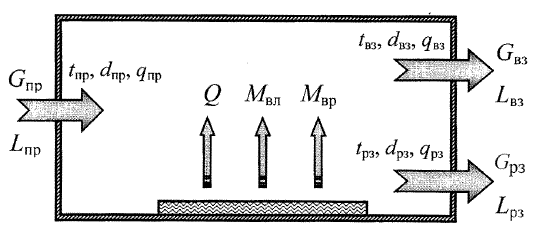
\includegraphics[width=0.5\textwidth]{inc/png/ventilation.png}
  \caption{Схема воздухообмена в помещении}
  \label{fig:ventilation}
\end{figure}

Балансы явной теплоты и воздуха в помещении описываются следующей системой уравнений:
\begin{equation}
	3.6Q + G_{\textup{пр}}c_{p}t_{\textup{пр}} - G_{\textup{вз}}c_{p}t_{\textup{вз}} - G_{\textup{рз}}c_{p}t_{\textup{рз}} = 0;
\label{equ:heat_balance}
\end{equation}
\begin{equation}
	G_{\textup{пр}} - G_{\textup{вз}} - G_{\textup{рз}} = 0,
\label{equ:air_balance}
\end{equation}

где $Q$ -- избытки явной теплоты в помещении, Вт; $c_{p}$ -- удельная теплоемкость воздуха;
$c_{p} \approx 1.0~\textup{кДж}/(\textup{кг} \cdot \celsius)$;
$t_{\textup{пр}},t_{\textup{вз}},t_{\textup{рз}}$ -- температуры соответственно приточного воздуха,
воздуха в верхней и рабочей зонах помещения, \celsius. Обратимся к первому слагаемому в уравнении~\ref{equ:heat_balance},
введя для него обозначение $Q' = 3.6Q$. Так же, как и все остальные слагаемые в этом уравнении, оно имеет размерность~кДж/ч.
Отсюда получим следующее выражение для массового расхода воздуха, удаляемого из верхней зоны:
\begin{equation}
	G_{\textup{вз}} = \frac{Q' - G_{\textup{рз}}c_{p}(t_{\textup{рз}} - t_{\textup{пр}})}{c_{p}(t_{\textup{вз}} - t_{\textup{пр}})}.
\label{equ:top_area_mass_consumption}
\end{equation}

Перейдем в формулах (\ref{equ:air_balance}), (\ref{equ:top_area_mass_consumption}) от массовых расходов к объемным с помощью соотношений
$L_{\textup{пр}} = G_{\textup{пр}} / \rho_{\textup{пр}},
 L_{\textup{вз}} = G_{\textup{вз}} / \rho_{\textup{вз}},
 L_{\textup{рз}} = G_{\textup{рз}} / \rho_{\textup{рз}}$, где $\rho_{\textup{пр}}, \rho_{\textup{вз}}, \rho_{\textup{рз}}$
-- плотности соответственно приточного воздуха и воздуха в верхней и рабочей зонах помещения, $\textup{кг}/\textup{м}^{3}$. В результате получим
\begin{equation}
	L_{\textup{вз}} = \frac{Q' - L_{\textup{рз}}\rho_{\textup{рз}}c_{p}(t_{\textup{рз}} - t_{\textup{пр}})}{\rho_{\textup{вз}}c_{p}(t_{\textup{вз}} - t_{\textup{пр}})}.
\label{equ:top_area_volume_consumption}
\end{equation}
\begin{equation}
	L_{\textup{пр}} = L_{\textup{вз}}\rho_{\textup{вз}}/\rho_{\textup{пр}} + L_{\textup{рз}}\rho_{\textup{рз}}/\rho_{\textup{пр}}.
\label{equ:air_volume_balance}
\end{equation}

Температуру наружного воздуха,~\celsius, для теплого периода года
определяют параметрами А, а для холодного периода года -- параметрами Б (таблица~\ref{tab:temperature_params}).

\begin{table}[ht!]
  \centering
  \caption{Расчетные значения параметров наружного воздуха для Москвы по СП~131.13330-2012}
  \label{tab:temperature_params}
  \begin{tabular}{|c|c|c|}
    \hline
    Период года & Параметры & Температура воздуха, \celsius  \\
    \hline
    Теплый & A & 22.3 \\
    \hline
    Холодный & Б & -26 \\
    \hline
  \end{tabular}
\end{table}

Температура воздуха $t_{\textup{вз}}$, удаляемого из верхней зоны помещения,
зависит от многих факторов, в частности от особенностей организации воздухообмена в помещении. В некоторых
случаях для помещения высотой более 4~м она может быть расчитана по формуле
\begin{equation}
	t_{\textup{вз}} = t_{\textup{рз}} + \Delta(H - 2),
\label{equ:temp_top_zone}
\end{equation}

где $\Delta$ -- градиент температуры по высоте помещения, \celsius/м, зависящий от особенностей теплообмена
в помещении и определяемый, как правило, по результатам натурных измерений; $H$ -- расстояние от пола до
центра вытяжных отверстий в помещении, м. При этом для помещений с незначительными избытками теплоты,
не превышающими $23~\textup{Вт}/\textup{м}^{3}$, полагают $\Delta = 0.2...0.5~\celsius/\textup{м}$; при
значительных избытках теплоты в помещении, превышающих $23~\textup{Вт}/\textup{м}^{3}$, полагают
$\Delta = 0.7...1.5~\celsius/\textup{м}$. Следует отметить, что приведенные значения $\Delta$ применимы только
для схемы воздухообмена <<снизу-вверх>>, т.е. при подаче приточного воздуха в рабочую зону помещения и удалении
нагретого воздуха из верхней зоны. Когда приточный воздух подается в верхнюю зону, значение температурного градиента
будет близко к нулю, так что $t_{\textup{вз}} \approx t_{\textup{рз}}$.

Если значения температуры приточного воздуха и воздуха в помещении отличаются не более чем на 15~\celsius,
то с погрешностью, не превышаюшей 5\%, можно положить $\rho_{\textup{пр}} = \rho_{\textup{вз}} = \rho_{\textup{рз}}$.
При этом уравнения (\ref{equ:top_area_volume_consumption}), (\ref{equ:air_volume_balance}) примут вид
\begin{equation}
	L_{\textup{вз}} = \frac{Q' - L_{\textup{рз}}\rho_{\textup{пр}}c_{p}(t_{\textup{рз}} - t_{\textup{пр}})}{\rho_{\textup{пр}}c_{p}(t_{\textup{вз}} - t_{\textup{пр}})};
\label{equ:top_area_volume_consumption_simple}
\end{equation}
\begin{equation}
	L_{\textup{пр}} = L_{\textup{вз}} + L_{\textup{рз}}.
\label{equ:air_volume_balance_simple}
\end{equation}

Средняя потребляемая мощность ПК составляет 350~Вт, будем считать что $1/3$ переходит в теплоту,
тепловыделения от одного человека составляют 100~Вт таким образом избыток теплоты составляет
$30 \cdot 350/3 + 30 \cdot 100 = 6500$~Вт = 6.5~кВт.

Будем считать, что воздух удаляется только из верхней зоны, т.е. $L_{\textup{рз}} = 0~\textup{м}^{3}/\textup{ч}$.

Для теплого периода года температура наружного воздуха, соответствующая параметрам А (таблица~\ref{tab:temperature_params}),
равна 22.3~\celsius, для холодного -- -26~\celsius (параметры Б).

Определим теперь удельные избытки теплоты в помещении. Для этого вычислим сначала объем помещения
$V = 15 \cdot 9 \cdot 5 = 675~\textup{м}^{3}$. Удельные избытки теплоты $q = 6500 / 675 \approx 10~\textup{Вт}/\textup{м}^3$,
что меньше $23~\textup{Вт}/\textup{м}^3$. Поэтому они являются незначительными.

Положим, что приточный воздух подается в рабочую зону. Тогда температуру в верхней зоне помещений можно определить по
формуле (\ref{equ:temp_top_zone}), приняв $\Delta = 0.5~\celsius/\textup{м}$. Полагая также, что центр вытяжных отверстий располагается на
высоте 4.5~м от пола, находим что температура воздуха в верхней зоне
$t_{\textup{вз.тепл}} = 25 + 0.5(4.5-2) = 26.25~\celsius$ и $t_{\textup{вз.хол}} = 24 + 0.5(4.5-2) = 25.25~\celsius$.

Теперь можно определить расход воздуха в верхней зоне. Согласно (\ref{equ:top_area_volume_consumption_simple}) будем иметь
$L_{\textup{пр.тепл}} = \frac{3.6 \cdot 6500}{1.2 \cdot 1.0 (26.25 - 22.3)} \approx 4937~\textup{м}^{3}/\textup{ч}.$ и
$L_{\textup{пр.хол}} = \frac{3.6 \cdot 6500}{1.2 \cdot 1.0 (25.25 - -26)} = 380.49~\textup{м}^{3}/\textup{ч}.$

Таким образом требуемый воздухообмен составляет $5000~\textup{м}^{3}/\textup{ч}$.

В слишком теплые дни вентиляция будет только ухудшать ситуацию и тогда необходимо использовать кондиционер.

\section{Утилизация пластмасс, являющихся частью жидко-кристаллического монитора}
Процесс переработки начинается с ручного демонтажа составных частей электронной техники.
Демонтированные компоненты, как правило, сортируются на пластик, металл, печатные платы,
провода, люминесцентные лампы, ЖК-дисплеи для дальнейшей переработки.
В данной главе будет рассмотрен процесс утилизации пластика.

Пластмассы — это материалы на основе природных или синтетических полимеров, способные
под воздействием нагревания или давления деформироваться в изделия сложной конфигурации
и затем устойчиво сохранять полученную ими форму. В зависимости от технологического
процесса производства, применяемого наполнителя и связующего (смолы) пластмассы могут
быть композиционными, слоистыми или литыми, а по природе применяемой
смолы — термореактивными или термопластичными.

При производстве пластмасс образуются отходы, которые не могут быть
использованы. Они вместе с бытовыми отходами отправляются на полигон твердых
бытвых отходов (ТБО). Пластмассы мало используются как вторичное сырье из-за многообразия их типов
и сложности их составов. Производство пластмасс не связано с загрязнением сточных
вод, так как по технологии должно быть обеспечено оборотное водоснабжение.

Основные направления утилизации и ликвидации отходов пластмасс таковы:
\begin{enumerate}
\item переработка их по заводской технологии;
\item сжигание совместно с ТБО и промышленными отходами;
\item пиролиз или раздельное сжигание в специальных печах;
\item использование отходов пластмасс как готового материала в других технологических процессах.
\end{enumerate}

Наиболее оптимальным методом использования отходов пластмасс является их
переработка по заводским технологиям~\cite{utilization}. Общая схема процесса переработки
включает следующие стадии:
\begin{enumerate}[1.]
\item отделение непластмассовых компонентов (ветошь, картон, остатки упаковки:
	бумажные, деревянные или металлические) и сортировка отходов по внешнему виду
\item измельчение отходов пластмассы (иногда в несколько стадий) до размеров,
	достаточных для осуществления их дальнейшей переработки
\item отмывка измельченных отходов от загрязнений органического и минерального
	характера
\item классификация и сушка отходов
\item смешивание полученных отходов (при необходимости) со стабилизаторами,
	красителями, наполнителями и гранулируют
\item переработка гранулята в изделия
\end{enumerate}

При качественной предварительной рассортировке пластмасс по видам, достижении высокой
степени очистки и выделения отдельных отходов из смесей их переработка практически не
отличается от переработки первичных пластмасс. При этом необходимо учитывать способность
полимеров сохранять или изменять свойства в процессе многократной переработки, что
вообще определяет целесообразность выполнения переработки отходов. Изменение физико-химических
свойств большинства полимеров при многократной переработке связано со снижением молекулярной
массы пластмасс, разветвленностью их структуры. Снижение молекулярной массы пластмасс
приводит к изменению их прочностных показателей.

Особенностью повторной переработки поливинилхлорида (ПВХ) является необходимость
его дополнительной стабилизации. Отходы мягкого ПВХ используются для получения
бытовых изделий, пленочных покрытий и пленок. При этом 20\% отходов измельчают
на смесительных вальцах, смешивают с товарным ПВХ, красителями, смазками и
стабилизатором, а затем пропускают через систему подогревательных и отделочных
вальцов. Из отходов полиэтилена высокого давления производят мешки для мусора,
трубы, хозяйственные ведра, уплотнительные профили и прокладки. Полипропиленовые
отходы перерабатывают в текстильные шпули, детали сантехники, дверные ручки, ящики для растений.

Выполнение утилизации смесей отходов без предварительного разделения их
составляющих делает процесс утилизации более дешевым, но физико-механические
свойства полученных при этом изделий гораздо хуже.

Таким образом процесс утилизации и переработки пластмасс является актуальной темой.


\backmatter %% Здесь заканчивается нумерованная часть документа и начинаются ссылки и
            %% заключение

\Conclusion

В результате работы по созданию ядра операционной системы была реализована его
основная функция как средства разделения аппаратных ресурсов: физической памяти,
процессорного времени и устройства вывода информации. В итоге была создана
многозадачная однопользовательская однопроцессорная система с монолитным ядром.

Недостатками полученной ОС являются отсутствие файловой системы и поддержки
многопроцессорной архитектуры. Тем не менее, созданная система поддерживает
современную архитектуры процессоров AMD64, реализует
полноценную изоляцию процессов, виртуальную память на основе страниц, вытесняющую
многозадачность, потоки уровня ядра и эффективное клонирование процессов на
основе копирования памяти при ее изменении.

Разработанную операционную систему можно улучшить следующим образом: добавить возможность
работы с несколькими процессорами~\cite{mp} и средства синхронизации,
добавить файловую систему и межпроцессное взаимодействие (англ. IPC), добавить
поддержку дополнительного аппаратного обеспечения, например -- сетевой карты.


% % Список литературы при помощи BibTeX
% Юзать так:
%
% pdflatex rpz
% bibtex rpz
% pdflatex rpz

\bibliographystyle{gost780u}
\bibliography{rpz}

%%% Local Variables: 
%%% mode: latex
%%% TeX-master: "rpz"
%%% End: 


\appendix   % Тут идут приложения

%\chapter{Картинки}
\label{cha:appendix1}



%\chapter{Еще картинки}
\label{cha:appendix2}




\end{document}
